\documentclass{ddis-thesis}
\usepackage{amsmath, amsthm, amssymb}
\usepackage[utf8]{inputenc}
\usepackage{program}
\usepackage{mathrsfs}
\usepackage{amsfonts}
\usepackage{gensymb}
\usepackage{multirow}
\usepackage[capitalise]{cleveref}
\usepackage{subfig}
\usepackage{tabularx}
\usepackage{pdflscape}
\usepackage{scrhack}
\usepackage{breakcites}
\usepackage{natbib}
\usepackage{microtype}
\usepackage[left=2.5cm, right=2.5cm, bottom=2cm, includefoot]{geometry}
\usepackage[margin=15pt,font=small,labelfont={bf,sf}]{caption}
\usepackage{graphicx}

% fonts
\usepackage[scaled=0.95]{helvet}
\usepackage{mathpazo}
\usepackage[euler-digits,euler-hat-accent]{eulervm}

\usepackage{xcolor}
\definecolor{VeryLightGrey}{RGB}{255,253,255}

\usepackage{fancyvrb}
\DefineVerbatimEnvironment{code}{Verbatim}{fontsize=\small}
\DefineVerbatimEnvironment{example}{Verbatim}{fontsize=\small}

\usepackage{fancyhdr}% fancyhdr related command; details in its documentation
\pagestyle{fancy}
\fancyhead{}
\fancyhead[LE,RO]{\thepage}
\fancyhead[RE]{\leftmark}
\fancyhead[LO]{\rightmark}

\usepackage{minted}
\setminted{fontsize=\footnotesize,baselinestretch=0.9,bgcolor=VeryLightGrey}

\author{Roland Schläfli}
\title{Analysis of Weather Data using Graph-based and Neural Network Methods}
\begin{document}

% *************** Front matter ***************
\frontmatter
\begin{titlepage}

\setlength{\textwidth}{16cm}
\setlength{\oddsidemargin}{0cm}
\setlength{\evensidemargin}{0cm}
\setlength{\topmargin}{8mm}
\setlength{\headheight}{0cm}
\setlength{\headsep}{0cm}
\setlength{\topskip}{0cm}
\enlargethispage{5cm}

\noindent
\setlength{\unitlength}{1mm}

\begin{picture}(160,226)
\centering

\put(0,203){\line(1,0){160}} % lower line
\put(109,39){\line(1,0){50}}
\put(109,161){\line(1,0){50}}
\put(109,170){\line(1,0){50}}
\put(107,1){\line(0,1){200}}

\put(0,140){\parbox[b][6em]{100mm}{
    \begin{center}
    \textbf{\Huge{\sffamily{Analysis of Weather Data using Graph-based and Neural Network Methods}}}
    \end{center}}}

\put(109,92){\parbox[b]{50mm}{
    \textbf{{\sffamily{{\Large Roland Schl\"afli}}}}\\
    {\sffamily{of Bern BE, Switzerland\\\\
    Student-ID: 12-932-398\\
    rolandschlaefli@gmail.com
    }}
}}

\put(109,161){\makebox(50,9){{\sffamily{BSc Thesis \hfill January 31, 2018}}}}

\put(0,215){\makebox(80,11)[l]{
\includegraphics[height=2.8cm]
{./00_title/figures/uzh_logo_e_pos}}}


\put(109,32){\parbox[b]{50mm}{\flushleft
    {\sffamily{Advisor:}} {\textbf{\sffamily{Bibek Paudel}} }
    }
}

\put(109,10){\parbox[b]{50mm}{\flushleft
        {\sffamily{
        Prof. Abraham Bernstein, PhD\\
        Institut f\"ur Informatik\\
        Universit\"at Z\"urich\\
        http://www.ifi.uzh.ch/ddis}
        }
}}

\end{picture}
\end{titlepage}



\begin{acknowledgements}
First and foremost, I would like to thank Prof. Bernstein for the opportunity to work on such an interesting problem at his research group.

I am also very grateful for the tremendous support provided by my advisor Bibek Paudel, who was always ready to provide constructive feedback and new ideas. His support made the overall creation of this work a thoroughly enjoyable and interesting process.

I would further like to thank Veronika Stolbova for her willingness to consult with us on our early approaches and results, which has helped us identify some early flaws in our implementation. My thanks also go out to Anja Zgraggen and Pascal Zehnder, who have helped improve the formal and content-related correctness of this work.
\end{acknowledgements}

\begin{zusammenfassung}
Der Indische Sommermonsun ist von grosser Bedeutung für über eine Milliarde Menschen. Die Wichtigkeit einer präzisen statistischen Auswertung des Monsunverhaltens wird dadurch deutlich. In dieser Arbeit analysieren wir die geographische Verteilung von extremem Monsunregenfall und entwickeln eine neue Methode zur Vorhersage des Monsunbeginns. Wir berechnen Netzwerke aus korrelierten Orten auf dem Indischen Subkontinent und analysieren diese mit verbreiteten Indikatoren der Netzwerkzentralität. Dadurch zeigt sich eine relative Wichtigkeit von Regionen wie dem Indischen Ozean, dem Tibetischen Plateau und Nordpakistan. Basierend auf aktuellen Methoden im Bereich der Neuronalen Netzwerke entwickeln wir ausserdem ein neues Modell zur Vorhersage des Monsunbeginns basierend auf räumlich-zeitlichen Wetterdaten. Mit darauf aufbauenden Experimenten zeigen wir, dass unser Modell den Monsunanfang mehrere Tage im Voraus genauer als bestehende Methoden vorhersagen kann.
\end{zusammenfassung}

\begin{abstract}
Each year, the Indian Summer Monsoon affects more than one billion people, making clear the importance of accurate statistical analysis of its behavior. In this work, we analyze the spatial distribution of extreme monsoon rainfall and propose a new way of predicting monsoon onset dates. We build networks of correlated locations on the Indian subcontinent, analyzing them with established centrality measures. These centrality measures reveal the relative importance of locations like the Indian Ocean, the Tibetan Plateau, and Northern Pakistan. We additionally adopt recent advances in machine learning and neural networks to predict monsoon onset dates based on spatiotemporal meteorological datasets. With experiments on these datasets, we show that our model is able to predict onset dates more accurately than existing methods several days in advance.
\end{abstract}


\tableofcontents

% *************** Main matter ***************
\mainmatter

% extend vertical spacing of tabular environments
\renewcommand{\arraystretch}{1.3}

\chapter{Introduction}
\label{c:introduction}

The Indian Summer Monsoon (further also referred to as ISM) is one of the most significant meteorological events on our planet. It shapes the lives of the more than one billion people living in and around India. Many parts of India receive up to 80\% of rainfall during the monsoon season, and significant parts of the population obtain their drinking water from monsoon rainfalls \citep{Stolbova.2015}. Farmers further depend on the arrival of these rainfalls to be able to water their crops and feed their livestock. The monsoon is of similarly high impact for the Indian economy at large, as the country is still dependent on its agricultural sector, which makes up almost one-fifth of India's GDP \citep{CentralIntelligenceAgency.05.01.2018}.

In itself, the ISM is a highly complex climatological phenomenon. It displays considerable variability in both timing and strength and is influenced by many factors on regional and global scales. Due to its obvious importance, the behavior of the ISM has been a focus of climate researchers for many decades, bringing to light many theories and hypotheses. However, even today, some of its characteristics and global teleconnections remain unexplained.

[TODO: extend "motivation"]

Because of the complex behavior of the ISM, we dedicate \cref{c:ism_overview} of this work to a short summarization of research about the inner workings of the ISM. We explain the major factors that are known to influence monsoon as well as theories for those that are still unknown. We also try to further motivate the significance and social impact of the monsoon for the people in India and its surrounding countries.

\begin{figure}[h]
  \centering
  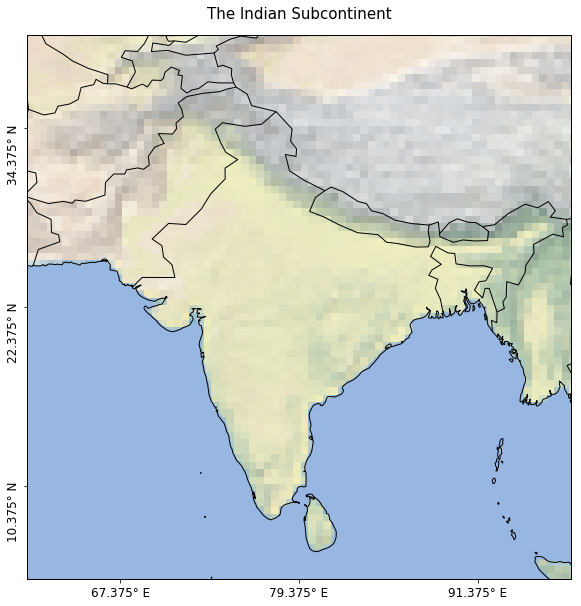
\includegraphics[width=0.5\linewidth]{./99_appendix/img/area_overview}
  \caption{The Indian subcontinent as extracted from TRMM.}
  \label{fig:trmm_area}
\end{figure}

The remainder of this work is then structured into two major parts that are both firmly connected to the behavior of the ISM. The first part (\cref{c:event_sync}) is dedicated to the analysis of extreme precipitation\footnote{Rainfall} events before, during and after the monsoon season. Such events are regularly seen all over India and represent one of the most significant challenges the local population faces from the ISM. Extreme rainfall can cause enormous damage by flooding cities or destruction of essential infrastructure. As such, there is a clear need to analyze and predict the spatial and temporal distribution of these extreme rainfall events.

Strongly basing our first part on the work of \citet{Stolbova.2015}, we extract extreme rainfall events from the TRMM precipitation dataset.

[TODO: short TRMM summary]

We then calculate the synchronicity of different pairs of locations\footnote{Simplified example: two locations are synchronous if an extreme event in one location tends to be followed by an extreme event in the other location.} and build a graph (a ``climate network'') connecting the most significantly synchronous locations.

Analysis of the resulting graph using graph centrality measures\footnote{Degree, Betweenness and PageRank} finally shows us the locations that are the most central and important in the graph. This knowledge could potentially help in the analysis or even prediction of monsoon behavior. For example, extreme rainfall in a location that is very central might be a reason to implement additional safety measures in connected locations.

The second major part of this work (\cref{c:part2}) deals with another critical issue regarding the Indian Summer Monsoon: the prediction of the onset date of monsoon. The onset date for a location in India depicts the point at which the monsoon reaches said location with strength and durability above a predefined threshold. We try to predict such an onset date for the Kerala region, which is generally one of the first locations reached by the ISM and as such marks the beginning of monsoon for the whole Indian subcontinent.

[TODO: short ERA-Interim summary]

For our onset prediction task, we build several neural network architectures using the Python Keras 2.0 and Tensorflow 1.4 libraries and describe the intuition of each. Experiments with each model allow us to evaluate and shortly summarize our most important findings. We iteratively improve upon the findings of each model, building models with vastly different architectures as well as for a number of datasets, features and combinations thereof (TRMM, ERA-Interim, different sets of onset dates). An overview and comparison of the learning capabilities of all models then serves as a conclusion to the second part.

Finally concluding our work in \cref{c:conclusion}, we summarize our overall findings and try to interpret the results of \cref{c:event_sync} and \cref{c:part2}. We additionally provide ideas for the improvement of our work and possible future research based on the topics of extreme event synchronization and monsoon onset prediction using neural networks.

\chapter{An Overview of the Indian Summer Monsoon}
\label{c:ism_overview}
The Indian Summer Monsoon is a global climatic phenomenon that has been actively researched for decades. Even though many theories and hypotheses exist, the factors influencing its strength, timing and variability have still not been fully identified and understood. This chapter aims to provide a short overview of the observed behavior and current scientific understanding of ISM, as far as the foreknowledge might prove useful for the further parts of this work.

\section{Seasons \& Progression}
\label{st:ism_seasons}
The ISM progresses over the Indian subcontinent in three main phases: the pre-monsoon season (March-May), the primary monsoon season (June-September) and the post-monsoon season (October-December) \citep{Stolbova.2015}.

The months of the pre-monsoon season correspond to the Indian summer and are characterized by high temperatures with low amounts of rainfall over regions in the Himalayas and south-west India. Many predictions about the further development of ISM are commonly based on the pre-monsoon season, especially on the patterns that occur leading up to the primary monsoon season \citep{Stolbova.2015}.

A sudden transition with rapidly increasing amounts of daily rainfall, moisture, and kinetic energy, as well as increased vertical shear in horizontal winds\footnote{A gradient between wind speeds at different heights or pressure levels.}, then marks the beginning of the primary monsoon season \citep{Pradhan.2017}. This transition, the "onset" of monsoon, occurs at different times for different parts of the Indian subcontinent as can be seen in \cref{fig:onset_propagation}. First arriving in Kerala on the southwestern tip of the subcontinent around the first of June, the ISM then propagates north- and northwestwards, where it reaches the Pakistani border around the 15th of July \citep{Willetts.2017}.

\begin{figure}[h]
  \centering
  [TODO: image for onset propagation (use stolbova?)]
  \caption{Propagation of monsoon over the Indian subcontinent.}
  \label{fig:onset_propagation}
\end{figure}

After the ISM has fully covered the Indian subcontinent in July, most places experience strong weather conditions well into ...

[TODO: describe withdrawal of monsoon and its timing]

[TODO: describe post-monsoon phase and the northeast monsoon]

\section{Main Drivers}
\label{st:ism_factors}
In its most basic form, the ISM can be seen as a sea breeze of enormous extent. The hot summer weather during the pre-monsoon season causes a heating of the Indian subcontinent. An increasingly large temperature gradient due to slower heating of the Indian Ocean then causes air to flow onto the subcontinent, bringing with it the moisture necessary to cause precipitation \citep{Willetts.2017}.

Intense heating and heat dissipation of the high-altitude Tibetan Plateau lead to an increase in the tropospheric temperature, creating an area of low-pressure near the surface that attracts moisture from surrounding areas over the Indian Ocean [TODO: cite stolbova and secondary]. The low-pressure zone further causes strong vertical air currents from south of the Tibetan Plateau, aiding the ISM with its propagation into the far north of India \citep{Pradhan.2017} [TODO: cite li\&yanai or so].

On a larger scale, the ISM has been linked to several parts of the global atmospheric circulatory system. A shift of the subtropical jet stream to the north of the Tibetan Plateau [TODO: cite yin?] as well as interaction with the westerly jet stream have been found to influence the behavior of the ISM \citep{Ordonez.2016, Stolbova.2015}. A strong westerly jet in the lower troposphere over Kerala seems to generally correlate with the monsoon onset of the region \citep{Ordonez.2016} [TODO: cite rao?]. Additionally, the Somali jet passing over the Arabian sea cools down the body of water, further strengthening the temperature gradient \citep{Stolbova.2015}.

The trade winds of the northern and southern hemisphere meet to create the Intertropical Convergence Zone (ITCZ), a belt of low-pressure close to the thermal aequator. When the ITCZ moves north following the summer months, it further increases the variability of weather events and thus reduces their predictability \citep{Stolbova.2015}.

A further factor in the development and strength of the ISM is the El Niño Southern Oscillation (ENSO). The warming of the Humboldt ocean current during El Niño years causes the land-ocean temperature gradient to decrease. This tends to decrease the amount of rainfall the Indian subcontinent receives and can delay the onset of monsoon by several days \citep{Pradhan.2017, Willetts.2017}. Conversely, the cooling of the current during La Niña can result in more rainfall and an earlier onset due to a higher temperature gradient.

A combination of the above factors creates a low-pressure channel (a "monsoon through") closely south of and parallel to the Tibetan Plateau that serves as a main source of moisture during the ISM \citep{Stolbova.2015}.

This summarization of the impacting factors of the ISM is not exhaustive, as the ISM is much more complex and some of its behavior has still not been fully explained. However, knowledge of these basic factors should already provide a good intuition for \cref{c:event_sync} and \cref{c:part2}.

\section{Social Impact}
\label{st:ism_impact}
As we have already seen, the Indian Summer Monsoon is one of the most impactful large-scale meteorological events on earth. It affects the lives of up to one-fourth of the world's population: the people living on and around the Indian subcontinent \citep{Stolbova.2015}. The heavy rainfalls that the ISM brings with it are of great importance for the population in India and surrounding countries.

Livelihood on the Indian subcontinent is strongly coupled to a timely occurrence of the ISM. Monsoon rainfalls are responsible for 80 percent of the annual precipitation on the Indian subcontinent \citep{Jin.2017}. Farmers depend on these rainfalls to water their crops and feed their livestock. Up to 2012, more than half of a year's rice harvest was still grown during the monsoon period \citep{Auffhammer.2012}.

The agricultural sector accounts for almost one-fifth of the India's GDP, and about 50\% of the population in India either directly or indirectly depend on the agricultural sector [TODO: cite CIA Factbook]. Monsoon rainfalls further provide the majority of drinking water in many parts of India \citep{Stolbova.2015}.

The impactfulness of ISM makes clear the need of being able to predict the monsoon onset and withdrawal dates accurately. If farmers knew in advance when monsoon rainfalls would start, they could wait until the appropriate time to plant their crops. On the contrary, if they get surprised by either early or late onset of monsoon, their crop yield might be reduced, or their crops destroyed entirely.

[TODO: IMD and its predictions]

[TODO: more?]

\section{Trends \& Outlook}
\label{st:ism_trends}

Much like the global climate, the ISM is exposed to climate change and other trends that can impact its variability and predictabily significantly. A major trend that was prevalent during the second half of the 20th century was a decrease in precipitation over northern-central India (close to the Tibetan Plateau) \citep{Jin.2017}.

[TODO: cite Jin 6,7] propose that such a drying trend could be connected to a warming of the surrounding Indian Ocean. A resulting weakening of the land-ocean temperature gradient could have been responsible for the lower rainfall amounts. A further hypothesis states that large-scale deforestation could have decreased the amount of transpiration from plants, resulting in less moisture and thus precipitation [TODO: cite Jin 8].

[TODO: reversal of drying trend]

[TODO: general climate change]

[TODO: more?]






\chapter{Part 1: Synchronization of Extreme Events}
\label{c:event_sync}
During the primary monsoon season, floodings and landslides caused by extreme rainfall can lead to massive societal and environmental damage \citep{Stolbova.2015}. It is thus crucial to be able to analyze, detect and potentially predict such extreme rainfall events, especially as their proportion tends to further increase with global warming \citep{Stolbova.2015} [TODO: cite Goswami?].

A way of analysis that \citet{Stolbova.2015} has proposed is the computation of climate networks based on different locations in India, followed by an analysis of the resulting networks using centrality measures. We strongly base this chapter on her work and thus summarize her approach in \cref{sst:event_sync}. We also explain the network measures that will be applied to the resulting climate networks (\cref{sst:network_measures}) and introduce the dataset that will be used as a basis for all calculations (TRMM, \cref{sst:trmm_dataset}).

\cref{st:event_sync_implementation} then provides an overview of our approach to the creation of climate networks and explains where our approach differs from the work of \citep{Stolbova.2015}. Following up in \cref{st:event_sync_results}, we analyze and visualize the computed climate networks using centrality measures and try to interpret the results in contrast to the known factors of monsoon behavior. Concluding this chapter in \cref{st:event_sync_conclusion}, we elaborate the usefulness of our results and how they could be improved upon.

\section{Related Work}
[TODO: need text here?]

\subsection{The TRMM dataset}
\label{sst:trmm_dataset}
The Tropical Rainfall Measurement Mission (TRMM) is a precipitation research effort by the National Aeronautics and Space Administration (NASA) and the Japanese Aerospace Exploration Agency (JAXA). It is based on the TRMM observatory, a satellite that was launched into space on the 27th of November, 1997. The products based on TRMM range from the raw output of the multitude of sensors on the satellite to the highly aggregated and gridded rainfall estimates we will be using in this work \citep{GoddardEarthScienceDataInformationandServicesCenter.2016}.

More specifically, the TRMM product that we will be using is a 3-hourly estimate of surface rainfall aggregated from the satellite sensors in combination with surface gauge values and imagery from other satellites. This product is referred to as 3B42 or TMPA and is also available in a daily variation, where the eight 3-hourly measurements (i.e., 00:00, 03:00, 06:00 and so on) have been summed up to provide a single daily rainfall estimate.

[TODO: update coordinates and grid specifics] 3B42 is available for the area between 50\degree N. and 50\degree S. We subset this area to cover the entire Indian subcontinent (x-x\degree N, x-x\degree E). These border coordinates are a superset of the ones used in \citep{Stolbova.2015}: the grid has been extended  such that it can be cleanly aggregated from a 0.25\degree spatial resolution to the 0.75\degree resolution of the ERA-Interim dataset (which we will use later on). \cref{fig:trmm_area} shows the excerpt of the TRMM dataset that we will be using in this work.

\begin{figure}[h]
  \centering
  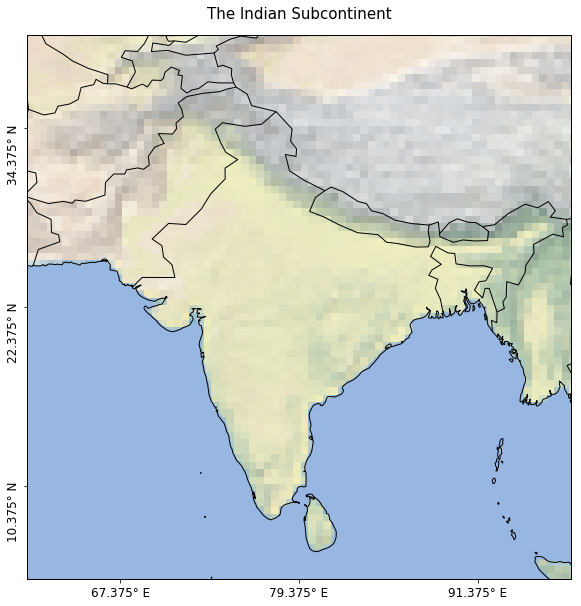
\includegraphics[width=0.5\linewidth]{./99_appendix/img/area_overview}
  \caption{The Indian subcontinent as extracted from TRMM.}
  \label{fig:trmm_area}
\end{figure}

The TRMM dataset is unique in that it offers very high-resolution precipitation estimates since January 1998. It can prove useful for research based on the distribution, frequency, and intensity of rainfall, i.e., for calculating extreme rainfall events \citep{Stolbova.2015}. However, it has to be taken into consideration that the TRMM products are based on complex algorithms and have been derived from different sensors and sources \citep{Huffman.2017b}.

After the TRMM satellite's fuel went low in 2014, it was decommissioned in April 2015 and re-entered earth's atmosphere in June 2015. The TMPA product is still being produced until 2018, albeit without the sensors of the TRMM observatory and with less accuracy \citep{Huffman.2017}.

Built on the success of the TRMM mission, NASA and JAXA have launched its successor GPM (Global Precipitation Measurement) in 2014 \citep{GoddardEarthScienceDataInformationandServicesCenter.2011}. However, as its data is only available starting from 2014, GPM is currently unsuitable for long-term precipitation research. TRMM or an alternative dataset are currently still needed but the updated algorithm developed for GPM will soon be applied to the existing TRMM data. The availability of reprocessed data back to 1998 can thus be expected in 2018 \citep{Huffman.2016}.


\subsection{Event synchronization \& climate networks}
\label{sst:event_sync}
The concept of event synchronization applied in \citet{Stolbova.2015} as well as in our work was first defined in \citet{QuianQuiroga.2002}. \citet{QuianQuiroga.2002} sought to develop a simple algorithm that could be applied to any two time series of events, resulting in a measure that defines the synchronization of said time series. Synchronization measures are generally related to standard measures like cross correlation. They can, however, convey more complex relationships due to their non-linearity \citep{QuianQuiroga.2002}.

\subsubsection{Basic event synchronization}
The basic principle of the event synchronization measure as found in \citet{QuianQuiroga.2002}, \citet{Malik.2010} and \citet{Stolbova.2015} is setup as follows: given the two time series $i$ and $j$ and their respective events $l$ and $m$ occuring at times $t^i_l$ and $t_j^y$, we measure the synchronicity for all possible pairs of events between both series. We classify events as synchronous if they occur closely simultaneous, i.e., within a certain range from each other. This allowed range of occurrence is called \textit{time lag} and is calculated by taking the minimum interevent distance $\tau^{ij}_{lm}$ like so\footnote{If event rates were fixed, a global time lag $\tau$ could be defined, greatly simplifying calculations.}:

\begin{equation}
\tau^{ij}_{lm} = 0.5 * min\left\{t^i_{l+1} - t^i_l, t^i_l - t^i_{l-1}, t^j_{m+1} - t^j_{m}, t^j_{m} - t^j_{m-1}\right\}
\end{equation}

The synchronicity $J$ of any two events $t_i^x$ and $t_j^y$ is then calculated as follows:

\begin{equation}
  J_{ij} =
  \begin{cases}
    1, & \text{if } 0<t^x_i-t^y_j\leq\tau_{ij}, \\
    0.5, & \text{if } t^x_i=t^y_j, \\
    0, & \text{else.}
  \end{cases}
\end{equation}

Applying this to the full time series $i$ and $j$, the number of synchronous events where an event in $i$ leads an event in $j$ is defined like:

\begin{equation}
  c(i \mid j) = \sum\limits^{s_i}_{l=1} \sum\limits^{s_j}_{m=1} J_{ij}
\end{equation}

The same formula applies to the reversed situation, i.e. $c(j \mid i)$, with $s_i$ and $s_j$ being the number of events in the respective time series. Combining the results of $c(i\mid j)$ and $c(j \mid i)$ and normalizing them by the total numbers of events $s_i$ and $s_j$, the \textit{strength of synchronization} is defined as

\begin{equation} \label{eq:sync_strength}
  Q_{ij} = \frac{c(i \mid j) + c(j \mid i)}{\sqrt{(s_i - 2)(s_j - 2)}}
\end{equation}

where $Q_{ij} = 1$ means that the time series are completely synchronized, i.e., that each event in $i$ is either synchronously lead or followed by an event in $j$.

\subsubsection{Application to climate networks}
\label{ssst:appl_climate_networks}
While the work of \citet{QuianQuiroga.2002} focuses on the analysis of EEG\footnote{EEG: Electroencephalogram; A way of measuring brain activity.]} time series, their event synchronization approach is explicitly applicable to other domains. The works of \citet{Malik.2010} and \citet{Stolbova.2015} both expand upon simple event synchronization. For the purposes of our work, we focus on the approach using climate networks as found in \citet{Stolbova.2015}.

Looking at the TRMM dataset as shown in \cref{fig:trmm_area}, each cell of its coordinate grid represents a separate precipitation time series. As the analysis of each monsoon season is performed seperately, one such coordinate grid per season needs to be extracted\footnote{The time series are then simply the respective months of each year, concatenated into a single series.}.

The time series in the resulting grids are not event based and thus cannot be directly used to calculate synchronization. They can, however, easily be transformed into event series by extracting only the days where extreme rainfall occurred. As per \citet{Stolbova.2015}, such days are generally defined as days with rainfall that exceeds the 90th percentile for the respective location.

The resulting series of extreme events can be used to calculate the synchronicity of different locations (grid cells) in the TRMM dataset. Computing the synchronicity for all possible permutations of two such locations then results in a synchronization matrix as can be seen in \cref{fig:synchronization_matrix}.

\begin{figure}[h]
  \centering
  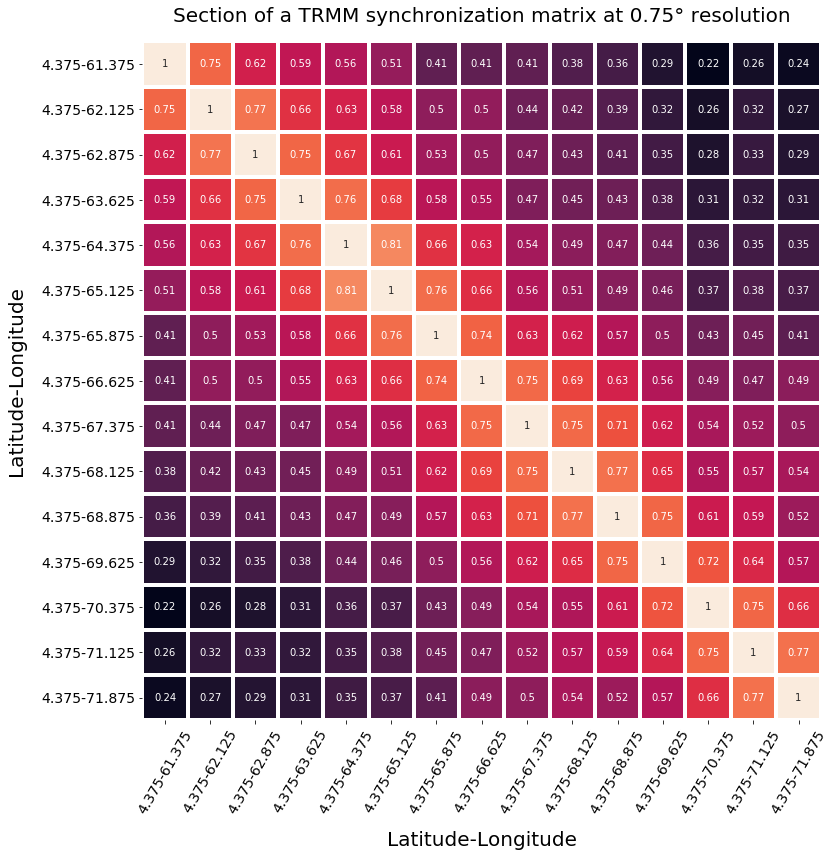
\includegraphics[width=0.65\textwidth]{./99_appendix/img/trmm_sync_example}
  \caption{Exemplary synchronization matrix for TRMM at a 0.75\degree resolution. We only show the top left 15x15 section of our actual matrix, as its full dimensions are 2401x2401 for a 0.75\degree resolution.}
  \label{fig:synchronization_matrix}
\end{figure}

Applying a numerical threshold to this synchronization matrix results in a matrix that contains only the most significantly synchronous values. Everything else is set to zero, including the diagonal of the matrix, as this would result in loops in the graph later on. Additionally, all elements above the threshold are set to one, yielding the adjacency matrix for an undirected, unweighted network (\cref{fig:adjacency_matrix}). \citet{Stolbova.2015} uses the 95th percentile for the threshold applied, as this removes all but the most statistically significant values.

\begin{figure}[h]
  \centering
  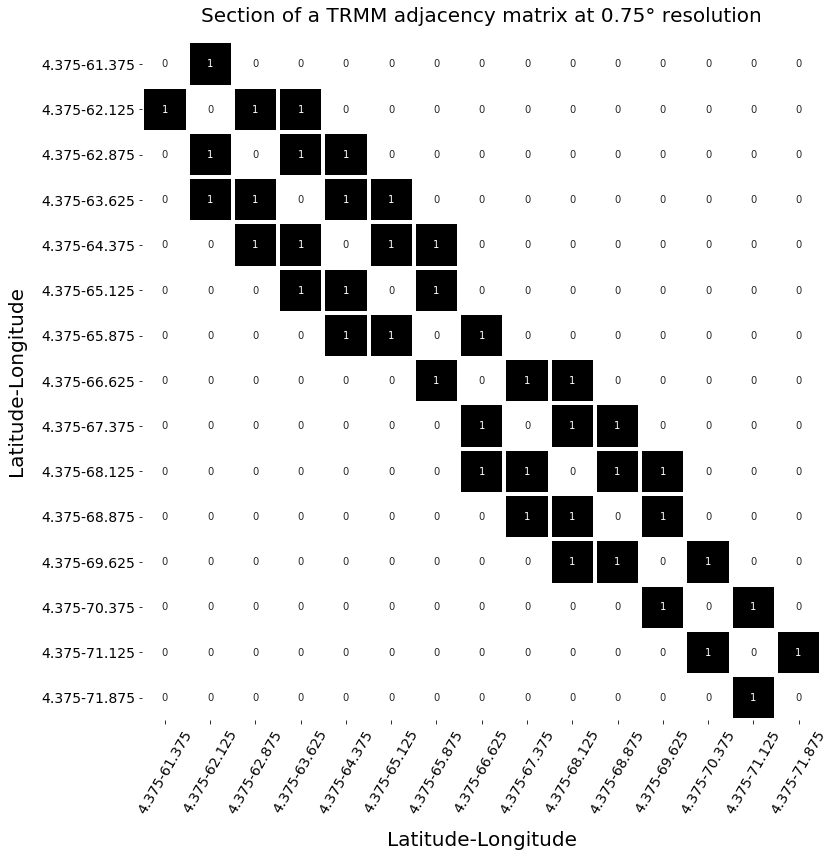
\includegraphics[width=0.65\textwidth]{./99_appendix/img/trmm_adjacency_example}
  \caption{Exemplary adjacency matrix for TRMM at a 0.75\degree resolution. We only show the top left 15x15 section of our actual matrix, as its full dimensions are 2401x2401 for a 0.75\degree resolution.}
  \label{fig:adjacency_matrix}
\end{figure}

Based upon the adjacency matrix, a network can then be computed and analyzed. However, before we detail our implementation of it, the next section briefly describes the measures that we will be using for said network analysis.

\subsection{Graph centrality}
\label{sst:network_measures}
Constructing climate networks from an adjacency matrix as seen in \cref{ssst:appl_climate_networks} enables the analysis of their structural features using various graph-based measures. We now shortly go over the concepts of the measures that we apply to our networks in this work.

The climate networks in \citet{Stolbova.2015} are analyzed using the \textit{degree} and \textit{betweenness} of nodes as well as using the \textit{average/maximal geographical link length} between them. We also base our analysis on the \textit{degree} and \textit{betweenness} measures but replace the link length calculations with the PageRank algorithm, which could, in our opinion, show more distinct patterns than the other two measures.

The \textit{degree} of a node in a network is quite simply defined as the amount of links that are connected to the respective node. The same holds for vertices in graphs and their connected edges.

Calculating the \textit{betweenness} or \textit{betweenness centrality} of a node is a more involved effort. A node has a high betweenness if a large portion of shortest paths in the network pass through the respective node. If the resulting betweenness is to be an exact measure, this basically necessitates the calculation of all shortest paths in the network, which gets increasingly complex with the size of the network. There are, however, algorithms that achieve both accuracy and speed when calculating betweenness, one of the most popular being the approach proposed by \citet{Brandes.2001}\footnote{This algorithm is also used by the Python library \textit{networkx}, which we will be using for our calculations.}.

The final measure that we will apply to climate networks, the \textit{PageRank} algorithm, was originally developed and published by the founders of Google (amongst others), Larry Page and Sergey Brin, during their studies at Stanford University \citep{Page.1999}.

[TODO: finish page rank]

\section{Implementation}
\label{st:event_sync_implementation}
Our implementation of the event synchronization and climate network computations is strongly based on the concepts and measures as described in \cref{sst:event_sync} and \cref{sst:building_climate_network}. As our algorithmic implementation is most certainly different than the one used in the original work \citep{Stolbova.2015}, we shortly go over our approach to the problem in this section.

\subsection{Calculating event synchronization}
\label{sst:event_sync_calculation}

\subsubsection{Necessary preparations}
Before we are able to calculate the synchronicity for any two locations, the precipitation time series need to be transformed into series of events. Assume that we have extracted pre-monsoon time series as shown in \cref{tab:example_rainfall_ts} from the TRMM dataset and now want to convert these into extreme event series.

\begin{table}[h]
  \centering
  \begin{tabular}{ |c|c|ccccccc| }
    \hline
    Latitude & Longitude & 01.03.98 & ... & 29.05.98 & 30.05.98 & 31.05.98 & 01.03.99 & ...\\
    \hline
    13.375 & 67.375 & 0.0  & ... & 0.12 & 2.31  & 2.85  & 0.00 & ... \\
    16.375 & 91.375 & 0.0  & ... & 0.09 & 34.80 & 49.49 & 0.00 & ... \\
    34.375 & 67.375 & 0.52 & ... & 0.00 & 0.00  & 0.00  & 0.00 & ... \\
    34.375 & 88.375 & 0.86 & ... & 2.01 & 51.85 & 68.72 & 0.29 & ... \\
    \hline
  \end{tabular}
  \caption{Precipitation time series during pre-monsoon at 4 exemplary locations (TRMM, 0.75\degree).}
  \label{tab:example_rainfall_ts}
\end{table}

We calculate the 90th percentile seperately for each row and apply the result as a threshold to the respective row. This yields event series where each value represents the date of an extreme event in the series. This would look as shown in \cref{tab:example_rainfall_events} if applied to the time series in \cref{tab:example_rainfall_ts}.

\begin{table}[h]
  \centering
  \begin{tabular}{ |c|c|ccccccc| }
    \hline
    Latitude & Longitude & 1 & 2 & 3 & 4 & 5 & 6 & ... \\
    \hline
    13.375 & 67.375 & 07.04.98 & 31.05.98 & 08.05.99 & 12.05.99 & 13.05.99 & 15.05.99 & ... \\
    16.375 & 91.375 & 17.05.98 & 18.05.98 & 19.05.98 & 30.04.99 & 01.05.99 & 05.05.99 & ... \\
    34.375 & 67.375 & 03.03.98 & 29.03.98 & 02.04.98 & 03.04.98 & 09.04.98 & 22.04.98 & ... \\
    34.375 & 88.375 & 18.03.98 & 30.03.98 & 31.03.98 & 01.04.98 & 05.04.98 & 19.04.98 & ... \\
    \hline
  \end{tabular}
  \caption{First events in the pre-monsoon extreme event series at 4 exemplary locations (TRMM, 0.75\degree).}
  \label{tab:example_rainfall_events}
\end{table}

With a matrix of extreme events as shown in excerpt in \cref{tab:example_rainfall_events}, we then want to calculate the event synchronization for all pairs of locations. \cref{tab:example_empty_sync} shows the state of a preliminary synchronization matrix before running any of the calculations. Locations are always perfectly synchronous to themselves, leading to a diagonal that will always be filled with ones.

\begin{table}[h]
  \centering
  \begin{tabular}{ |cc|cccc| }
    \hline
     & Latitude & 13.375 & 16.375 & 34.375 & 34.375 \\
    Latitude & Longitude & 67.375 & 91.375 & 67.375 & 88.375 \\
    \hline
    13.375 & 67.375 & 1 &   &   &   \\
    16.375 & 91.375 &   & 1 &   &   \\
    34.375 & 67.375 &   &   & 1 &   \\
    34.375 & 88.375 &   &   &   & 1 \\
    \hline
  \end{tabular}
  \caption{Empty synchronization matrix for 4 exemplary locations (TRMM, 0.75\degree).}
  \label{tab:example_empty_sync}
\end{table}

To further fill in the values of the synchronization matrix in \cref{tab:example_empty_sync}, our algorithm only needs to perform calculations for one of the now empty halves of the matrix. This is due to the fact that, at least in our approach, the synchronization between two locations can be symmetrically applied to both their permutations. The original work on event synchronization by \citet{QuianQuiroga.2002} describes some asymmetrical measures, that were, however, not used in the work of \citet{Stolbova.2015}.

Going forward, we use \textit{unix timestamps}\footnote{Unix timestamps measure the number of seconds (without leap seconds) that have elapsed since the 01.01.1970 at 00:00 UTC. For example, "01.03.1998 00:00" would be represented as 888710400.} to represent dates instead of the full representation shown in the examples of this section, as they are much easier to process using mathematical formulas (but less intuitive to visualize).

\pagebreak
\subsubsection{Synchronization of two locations}
Having explained the necessary setup of the event synchronization algorithm, we now go over some of the concepts of our implementation. To calculate the synchronization between any two locations (i.e., \textit{location1} and \textit{location2}), we need to process both time series and compare each event in \textit{location1} to the appropriate events in \textit{location2}, taking the immediate neighbors of both locations into account.

We found that this naturally fits the description of a sliding window approach: a sliding window of size three over the event series of a location always encompasses a current event, its predecessor and its successor and thus everything we need for the time lag calculation. Application of a sliding window to \textit{location1} and nesting another such window for \textit{location2} then leads us to a naive implementation of the event synchronization algorithm as shown in \cref{lst:event_synchronization}.

\begin{listing}[H]
  \begin{minted}[mathescape,
    linenos,
    numbersep=5pt,
    gobble=4,
    frame=lines,
    framesep=2mm]{python}

    def calculate_synchronization(location1, location2):
        # initialize the number of synchronous events for the two locations
        num_sync_events = 0

        # iterate over all timesteps in location1 using a sliding window
        for i_prev, i_current, i_next in sliding_window(location1, 3):

            # iterate over all timesteps in location2 using a sliding window
            for j_prev, j_current, j_next in sliding_window(location2, 3):

                # calculate the time delta between the current events
                current_diff = i_current - j_current

                # check if the current events occur simultaneously
                if current_diff == 0:
                    num_sync_events += 0.5
                    continue

                # calculate the time lag based on the two sliding windows
                time_lag = 0.5 * min(
                    i_next - i_current, i_current - i_prev,
                    j_next - j_current, j_current - j_prev)

                # decide whether the events are synchronous
                if 0 < current_diff <= time_lag:
                    num_sync_events += 1.0

        return num_sync_events

  \end{minted}
  \caption{Python pseudocode for a simplified event synchronization algorithm, applicable to any two series of events.}
  \label{lst:event_synchronization}
\end{listing}

The event synchronization algorithm as described in \cref{lst:event_synchronization} results in the number of synchronous events between \textit{location1} and \textit{location2} where the event in \textit{location2} leads the event in \textit{location1}. This is, however, only part of the full synchronization synchronization calculation, as we also need the number of synchronous events where \textit{location1} leads \textit{location2}, i.e., we need to evaluate $calculate\_synchronization(location2, location1)$. This is the reason that simultaneous events only count as "half synchronous": they are counted in both these calculations and, in total, then result in one synchronous event.

Calculating the strength of synchronization then boils down to a simple application of formula \eqref{eq:sync_strength} from \pageref{eq:sync_strength} and is further presented in \cref{lst:sync_strength}.

\begin{listing}[H]
  \begin{minted}[mathescape,
    linenos,
    numbersep=5pt,
    gobble=4,
    frame=lines,
    framesep=2mm]{python}

    def calculate_sync_strength(loc1_events, loc2_events):
        # calculate synchronized events between loc1 and loc2 (and reverse)
        loc1_sync = calculate_synchronization(loc1_events, loc2_events)
        loc2_sync = calculate_synchronization(loc2_events, loc1_events)

        # calculate the strength of synchronization
        sync_strength = (loc1_sync + loc2_sync) / \
            math.sqrt((len(loc1_events) - 2) * (len(loc2_events) - 2))

        # return the strength of synchronization
        # and the total and separate numbers of synchronous events
        return sync_strength, loc1_sync + loc2_sync, loc1_sync, loc2_sync

  \end{minted}
  \caption{Python pseudocode for the calculation of the synchronization strength between any two series of events.}
  \label{lst:sync_strength}
\end{listing}

\subsubsection{Computing the values of the synchronization matrix}
We then make use of \cref{lst:sync_strength} to fill in the missing values in a synchronization matrix like the one we have already prepared (see \cref{tab:example_empty_sync}). Firstly, the algorithm is applied to each empty cell in the upper half of the matrix, yielding a triangular matrix. Secondly, as the synchronization strength measure is symmetrical, the lower half of the matrix is filled by simply mirroring the upper half. This yields two matrices: one containing the synchronization strength and one containing the total count of synchronous events for all pairs of locations. A third asymmetrical matrix seperately contains the number of events where $i$ leads $j$ as well as the number of events where $j$ leads $i$. The procedure is shown in detail in \cref{lst:sync_matrix}.

\begin{listing}[H]
  \begin{minted}[mathescape,
    linenos,
    numbersep=5pt,
    gobble=4,
    frame=lines,
    framesep=2mm]{python}

    def calculate_sync_matrix(event_matrix):
        # calculate the sync strength for each permutation of grid cells
        for i in range(0, sync_matrix.shape[0]):
            # as the matrix is symmetrical, only calculate the upper half
            for j in range(0, i + 1):
                # calculate the synchronicity for the permutation of rows
                sync_strength, count = calculate_sync_strength(
                    event_matrix[i], event_matrix[j])

                # save results in the respective matrices
                sync_matrix[i, j] = sync_strength
                sync_matrix[j, i] = sync_strength
                count_matrix[i, j] = count
                count_matrix[j, i] = count
                directed_matrix[i, j] = i_leads
                directed_matrix[j, i] = j_leads

        return sync_matrix, count_matrix, directed_matrix

  \end{minted}
  \caption{Python pseudocode for processing an entire event matrix.}
  \label{lst:sync_matrix}
\end{listing}

\subsubsection{Improvements for the event synchronization algorithm}
The implementation as shown so far naively processes all possible combinations of events when calculating the event synchronization measure. Given $i$ events at \textit{location1} and $j$ events at \textit{location2}, the simple nested loop algorithm potentially calculates a time lag up to $i * j$ times. This results in a lot of wasted computation, because the actual portion of $j$ that can be synchronous tends to be very small.

\begin{listing}[H]
  \begin{minted}[mathescape,
    linenos,
    numbersep=5pt,
    gobble=4,
    frame=lines,
    framesep=2mm]{python}

    def calculate_synchronization(location1, location2):
        # initialize the number of synchronous events for the two locations
        num_sync_events = 0

        # iterate over all timesteps in location1 using a sliding window
        for i_prev, i_current, i_next in sliding_window(location1, 3):
            # calculate the last timestamp of location2 that could be synchronous
            latest = i_current + 0.5 * min(i_current - i_prev, i_next - i_current)

            # iterate over all timesteps in location2 using a sliding window
            for j_prev, j_current, j_next in sliding_window(location2, 3):
                # continue for timestamps that cannot possibly be synchronous
                if j_current < earliest:
                    continue

                # if the difference gets negative, continue
                # the second pass will encompass these combinations
                if current_diff < 0:
                    continue

                # check if the events occur simultaneously
                if current_diff == 0:
                    num_sync_events += 0.5
                    continue

                # break for timestamps that cannot possibly be synchronous
                # i.e. are much too late
                if j_current > latest:
                    break

                # calculate the time lag based on the two sliding windows
                time_lag = 0.5 * min(
                    i_next - i_current, i_current - i_prev,
                    j_next - j_current, j_current - j_prev)

                # decide whether the events are synchronous
                if 0 < current_diff <= time_lag:
                    num_sync_events += 1.0

        return num_sync_events

  \end{minted}
  \caption{Python pseudocode for an improved version of the event synchronization algorithm, applicable to any two series of events.}
  \label{lst:event_synchronization_improved}
\end{listing}

However, we can define a range of events in $j$ for which we are sure that they cannot be synchronous and skip their evaluation (see an improved version of the algorithm in \cref{lst:event_synchronization_improved}). According to our implementation, this holds for two cases: firstly, if the event in $j$ occurs at earlier than the event in $i$, it can be safely skipped, as the reversed iteration of the algorithm will deal with it. Secondly, an event in $j$ can also be skipped if the event in $j$ occurs later than the time lag of the event in $i$. Additionally, we can safely break the inner loop early, as further events in $j$ only occur even later.

Notice that another (obvious) improvement would be to "simply filter" the \textit{location2} series such that it only contains the few events that need to be evaluated, after which no more breaking or skipping in the loop would be needed. However, upon evaluation of such an approach, it became clear that this is not necessarily faster. Adequately filtering the series $j$ necessitates some complex indexing and selection operations, which in turn depend on the existence of an index or hash table for $j$. Creating such indices can take more than a second for a single series, making the approach especially slow for large matrices.

\subsection{Building climate networks}
\label{sst:building_climate_network}
Based on \cref{ssst:appl_climate_networks}, the next step after the computation of a full event synchronization matrix is the transformation of said matrix into an adjacency matrix, allowing the creation of a network and its analysis using various methods and libraries. This transformation is a simple thresholding of the matrix using a specified percentile.

\citet{Stolbova.2015} uses the 95th percentile to threshold the adjacency matrix, leaving only the most statistically significant links in the network. However, we use an aggregated {0.75\degree} resolution for our base dataset (instead of the full {0.25\degree} resolution), meaning that there is already much less data available to analyze (but the data is also less sparse). We thus use a decreased threshold equal to the 90th percentile.

We further expand upon the work of \citet{Stolbova.2015} by building weighted networks in addition to the unweighted networks that have already been explored. To build a weighted network, values above the threshold are left as is, leading to links that are weighted with their corresponding synchronization measure. Contrarily, all values above the threshold are uniformly set to one when building an unweighted network.

The creation of a climate network based on an adjacency network, as well as the calculation of the degree, betweenness and PageRank for all nodes in the network, are a matter of a few lines of code as shown in \cref{lst:climate_networks}.

\begin{listing}[H]
  \begin{minted}[mathescape,
    linenos,
    numbersep=5pt,
    gobble=4,
    frame=lines,
    framesep=2mm]{python}

    # build a graph from an adjacency matrix
    # using the networkx (nx) Python library
    graph = nx.from_numpy_matrix(adjacency_matrix)

    # calculate the degree, betweenness and PageRank for all nodes
    # the weighted variant (simply leave the parameter for the unweighted variant)
    nodes_degree = graph.degree(weight='weight')
    nodes_betweenness = nx.betweenness_centrality(graph, normalized=False, weight='weight')
    nodes_pagerank = nx.pagerank_numpy(graph, weight='weight')

  \end{minted}
  \caption{Simplified Python pseudocode for the creation of a climate network from an adjacency matrix as well as the calculation of corresponding network measures.}
  \label{lst:climate_networks}
\end{listing}

The results of applying the algorithms we have described in this section to the TRMM dataset, more specifically the pre-monsoon, monsoon and post-monsoon seasons as extracted from TRMM, are presented in the next section (\cref{st:event_sync_results}).

\section{Results \& Evaluation}
\label{st:event_sync_results}


\subsection{Dataset}
Our results are based on the TRMM dataset as introduced in \cref{sst:trmm_dataset}. We have extracted data for the years 1998-2016, which corresponds to all years that were fully available at the time. The area included in the dataset was cropped to an extended overview over the Indian subcontinent, more specifically the area between 4.125-40.625N, 61.125-97.625E. Aggregation of the native {0.25\degree} resolution to a lower {0.75\degree} resolution then yields grid borders of 4.375-40.375N, 61.375-97.375E \footnote{The TRMM dataset needed to be aggregated to reduce the computational effort required for event synchronization and climate network calculations. Going from {0.25\degree} to {0.75\degree} resolution effectively reduced the size of event synchronization matrices from 21609x21609 to around 2401x2401 (81x).}.

\subsection{Pre-monsoon season (MAM)}
[TODO: PageRank analysis once updated version is evaluated]

The results of applying our algorithms to the pre-monsoon season, namely the months of March, April and May (MAM), are shown in \cref{fig:results_mam}. We show the unweighted version, as also computed in \citet{Stolbova.2015}, as well as our extended version with weights applied to the links in the network. To enable an intercomparison with the work of \citet{Stolbova.2015}, which this part of our work is based on, we additionally assign the area identifiers used in her work to any areas we refer to.

\begin{figure}[h]
  \centering
  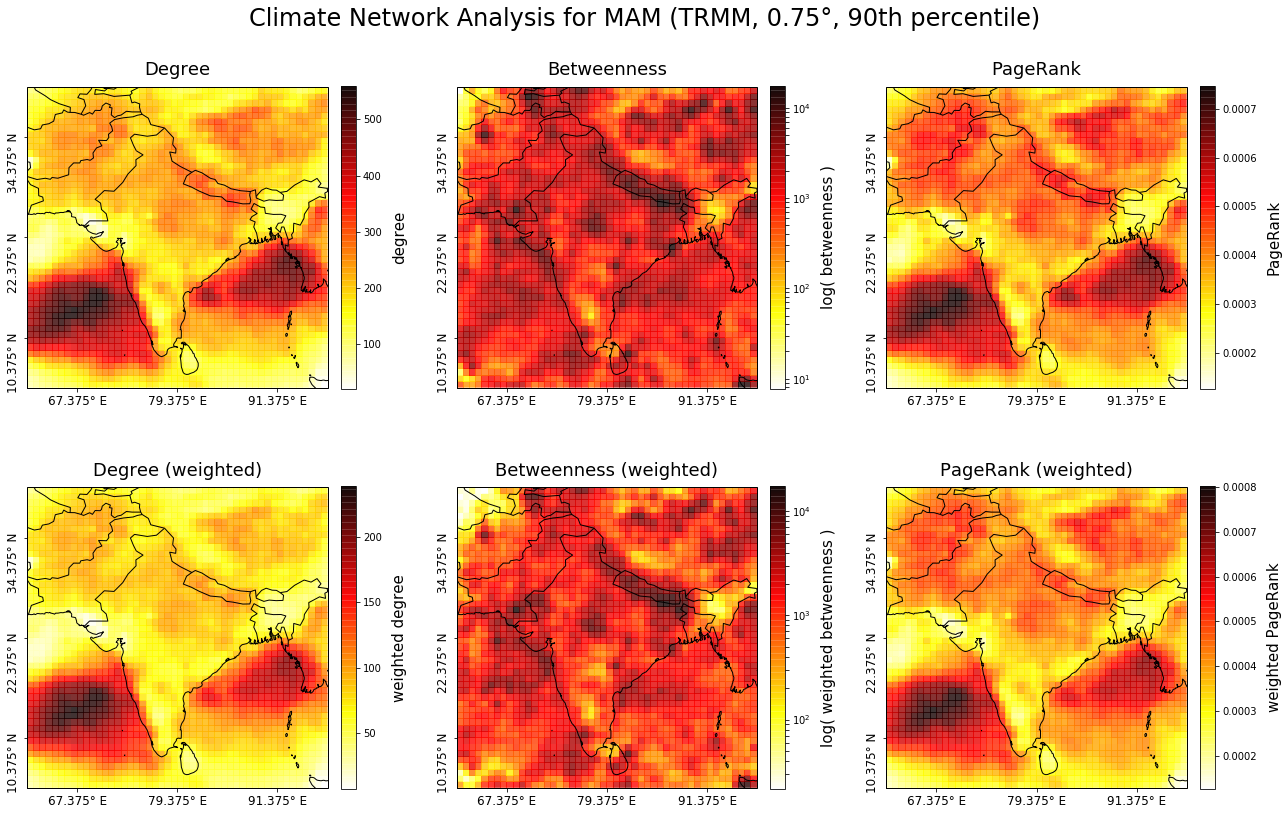
\includegraphics[width=\textwidth]{{./99_appendix/img/event_sync_0.75-0.9_MAM}.png}
  \caption{Weighted and unweighted degree, betweenness and PageRank for the pre-monsoon season (MAM). Based on the TRMM dataset at {0.75\degree} resolution.}
  \label{fig:results_mam}
\end{figure}

The degree is strongest over the Indian ocean, enframing the Indian subcontinent from both east and west. On the western side lies the Arabian Sea, over which an area of high degree extends from the far west up to the natural barrier of the Western Ghats mountain range (WG). A similar but smaller area over the Bay of Bengal to the east of the Indian subcontinent ranges from the Indian coast onto the lands of Myanmar (BoB). Further patches of significant degree can be found over the Tibetan Plateau (TP), over north-eastern India and Nepal at the brim of the Himalayas (Himalayas) and over areas of Pakistan and Afghanistan (NP, representing North-Pakistan).

The patterns in the betweenness are much less clear and conclusive. There are, however, still spots that display significantly high betweenness, especially the area over Nepal (Himalayas). Additionally, smaller patches of high betweenness are sprinkled over the Tibetan Plateau (TP), to the north of Pakistan and over central India.

During the pre-monsoon or "summer" season, rainfall in southern or central India is a rare occasion, as can be seen in \cref{apx:trmm_prec}. Temperatures during these hot summer months range around 30-40\degree Celsius (\cref{apx:era_t}), even causing drought-like conditions in some years. This coincides well with our findings that the most central parts of the network are located in big clusters over the Indian ocean: as the ocean temperatures are lower than the ones on the subcontinent, wind channels moisture away from the land and onto the ocean.

However, the degree of a location does not (necessarily) represent the amount of rainfall but the overall connectedness of a location in the network, which is harder to reason about. A location can obtain high degree centrality simply because it is part of many large-scale events like thunderstorms that cause high or even extreme precipitation in a large area, which would certainly explain the clusters over the ocean.

Furthermore, the significant degree and high betweenness at the brim of the Himalayas could be caused by its connectedness to either one or both clusters over the Indian ocean. As an area displaying high betweenness lies on a large portion of shortest paths in the network, a connection of the cluster over the Bay of Bengal to the Himalayas certainly makes sense. This would also be supported by the general importance of the Himalaya region as a "monsoon through" that serves as an entry point to the subcontinent for moisture from the Bay of Bengal (see \cref{c:ism_overview}).


\newpage
\subsection{Monsoon season (JJAS)}
[TODO: PageRank analysis once updated version is evaluated]

Analyzing the months of the primary monsoon season (JJAS, June-September) as shown in \cref{fig:results_jjas} yields somewhat unexpected results: degree and betweenness both display a strong but compact pattern over Northern Pakistan (NP). Further areas of significant degree are located on the Tibetan Plateau (TB) and over the Indian Ocean around the southern tip of India (Arabian Sea/WG and BoB).

\begin{figure}[h]
  \centering
  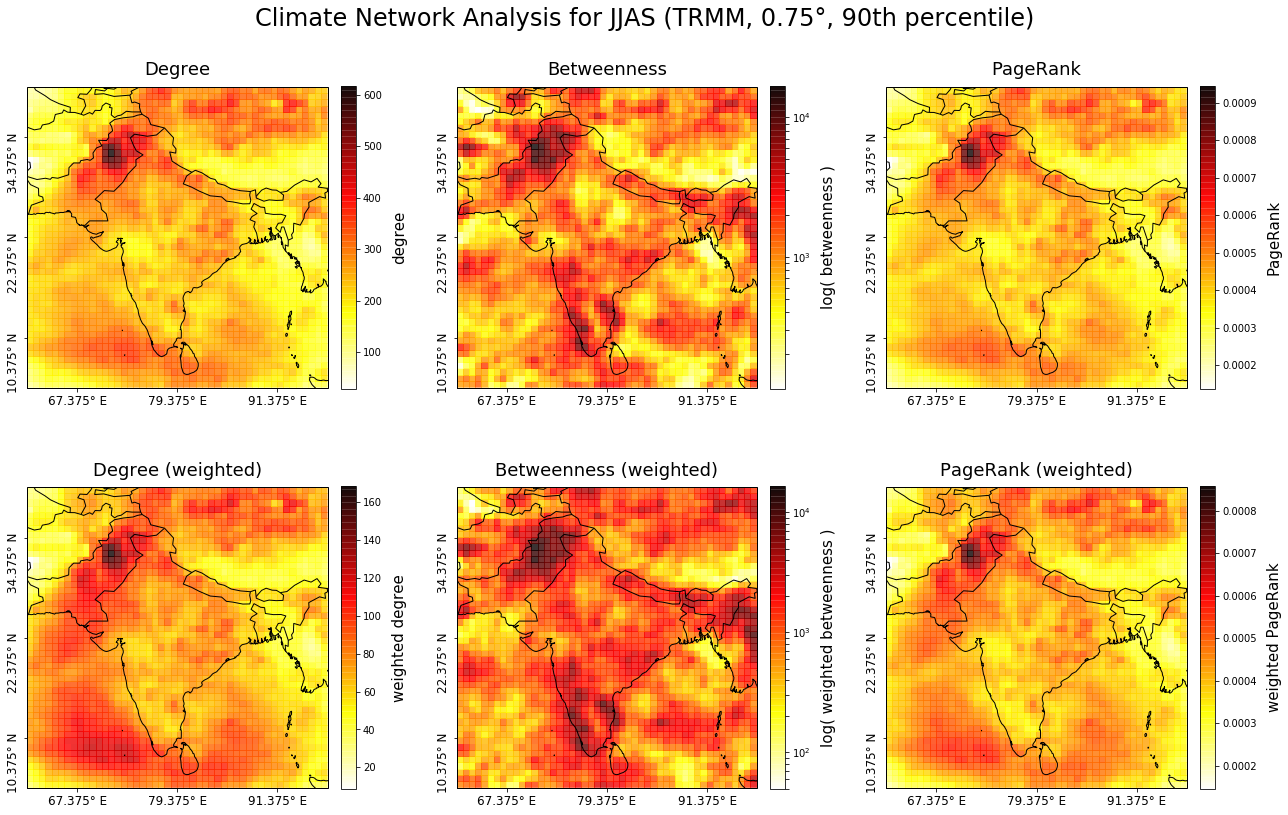
\includegraphics[width=\textwidth]{{./99_appendix/img/event_sync_0.75-0.9_JJAS}.png}
  \caption{Weighted and unweighted degree, betweenness and PageRank for the primary monsoon season (JJAS). Based on the TRMM dataset at {0.75\degree} resolution.}
  \label{fig:results_jjas}
\end{figure}

High betweenness can be seen over Northern Pakistan (NP), near the Western Ghats (WG) and Kerala as well as on the other side of the southern tip of India. Having locations of high degree and high betweenness clustered over a region like Northern Pakistan suggests that even such a small region can be a great influence to many parts of the Indian subcontinent. However, it is hard to reason where the region's importance stems from. Perhaps it serves as a pivot between the Tibetan Plateau, the Arabian Sea and central India and thus is part of many paths in the network.

The regions of strong betweenness flanking the Western Ghats could be explained by the important role of the Kerala region in the overall onset of the monsoon season. Kerala is typically the first region of the Indian subcontinent that is reached by monsoonal rainfalls. Thus, it can be argued that extreme events in Kerala tend to lead events on the mainland and are most probably connected to many locations in India. Furthermore, the jet coming from the Arabian Sea are split into two streams due to the heights of the Western Ghats. Continuing into the mainland, these two streams could be a cause for the patterns of high betweenness on either side of the Western Ghats.

\newpage
\subsection{Post-monsoon season (OND)}
[TODO: PageRank analysis once updated version is evaluated]

The post-monsoon season (OND, October-December) is typically also called the north-east monsoon. The unique characteristics of the north-east monsoon can be clearly identified based on the network measures as shown in \cref{fig:results_ond}.

\begin{figure}[h]
  \centering
  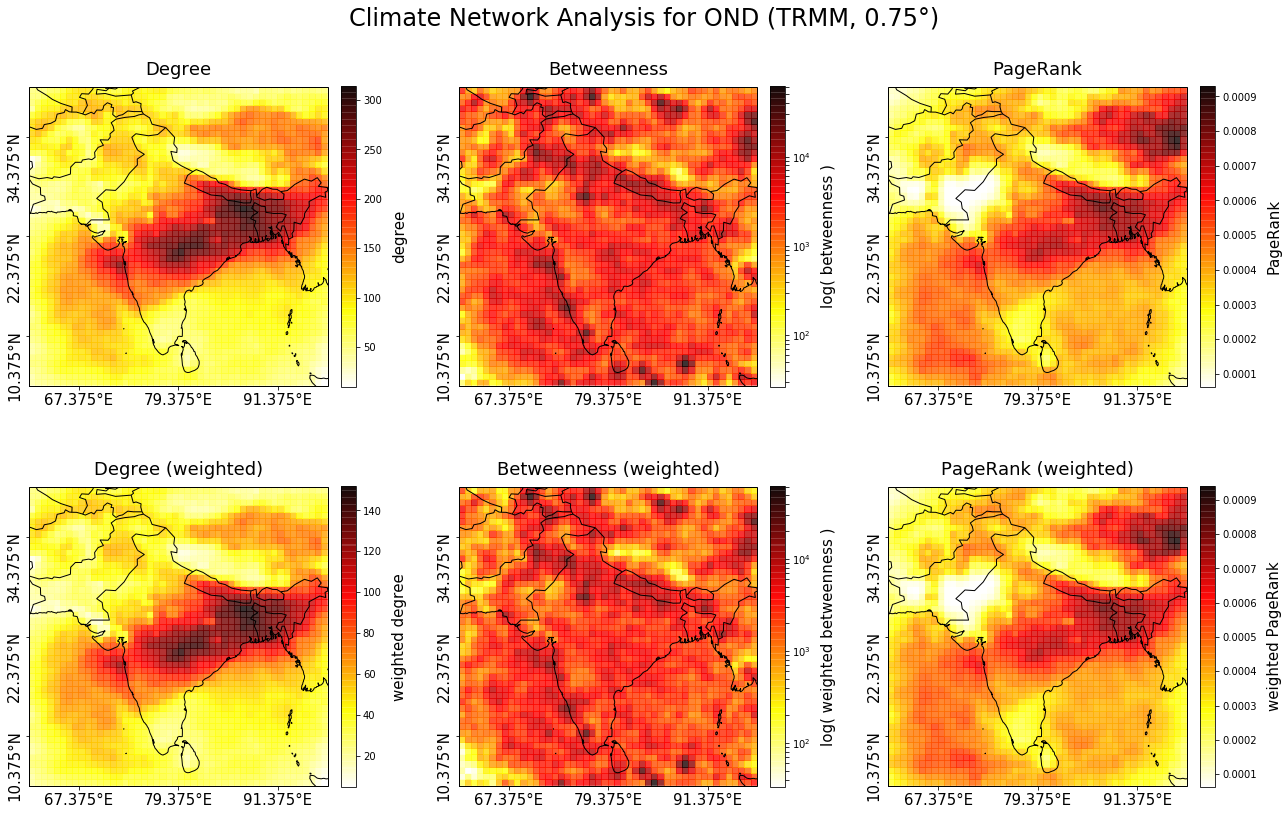
\includegraphics[width=\textwidth]{{./99_appendix/img/event_sync_0.75-0.9_OND}.png}
  \caption{Weighted and unweighted degree, betweenness and PageRank for the post-monsoon season (OND). Based on the TRMM dataset at {0.75\degree} resolution.}
  \label{fig:results_ond}
\end{figure}

 More specifically, a single area of very high degree encompasses entire central and north-eastern India, starting over the Arabian Sea (WG) and ranging well into Bangladesh. The degree in this area is at its highest over Nepal close to the Himalayas. The area further extends over the Tibetan Plateau (TP), although with less strength. Similarly, areas of high betweenness are located over Nepal, at the coast of the Arabian Sea, over North Pakistan (NP) and on the Tibetan Plateau (TP).

[TODO: interpretation]

\subsection{Intercomparison with \citet{Stolbova.2015}}
So far, we have strongly based our climate network analysis on the work of \citet{Stolbova.2015}, additionally evaluating PageRank measures and weighted networks. This section shows the results as they have been presented in the referred work and compares them to the results we have obtained from our analysis. Next to giving an indication about the validity of our approach, this might also show new properties that have only recently developed, as we have had access to four additional years of the TRMM dataset.

\begin{figure}[H]
  \centering
  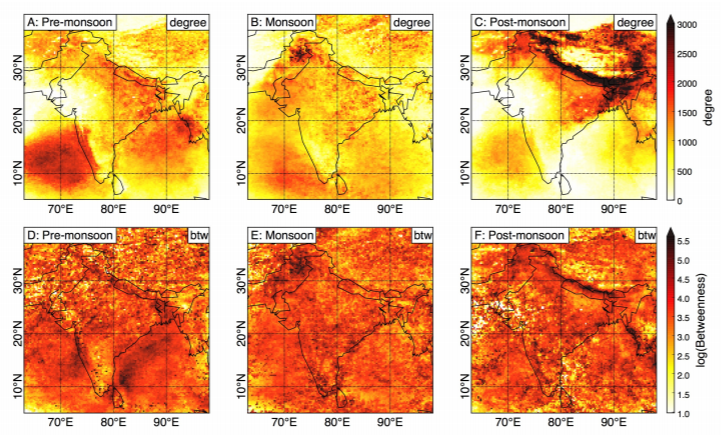
\includegraphics[width=\textwidth]{./99_appendix/img/results_stolbova.png}
  \caption{Degree and betweenness centrality as presented in \citet{Stolbova.2015}. Based on the years 1998-2012 from the TRMM dataset at {0.25\degree} resolution}.
  \label{fig:results_stolbova}
\end{figure}

The visualizations as shown in \cref{fig:results_stolbova} are obviously much more granular and detailed, as the full {0.25\degree} resolution was used for the climate network compoutations (and we have used a {0.75\degree} resolution). However, the general patterns seem to overlap well for the first two monsoon seasons. The main regions of interest during the pre-monsoon season are similarly located over the Arabian Sea, the Bay of Bengal, south of the Himalayas and on the Tibetan Plateau. The monsoon season shows the same strong clustering over North Pakistan and significant patterns at the southern tip of India as well as over the Arabian Sea.

Comparing the results for the post-monsoon season, we find that the discrepancies are much more significant. While the most central locations are clustered around the Himalayas in both \cref{fig:results_ond} and \cref{fig:results_stolbova}, the area of high degree extends much farther to the west in our results. Additionally, the results as shown in \cref{fig:results_stolbova} seem to be more concentrated to the Himalaya region and extend far up on the Tibetan Plateau.

We mainly attribute the observed discrepancies to one important factor: we have used a much lower resolution to be able to speed up computation of the synchronization matrix and climate networks. The full synchronization matrix for a {0.25\degree} resolution restricted to our area has a degree of 21609, making traversal of the matrix a computationally very complex effort (compared to the 2401 degree matrix using {0.75\degree} resolution). It is clearly visible that the higher resolution shows much more detail than our implementation. Furthermore, the choice of resolution might also have an impact on the general structure of a network, as a {0.25\degree} resolution results in a matrix that is much more sparse than it would be after aggregation.

% Furthermore, due to the lower resolution in our synchronization matrix, our implementation also differs in the threshold applied to the synchronization matrix. While the threshold was set to the 95th percentile in \citet{Stolbova.2015}, we used a lower threshold to get a network with a more meaningful amount of links. More specifically, we set the threshold to the 90th percentile, still only leaving the 10\% most significantly synchronous links. Especially

\section{Conclusion}
\label{st:event_sync_conclusion}
[TODO: conclude this chapter (summary, main takeaways)]

\chapter{Part 2: Prediction of Monsoon Onset}
\label{c:part2}
The onset of the ISM plays a crucial role in both the daily lives of the Indian population as well as regarding the Indian economy overall. Whether the ISM is a blessing or a curse mostly depends on the timing, strength and durability of monsoonal rainfalls. While we have analyzed the distribution of extreme rainfall events in the previous chapter, this chapter is fully dedicated to the problem of ISM onset prediction. We focus on the monsoon onset over Kerala (MoK), as it marks the beginning of the yearly monsoon season for the entire Indian subcontinent.

Our approach to predicting the ISM onset is based on neural networks and their training on spatiotemporal meteorological datasets. An example of such a dataset is the TRMM dataset we have introduced and used in the previous chapter. As the TRMM dataset is focused solely on precipitation, we have found that it is not well suitable for our prediction task: many locations do not receive rainfall at any given time, making the data very sparse. As an alternative dataset, we introduce the ERA-Interim dataset in the first part of this chapter (\cref{st:era_interim}). The ERA-Interim dataset provides many more features (e.g., temperature), many of which are less sparse, making them more suitable as training data for our models.

The neural network architecture we have found to work best is based on a new layer that has been introduced relatively recently. This new layer, the ``ConvLSTM'' layer, is based on a combination of convolutional and recurrent neural network concepts. We shortly introduce the main characteristics of ConvLSTM layers in \cref{sst:neural_networks}. Following up in \cref{st:nn_implementation}, we introduce the architecture of our final neural network model and present the experiments we have performed for its evaluation. We also provide an overview of the other model architectures we have tried but not developed further, as their accuracy was subpar.

\section{The ERA-Interim Dataset}
\label{st:era_interim}
The ERA-Interim dataset is a global atmospheric reanalysis product created by the ECMWF. The center had already produced the popular ERA-40 reanalysis until 2002 and, during this process, had identified several issues in data assimilation that they addressed with the creation of the ERA-Interim reanalysis. ERA-Interim is also thought as a ``bridge'' between ERA-40 and a future reanalysis that spans the entire 20th-century \citep{Dee.2011b}.

Generally speaking, a reanalysis product is a dataset that provides many meteorological features through a single framework, for the same locations, and at the same resolution. Most often, reanalysis products are available on a global scale, which also holds true for ERA-Interim. The features provided by reanalysis datasets are not purely based on real observations, as this would often be unfeasible for the high spatial and temporal resolutions required. Instead, the features are based on complex data assimilation algorithms and a combination of observations, simulations, and forecasts.

The ERA-Interim reanalysis provides hundreds of features for locations all around the world. ERA-Interim is available starting in 1979 and continues to be produced, albeit with a two-month delay. The native spatial resolution of the dataset is equal to approximately {0.75\degree} on a geographical coordinate system.

To achieve consistency and comparability with the TRMM dataset, we subset the global ERA-Interim reanalysis into a gridded area between 4.5-40.5\degree N and 61.5-97.5\degree E. While this is slightly smaller compared to the area we have extracted from TRMM, the TRMM dataset shrinks to equal dimensions after the aggregation algorithm is applied (4.375-40.375\degree N, 61.375-97.375\degree E). After the described aggregation of the TRMM dataset, the two datasets are both in a {0.75\degree} resolution. The final coordinate systems are offset by 0.125\degree, which is inherent to the datasets themselves.

While the ERA-Interim reanalysis provides a multitude of features, we focus on only a handful of features in this work. More specifically, we extract the temperature and relative humidity at a 1000hPa pressure level, the U and V components of wind at 700hPa and the U-component of wind at 200hPa. An overview of the extracted features is shown in \cref{tab:era_features}, along with the corresponding identifiers we use later on. \cref{apx:era_features} additionally shows the development of the most important features over the course of the pre-monsoon season.

\begin{table}[h!]
  \centering
  \begin{tabular}{rl}
    \toprule
    \textbf{ID} & \textbf{Description} \\
    \midrule
    \textbf{msl} & Mean-Sea Level Pressure \\
    \textbf{r} & Relative Humidity at 1000hPa \\
    \textbf{t} & Temperature at 1000hPa \\
    \textbf{u700} & U-Component of Wind at 700hPa \\
    \textbf{v700} & V-Component of Wind at 700hPa \\
    \textbf{u200} & U-Component of Wind at 200hPa \\
    \bottomrule
  \end{tabular}
  \caption{List of features from ERA-Interim and their identifiers as used in this work.}
  \label{tab:era_features}
\end{table}

\section{Related Work}
Many of our experimental models are based on a relatively new approach to training neural networks on spatiotemporal data. We specifically refer to the work of \citet{Shi.2015}, where a newly defined \textit{ConvLSTM} neural network layer was first applied to precipitation forecasting. Due to the reliance of many of our models on these layers, \cref{sst:neural_networks} is thought to provide intuition about the applicability of ConvLSTM networks. For the remainder of this work, we assume that the reader is familiar with neural network principles. However, as convolutional and recurrent layers are what ConvLSTM layers are based on, we explain some of their characteristics along the way.

\subsection{Convolutional recurrent neural networks}
\label{sst:neural_networks}
ConvLSTM networks as introduced by \citet{Shi.2015} were originally applied to the problem of precipitation nowcasting, the primary goal of which is described as giving a ``precise and timely prediction of rainfall intensity in a local region over a relatively short period of time (e.g., 0-6 hours)'' \citep{Shi.2015}. In the aforementioned work, the authors try to predict a sequence of future precipitation radar maps from a sequence of past radar maps, essentially performing sequence-to-sequence prediction. These kinds of prediction tasks based on spatiotemporal data (where time, as well as geographical location, needs to be accounted for) are challenging, as a suitable neural network needs to be able to handle very high input and output dimensionalities.

An approach that is often used for sequence-to-sequence prediction is a two-layer architecture in which a first Long-Short Term Memory (LSTM) network reduces the input into a fixed-length sequence (``encodes'' the input into an internal representation), while a second LSTM network then predicts an output sequence using as input the fixed-length sequence (``decoding''). This encoder-decoder framework was originally described in \citet{Sutskever.2014} and has been applied to many sequence-to-sequence tasks like machine translation. However, \citet{Shi.2015} have found that the LSTM networks used for regular sequence-to-sequence prediction are not well suited to process spatiotemporal data. While they also use an encoding-decoding pattern in their models, \citet{Shi.2015} propose a new type of network layer based on LSTM layers that can better take into account the spatial dimension of input values.

The newly proposed ConvLSTM network layer combines the concept of convolutions as applied in convolutional networks with the internal structure of regular LSTM layers. In a ConvLSTM network, the states in each LSTM-cell are represented by 3D-tensors with the same spatial dimensions as the input data. Updates to any hidden state are then performed by applying convolutions to both the input values and the previous state, meaning that the new state of any location is based on the previous and current values of its immediate neighbors \citep{Shi.2015}.

\begin{figure}[h!]
  \centering
  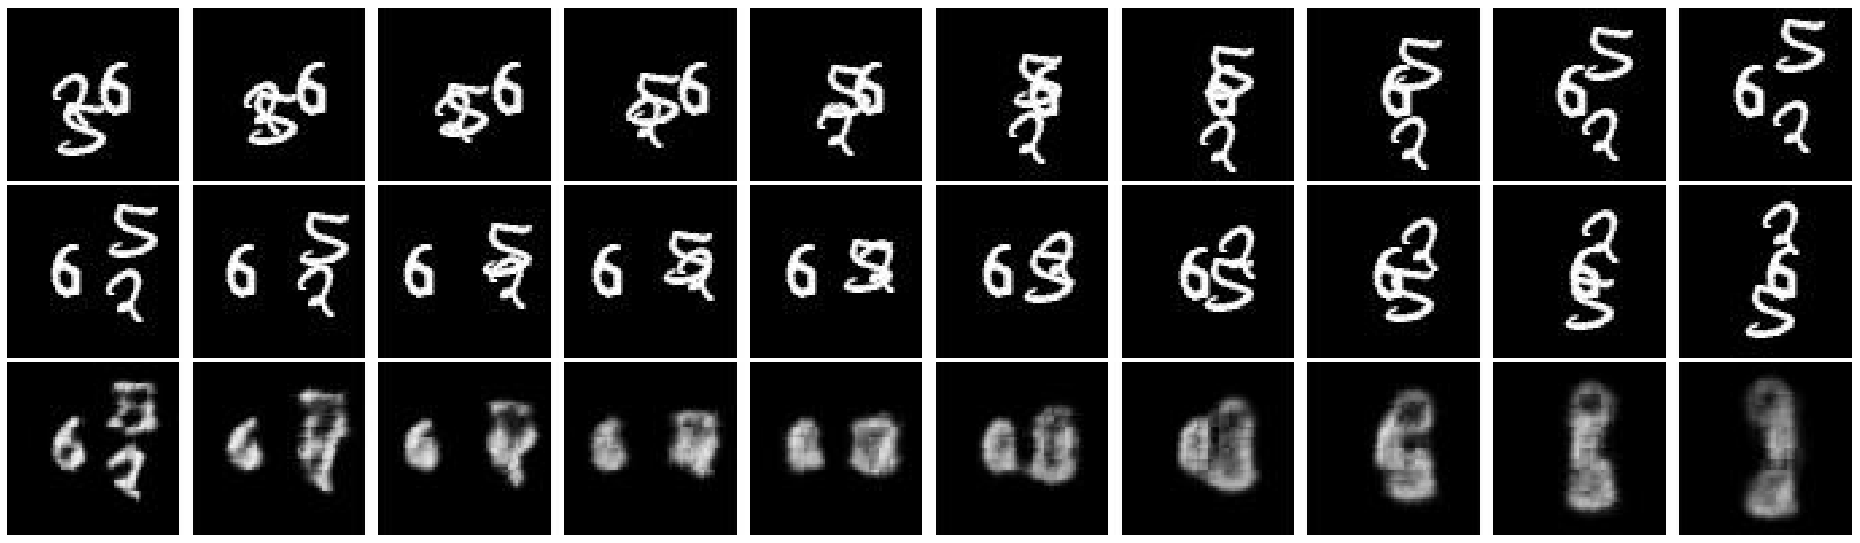
\includegraphics[width=0.7\linewidth]{./99_appendix/img/conv_lstm_predictions}
  \caption{Results of predicting an ``out-of-domain'' moving-digits problem using ConvLSTM networks as depicted in \citet{Shi.2015}. From top to bottom: input frames, ground truth and predictions.}
  \label{fig:conv_lstm_predictions}
\end{figure}

Based on the previously mentioned encoding-decoding pattern and their new ConvLSTM network layers, \citet{Shi.2015} have built several models and evaluated them on both a generated dataset with moving digits (as shown in \cref{fig:conv_lstm_predictions}) as well as on a real radar map dataset. Over both of these evaluations, the ConvLSTM architecture outperformed a fully-connected regular LSTM architecture by a significant margin. Additionally, while the contours of the precipitation predictions were found to be blurred, they still significantly outperformed the benchmark concerning overall precision \citep{Shi.2015}.

\section{Prediction of Monsoon Onset using Neural Networks}
\label{st:nn_implementation}
Looking to find a model capable of learning the patterns leading up to the monsoon onset, as well as predicting the onset itself, we evaluated many different approaches to training neural networks based on spatiotemporal meteorological datasets like TRMM and ERA-Interim. Each approach had its advantages and disadvantages, many of which we only learned through trial and error and subsequently used to build improved architectures. Over many iterations with vastly different model architectures, we finally got to a model that seems to be able to learn patterns present before the monsoon onset and, based on these patterns, predict the monsoon onset with reasonable accuracy.

The first part of this section is thus focused on our certainly most important and useful result: our final working models and their evaluation. We describe their general architecture as well as the different evaluation schemes and parameters we have used. Furthermore, we evaluate how well the models have performed over the entirety of our experiments and assess the prediction capabilities from different points of view (e.g., how accurately can we predict on the 15th of May, or how accurately can we predict ten days before onset).

That being said, we would probably not have gotten to our final models without having tried many other architectures beforehand, iteratively improving upon the findings of each. The remainder of this chapter is then dedicated to a brief overview over all the model architectures we have evaluated during the creation of this work (in chronological order), along with a summary of our most important findings during the process.

\subsection{E4: A working model based on ERA-Interim}
\label{sst:final_model}
The neural network architectures and hyperparameter tunings that we have found to work best during our experiments are based on two main ingredients: the ERA-Interim dataset with several of its features and multiple stacked convolutional recurrent layers (ConvLSTM2D). These models are all based on the latest Keras 2.0 and Tensorflow 1.4 Python libraries, which have greatly simplified our development, as even the relatively new ConvLSTM2D layer type is already implemented and usable from within the core libraries. The remainder of this section is dedicated to a more detailed description of the way we preprocessed the ERA-Interim dataset and built our final working model architecture. This specific model architecture is further also referred to as \textit{E4}, the reasons of which will be explained later on.

\subsubsection{Data preprocessing}
One of the most important steps during the process of creating a neural network model (or any other machine learning model at that) is the preparation of the data that is to be used as its foundation. Without properly formatted input data, a neural network will typically not be able to learn any meaningful patterns. Over the course of our experiments, we tried different datasets (TRMM and ERA-Interim) and, more importantly, many heterogenous input formats, of which each had its advantages and disadvantages (we go over all of these evaluated input formats in their respective sections).

The approach we use in our final model architecture (E4) is most easily explained through an example: given time series data before the monsoon onset in an arbitrary year, we extract a fixed-length sequence (for example, a sequence of 60 consecutive days). The sequence ends at a given distance before the onset (e.g., 14 days before) and starts 60 more days before that. Feeding this sequence (corresponding to a single training example) to our neural network model after training, we would like it to predict the number 14, which is comparable to a simple regression task. Intuitively, we ask our model the following question: "given data from the last 60 days, in how many days from today will the monsoon arrive?".

The actual preprocessing of the ERA-Interim dataset is slightly more complex: instead of a simple time series from which a sequence is extracted, we have a time series where each timestep is represented by a multidimensional matrix (a \textit{3D-tensor} as shown in \cref{fig:e4_tensor}). For each location in the ERA-Interim coordinate grid as well as for each feature used from ERA-Interim (e.g., temperature), these tensors contain the value of the respective feature at the respective location (at that timestep).

\begin{figure}[h!]
  \centering
  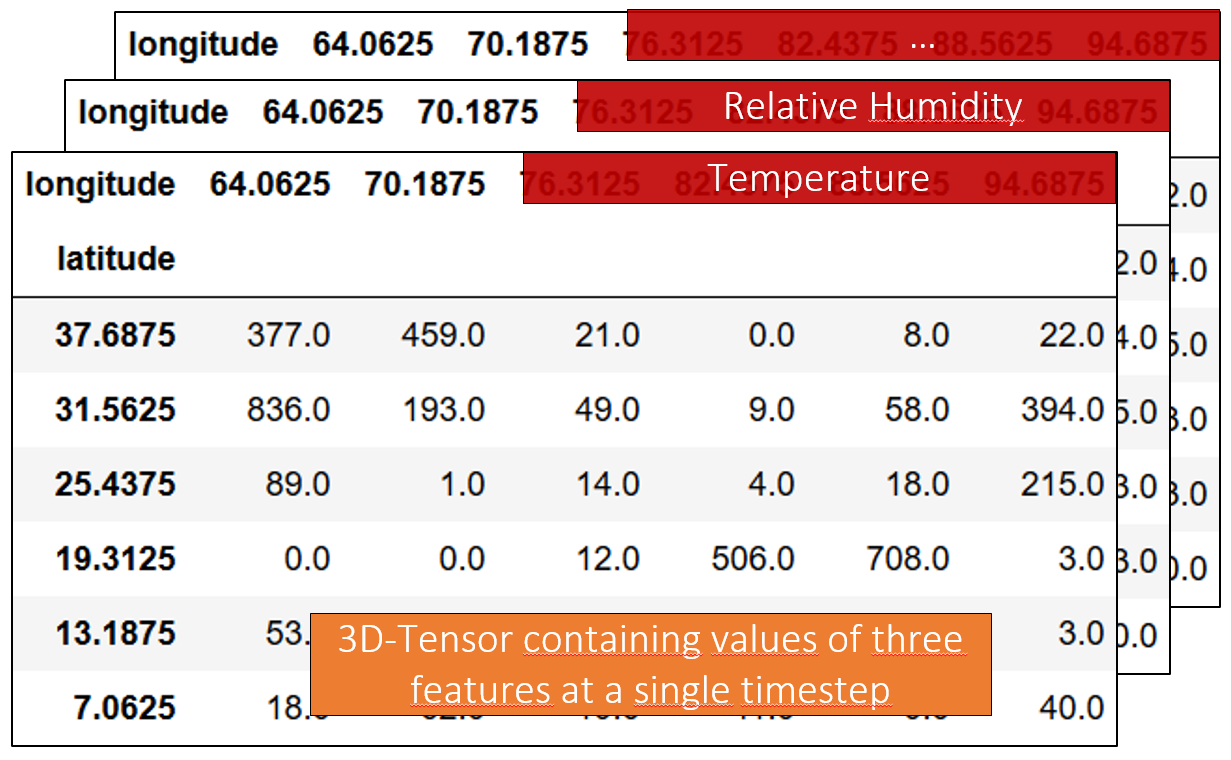
\includegraphics[width=0.6\linewidth]{./99_appendix/img/E4_tensor}
  \caption{A single timestep as extracted from a training sequence. The 3D-tensor contains several features from ERA-Interim and, for these features, values at each location.}
  \label{fig:e4_tensor}
\end{figure}

If we were to train our model only based on sequences that end 14 days before the onset, it would most certainly always predict the number 14, no matter the actual input. To train our model for different distances, we need to repeat the sequence extraction process many times per year, using a different distance to the monsoon onset in each repetition. Our most successful models are based on 30 training examples per year with distances in the range of $[1, 30]$ and a sequence length of around two months. In such a case, one of the training examples of each year ends one day before the respective onset ($t-1$) and consists of the days until $t-60$. A second training example ends at $t-2$ and starts at $t-61$, while a third training sequence ranges from $t-3$ to $t-62$. This is repeated up to a training example with data in the range of $t-30$ to $t-89$, yielding, in total, 30 training examples per year. This process is more intuitively shown in \cref{fig:e4_preprocessing}.

\begin{figure}[h!]
  \centering
  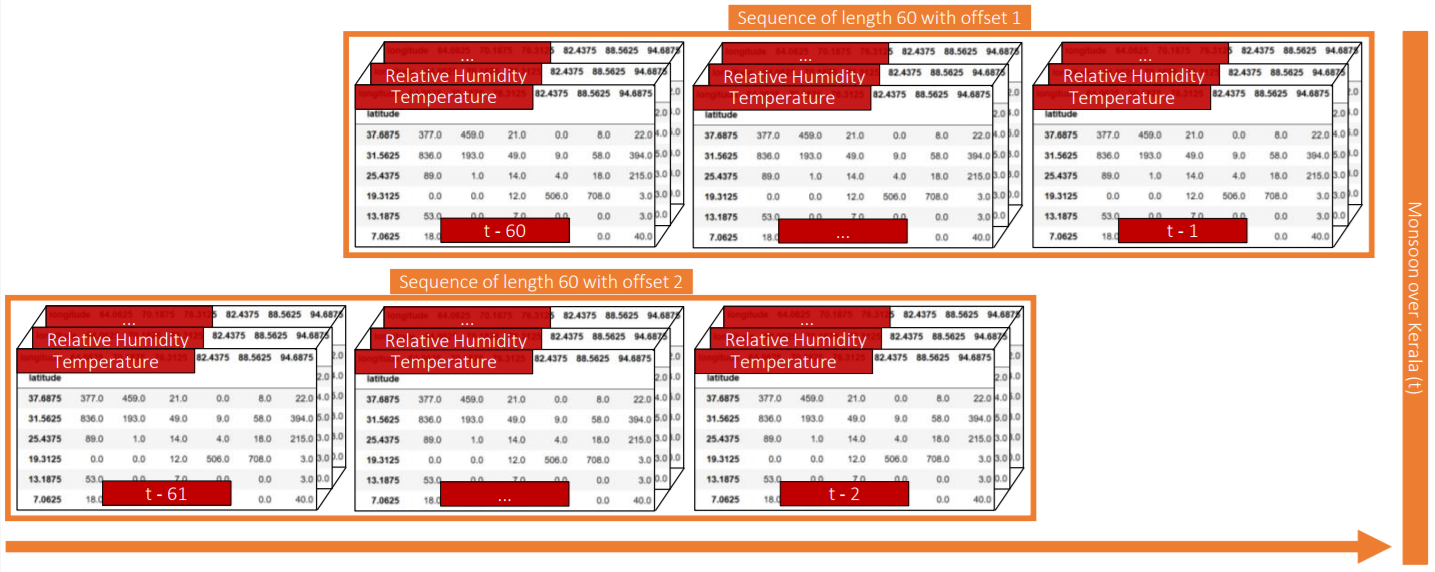
\includegraphics[width=\linewidth]{./99_appendix/img/E4_preprocessing}
  \caption{Two exemplary training examples based on three ERA-Interim features and a sequence length of 60 days. One training example consists of 60 timesteps, each of which is represented by a 3D-tensor as shown in \cref{fig:e4_tensor}.}
  \label{fig:e4_preprocessing}
\end{figure}

\paragraph{Normalization} An additional step during data preprocessing is often the normalization of data into consistent ranges. Even though neural networks could learn without normalization, it often improves and speeds up their learning process. If different input features do not adhere to the same distribution (e.g., temperature and rainfall), the different magnitudes can lead to problems during the optimization process (when multiplying with the learning rate).

When processing the ERA-Interim dataset into a training, validation and test set, we apply statistical z-score standardization to center the mean of each feature at each location separately. To prevent the introduction of any bias, the mean and standard deviation of the training set are reused when normalizing the values in the validation and test sets. This means that, to calculate the standardized value of feature $f$ at location $x$/$y$ in some timestep of a test sequence, the mean of said feature at said location over the training set would be subtracted, after which the result would be divided by the corresponding standard deviation.

\subsubsection{Model architecture}
It is not hard to see that a single ERA-Interim coordinate grid is inherently similar to a simple multichannel image: we have a height (latitudes), a width (longitudes) and multiple channels (e.g., temperature and relative humidity). When working with images, convolutional neural networks are by far the most prevalent approach. They have led to great progress in image recognition and other domains. However, 2D-convolutions are not directly applicable to multiple images ordered in a sequence (like a movie). Instead, they first need to be combined with recurrent network structures like LSTM.

We have already introduced a recent approach to the problem of learning from spatiotemporal data: the ConvLSTM2D neural network layer (\cref{sst:neural_networks}). In our case, this layer performed much better than a simple stacking of convolutional and recurrent layers, making it the most important part of many of our models (including E4). With ConvLSTM2D at its core, the E4 model architecture learns by processing input sequences as shown in \cref{fig:e4_preprocessing} using multiple ConvLSTM2D layers. From the sequence that these recurrent layers predict, the last state is flattened and passed through multiple fully-connected layers, the last one of which only consists of a single neuron. The network, therefore, predicts a single number, which intuitively corresponds to a regression model.

As an optional addition to the model, several time-distributed layers can be added in front of the core ConvLSTM2D layers. These time-distributed layers can apply any layer to a sequence and do so separately for each timestep in the sequence. For example, applying time-distributed Conv2D layers to a sequence of images would lead to a separate Conv2D layer with separate weights for each image in said sequence. We can use these time-distributed layers to apply additional convolutional and pooling layers before feeding the sequences into the recurrent layers, adding further feature detection and dimensionality reduction capabilities.

An exemplary model based on the described architecture is shown in \cref{fig:e4_architecture}. Let us assume that the model therein has already been trained appropriately and is now used to perform a prediction on a single test example. The model passes this test example through two time-distributed layers consisting of Conv2D layers, each of which applies a 3x3 convolutional kernel and 16 filters (separately for each tensor in the input sequence). A further time-distributed layer applies a MaxPool2D layer, independently reducing each tensor in the input sequence to half its original spatial dimensions. The pooled sequences are passed through three ConvLSTM2D layers, each also with 16 filters and a 3x3 convolutional kernel applied to the state transitions. The last state of the final ConvLSTM2D layer (a single tensor) is flattened and passed through three 1024-neuron dense layers that are activated with the ReLU function, after which a linearly activated single-neuron layer outputs a numerical prediction.

\begin{figure}[h!]
  \centering
  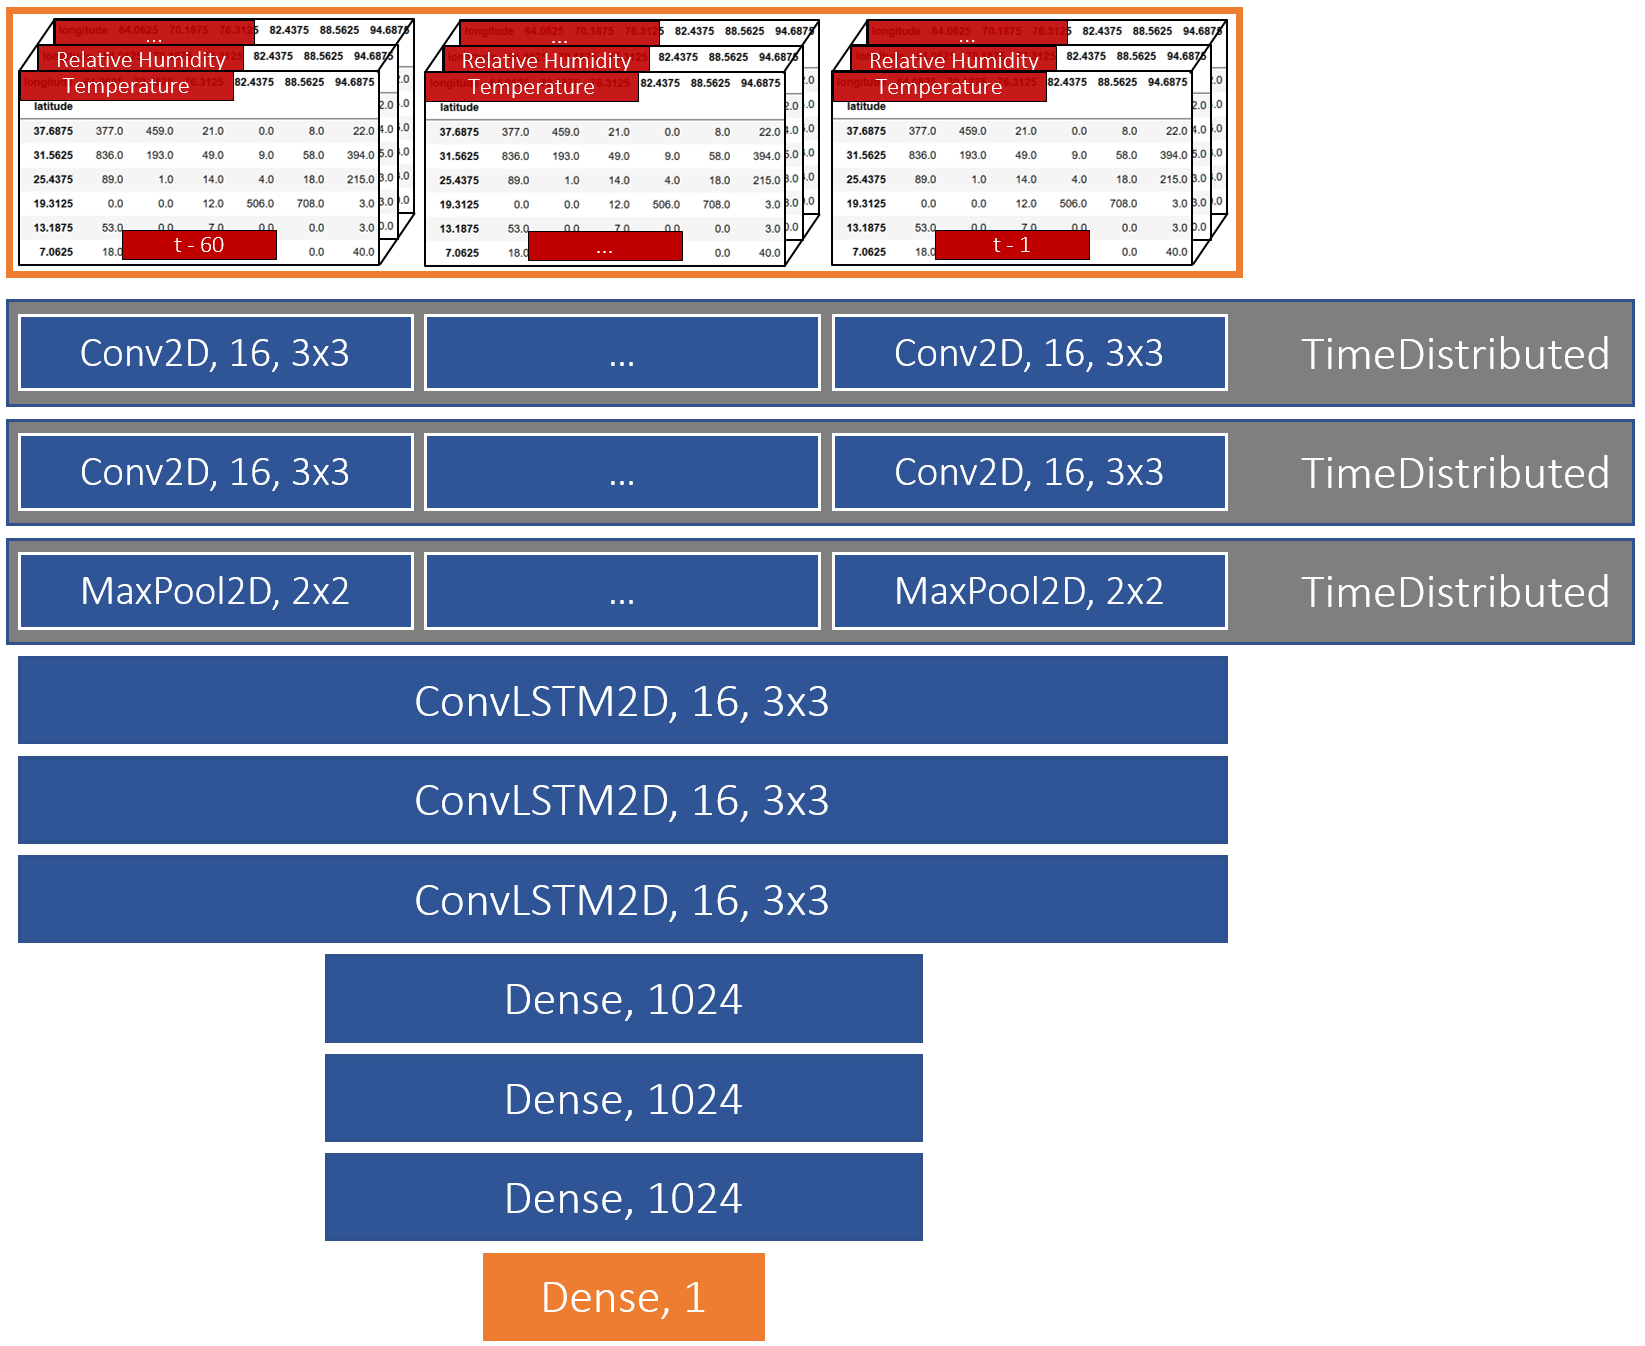
\includegraphics[width=0.9\linewidth]{./99_appendix/img/E4_architecture}
  \caption{Exemplary model architecture of the E4 class (corresponding to the architecture used in EV07 and EV12 as introduced later on). An input sequence (e.g., a test example) with a structure as shown in \cref{fig:e4_preprocessing} is passed through the different layers of the model and used to perform a numerical prediction using a linearly activated single-neuron output layer.}
  \label{fig:e4_architecture}
\end{figure}

\paragraph{Regularization} To reduce the tendency of the model to overfit to the training set, we apply L2-regularization to the kernels of all types of layers (Conv2D, ConvLSTM2D, Dense). This increases the loss whenever the model's internal representation of the problem gets too complex, effectively improving its ability to generalize. Also, we can and do most often use dropout after each layer. However, the exact regularization and dropout parameters vary with each tuning.

\paragraph{Batch normalization} To speed up the training of our models, we make use of batch normalization after each layer in the models. During the training process, a batch normalization layer normalizes (``centers'') the activations of each batch of training examples, preventing even small initial shifts in batch statistics (``internal covariate shift'') to grow increasingly large when processed by many subsequent layers in a deep network.

\subsubsection{Model evaluation}
On our search for the best configuration to train our models with, we performed 45 experiments for this final model architecture alone. The parameter space we were searching through can be split into two major categories: ``hyperparameters'', referring to the parameters that are typically heavily tuned to improve model performance (e.g., learning rate, dropout rates, kernel sizes, etc.), and a second category that is more fundamental, as it already influences the data when it is being preprocessed. The choice of datasets and features thereof (see \cref{st:era_interim}), as well as the amount of data that is being fed to the model (e.g., the sequence length), are exemplary parameters that we assign to the latter category. An overview of such ``meta-hyperparameters'' is shown in \cref{tab:meta_parameters}.

\begin{table}[h!]
  \centering
  \begin{tabular}{|r|c|c|c|c|c|c|}
    \hline
    \textbf{ERA-Features} & \multicolumn{1}{c|}{msl/r/t} & \multicolumn{2}{c|}{msl/r/t/u700/v700} & \multicolumn{3}{c|}{msl/r/t/u700/v700/u200} \\
    \hline
    \textbf{Onset Dates} & \multicolumn{3}{c|}{IMD (1979-2017)} & \multicolumn{3}{c|}{Objective (1979-2007) + IMD (2007-2017)} \\
    \hline
    \textbf{Sequence Length} & 32 & 42 & 47 & 62 & 77 & 92 \\
    \hline
    \textbf{Sequence Offset} & 0-8 & 0-21 & 0-22 & 5-25 & 0-30 & 1-30 \\
    \hline
  \end{tabular}
  \caption{``Meta-hyperparameters'' as they have been used in the final E4-class models. IMD onset dates until 2007 are extracted from \citet{Singh.2009} and concatenated with official IMD dates (2007-2017). Objective onset dates are extracted from the same source, but then also concatenated with IMD dates. The Sequence Offset specifies the range of offsets that is generated (meaning that for a value of 1-30, 30 examples are generated for each year with the smallest distance to the onset being 1 day). Details about the listed ERA-Features can be found in \cref{tab:era_features}. }
  \label{tab:meta_parameters}
\end{table}

\paragraph{Training, validation and test set}
The ERA-Interim dataset was split into three fixed sets for each of our experiments: a training, validation and test set. As can be seen in \cref{tab:train_test_split}, we originally started with only three years in the validation and five years in the test set (out of 38 years). When many models seemed to fit the training set very well, we decided to reduce the size of the training set, extending both the validation and test set (to four and eight years, respectively).

Because the ``objective'' onset dates are extracted from two different distributions (data that follows the objective definition of \citet{Singh.2009} is available until 2007, after which the dates stem from the IMD), model performance was much worse when training on objective onset dates using the second split. After it was reduced to the years 1979-2005, the training set did no longer contain any years based on the official IMD dates, while most of the validation and test set were based on these IMD dates. The entire training set was thus based on one distribution, while most of the validation and test years were based on another distribution. Unsurprisingly, the overall strongest overfitting was observed in the few experiments that were carried out this way.

As a remedy to the previously mentioned problem, we devised a third split scheme with a more appropriate distribution of years for experiments on both IMD and objective onset dates. This third split scheme was created by choosing a random year from each decade before the year 2000, and three years from each decade after the year 2000, without previous evaluation or analysis. The scheme was then successfully applied to the remainder of the experiments, allowing to train and compare models based on both IMD and objective onset dates.

\begin{table}[h!]
  \centering
  \begin{tabular}{rccc}
    \toprule
    & \textbf{Split 1} & \textbf{Split 2} & \textbf{Split 3} \\
    \midrule
    \textbf{Training} & 1979-2009 & 1979-2005 & 79/81-84/86-89/91-94/96-99/01-02/06-09/11-13 \\
    \textbf{Validation} & 2010-2012 & 2006-2009 & 80/90/00/10/16 \\
    \textbf{Test} & 2013-2017 & 2010-2017 & 85/95/03/04/05/14/15/17 \\
    \midrule
    \textbf{Experiments} & 0-27 & 28-31 & 32-45 \\
    \bottomrule
  \end{tabular}
  \caption{The three different splits that have been applied to the dataset in the experiments for E4. Split 1 consists of 31 training years, 3 validation years and 5 test years. Split 2 consists of 27 training years, 4 validation years and 8 test years. The final split, Split 3, consists of 26 training years, 5 validation years and 8 test years, corresponding to 67\%/13\%/20\% of the overall years.}
  \label{tab:train_test_split}
\end{table}

\paragraph{Evaluation schemes}
Over the course of our experiments, we used various combinations of the previously described ``meta-hyperparameters'' (see \cref{tab:meta_parameters}), leading to what can be called \textit{evaluation schemes}. An evaluation scheme is a group of experiments that are based on the same high-level parameters but have been tuned using different hyperparameters. We can reduce the total of our 45 experiments to 17 such evaluation schemes, each consisting of one to nine experiments. The listing in \cref{tab:evaluation_schemes} shows these 17 evaluation schemes along with their ``meta-hyperparameters''. We regularly refer to these evaluation schemes in the remainder of this work.

\begin{table}[h!]
  \centering
  \begin{tabular}{cccccc}
    \toprule
    \textbf{ID} & \textbf{ERA-Features} & \textbf{Onset Dates} & \textbf{Seq. Length} & \textbf{Seq. Offset}  & \textbf{\#} \\
    \midrule
    EV01 & msl/r/t & IMD & 47 & 1-30 & 1 \\
    EV02 & msl/r/t & IMD & 62 & 1-30 & 2 \\
    EV03 & msl/r/t & IMD & 77 & 1-30 & 1 \\
    EV04 & msl/r/t & Objective+IMD & 62 & 5-25 & 3 \\
    EV05 & msl/r/t & Objective+IMD & 62 & 0-30 & 3 \\
    EV06 & msl/r/t & Objective+IMD & 62 & 1-30 & 3 \\
    EV07 & msl/r/t/u700/v700 & IMD & 62 & 1-30 & 9 \\
    EV08 & msl/r/t/u700/v700 & Objective+IMD & 32 & 0-30 & 1 \\
    EV09 & msl/r/t/u700/v700 & Objective+IMD & 62 & 0-21 & 3 \\
    EV10 & msl/r/t/u700/v700 & Objective+IMD & 62 & 0-22 & 8 \\
    EV11 & msl/r/t/u700/v700 & Objective+IMD & 62 & 0-30 & 3 \\
    EV12 & msl/r/t/u700/v700 & Objective+IMD & 62 & 1-30 & 2 \\
    EV13 & msl/r/t/u700/v700 & Objective+IMD & 62 & 0-8 & 3 \\
    EV14 & msl/r/t/u700/v700 & Objective+IMD & 92 & 0-30 & 1 \\
    EV15 & msl/r/t/u700/v700/u200 & Objective+IMD & 42 & 0-30 & 1 \\
    EV16 & msl/r/t/u700/v700/u200 & Objective+IMD & 62 & 0-30 & 1 \\
    \midrule
    \multicolumn{5}{r}{\textbf{Total number of experiments}} & 45 \\
    \bottomrule
  \end{tabular}
  \caption{Evaluation schemes for the E4-class models and the corresponding number of experiments, based on the ``meta-hyperparameters'' as shown in \cref{tab:meta_parameters}. Details about the ERA-features can be found in \cref{tab:era_features}.}
  \label{tab:evaluation_schemes}
\end{table}

\paragraph{Experimental conditions}
The experiments were run in different environments and are explicitly marked as such: either on a local GPU, the Kraken cluster or a Paperspace\footnote{https://www.paperspace.com/} virtual machine. \cref{tab:experimental_environments} provides a more detailed overview of the environments used during the experimental phase. While all of the experiments for the E4-class of models were run on the \textit{PS} environment due to performance constraints, most earlier experiments were run locally or on Kraken.

\begin{table}[h!]
  \centering
  \begin{tabular}{ ccc }
    \toprule
    \textbf{Environment} & \textbf{Trained on} & \textbf{Available memory} \\
    \midrule
    Kraken & CPU (24-cores) & 128GB RAM \\
    Local & GPU (GTX 970) & 32GB RAM, 4GB GPU \\
    Paperspace & GPU (Quadro P5000) & 30GB RAM, 16GB GPU \\
    \bottomrule
  \end{tabular}
  \caption{Runtime environments for the deep learning experiments.}
\label{tab:experimental_environments}
\end{table}

\subsubsection{Intermediary evaluation results}
To provide a better overview of the outcome of our experiments, we reduce the results presented to only the best experiment of any given evaluation scheme (i.e., its best performing ``hyperparameter tuning''). \cref{tab:evaluation_scheme_results} shows the loss and validation loss after some key epochs as well as after the final epoch. Notice that loss and validation loss measures are based on the mean-squared error (MSE) but tend to be higher due to the regularization that is additionally applied.

\begin{landscape}
  \begin{table}[h!]
    \centering
    \begin{tabular}{cccccccccccc}
      \toprule
      \textbf{Epoch} & \multicolumn{2}{c}{\textbf{10}} & \multicolumn{2}{c}{\textbf{30}} & \multicolumn{2}{c}{\textbf{50}} & \multicolumn{2}{c}{\textbf{100}} & \multicolumn{3}{c}{\textbf{Final}}\\
      & \textbf{Loss} & \textbf{Val. Loss} & \textbf{Loss} & \textbf{Val. Loss} & \textbf{Loss} & \textbf{Val. Loss} & \textbf{Loss} & \textbf{Val. Loss} & \textbf{Loss} & \textbf{Val. Loss} &  \textbf{Epoch Nr.} \\
      \midrule
      \textbf{EV01} & 48 & 132 & 37 & 85 & 30 & 87 & 15 & 72 & 11 & 68 & 500 \\
      \textbf{EV02} & 43 & 92 & 33 & 70 & 25 & 73 & 13 & 57 & 6 & 63 & 500 \\
      \textbf{EV03} & 54 & 76 & 35 & 63 & 24 & 87 & 14 & 96 & 6 & 69 & 500 \\
      \textbf{EV04} & 43 & 73 & 32 & 40 & 24 & 36 & 13 & 56 & 6 & 17 & 500 \\
      \textbf{EV05} & 69 & 86 & 41 & 54 & 25 & 45 & 17 & 26 & 12 & 24 & 500 \\
      \textbf{EV06} & 41 & 59 & 32 & 58 & 24 & 58 & 14 & 35 & 5 & 33 & 500 \\
      \textbf{EV07} & 72 & 125    &    52 & 92    &    39 & 66 &    18 & 52 & 10 & 38 & 500 \\
      \textbf{EV08} & 82 & 225    &    50 & 137 & 27 & 112    &    13 & 73 & 7 & 66 & 500 \\
      \textbf{EV09} & 41 & 38 & 41 & 39 & 40 & 37 & 39 & 38 & 38 & 37 & 227 \\
      \textbf{EV10} & 63 & 76 & 37 & 38 & 20 & 46 & 9 & 16 & 7 & 20 & 150 \\
      \textbf{EV11} & 61 & 65 & 37 & 63 & 23 & 30 & 19 & 49 & 19 & 26 & 300 \\
      \textbf{EV12} & 56 & 105    &    41 & 99    &    27 & 80    &    18 & 44 & 10 & 49 & 500 \\
      \textbf{EV13} & 6 & 10    &    7 & 5    &    7 & 5    &    6 & 5 & 6 & 5 & 117 \\
      \textbf{EV14} & 199 & 246 & 95 & 141 & 103 & 212 & 87 & 77 & 90 & 898 & 134 \\
      \textbf{EV15} & 196 & 263 & 92 & 137    &    38 & 77    &    23 & 58 & 14 & 61 & 300 \\
      \textbf{EV16} & 124 & 139 & 84 & 268    &    53 & 194 & 31 & 147 & 9 & 144 & 300 \\
      \bottomrule
    \end{tabular}
    \caption{Loss and validation loss after a given number of epochs for the best experiment of each evaluation scheme. The best experiment is therein defined as whichever experiment has the lowest validation loss after its final epoch. While the majority of the experiments was run for 500 epochs, the worst-performing experiments were manually stopped earlier. It has to be taken into account that the range the offset can take on strongly influences the magnitude of the losses: in EV13, we had only 8 training examples per year, meaning that predictions should lie between 0 and 7 (a validation loss of 5 is thus very bad).}
    \label{tab:evaluation_scheme_results}
  \end{table}
\end{landscape}

We can see that, for most of the evaluation schemes, the models were able to appropriately fit the training set. What greatly varies is the generalization capabilities of the different model architectures, which is typical when experimenting with neural networks. We would expect the final training losses to be even lower if regularization was omitted, which would, however, most certainly come at the cost of worse generalization.

During the 45 experiments of this stage, we have not applied any automated early stopping procedures. Such procedures are often used to interrupt the training process once the performance stops improving (or once the difference between loss and validation loss increases again). Some experiments have, however, been interrupted manually, once it became clear that their performance would most certainly only get worse (specifically EV09, EV13, and EV14).

\subsubsection{Final evaluation}
After the completion of the primary tuning phase and finding some model configurations that seemed to perform well, we wanted to reduce the variance in the test results. We thus performed a further round of evaluation where we retrained the best-performing models several times each and averaged their predictions. More specifically, we chose the five experiments that had the lowest validation loss (out of the experiments that used Split 3). These five experiments belonged to the EV02, EV06, EV07 and EV12 evaluation schemes, of which both experiments in EV02 were amongst the top five.

\paragraph{Evaluation procedure}
The final evaluations were performed as follows: first, the validation set was recombined with the training set, as it was no longer needed for tuning. This step allowed the final models to train on more data, potentially resulting in more representative results. The fixed validation set was instead replaced with a random 20\% holdout set during training (changing every epoch). The five final model configurations were then trained five times each, using the same tunings and split schemes in each repetition. After the successful completion of all training rounds (consisting of 25 experiments), the predictions of repetitious experiments were averaged, yielding a final set of predictions. We hereafter refer to the final sets of experiments as 0-EV12, 1-EV07, 2-EV02, 3-EV02, and 4-EV06, corresponding to a unique identifier as well as the evaluation scheme they belong to.

\paragraph{Early stopping}
Contrary to the previous experiments, we applied early stopping with a patience of 130 epochs, meaning that if the validation loss did not decrease during more than 130 epochs, the training process was interrupted and the models immediately evaluated. Most experiments were stopped after around 200-300 epochs, while they could have run up to a full 500 epochs.

\paragraph{Test accuracy with respect to the distance from onset}
Looking at the averaged predictions of each set of experiments as shown in \cref{fig:e4_prediction_accuracy_offset}, we can see that the models trained on IMD onset dates are capable of predicting monsoon onset with quite a bit less than four days of mean-absolute error (MAE). Contrary to our previous beliefs that the objectively calculated onset dates would better represent the underlying patterns, the models based on these dates (0-EV12 and 4-EV06) seem to perform much worse: the accuracy when training on objective onset dates mostly ranges between 4-4.5 days MAE. This is partly caused by the fact that from 2007 onwards, the objective onset dates needed to be completed using official IMD dates. As such, test years after 2007 are always evaluated on official IMD dates, while the model has mostly trained on objectively calculated dates.

A further interesting pattern that can be observed is that the models seem to predict more accurately (down to 2.5 days MAE) when predictions are made close to the monsoon onset, which makes intuitive sense. However, the predictions also seem to be more accurate in all models when predictions are made more than about three weeks before the onset. There might be predictive patterns present that tend to lead the monsoon onset by several weeks.

The first model from EV02 (2-EV02) seems to perform best overall, with a short-term accuracy of about 2.5 days MAE, a mid-term accuracy of 3-3.5 days MAE and a longer-term accuracy (up to one month before the onset) of around 2.5-3 days MAE. This is, by a fair margin, below the four days MAE that was described as the error of IMD predictions. Interestingly, this model is the only model that does not use additional convolutional layers and passes the inputs directly through ConvLSTM2D (after pooling), which might mean that these additional feature detectors are not as useful as they were thought to be.

\begin{figure}[h!]
  \centering
  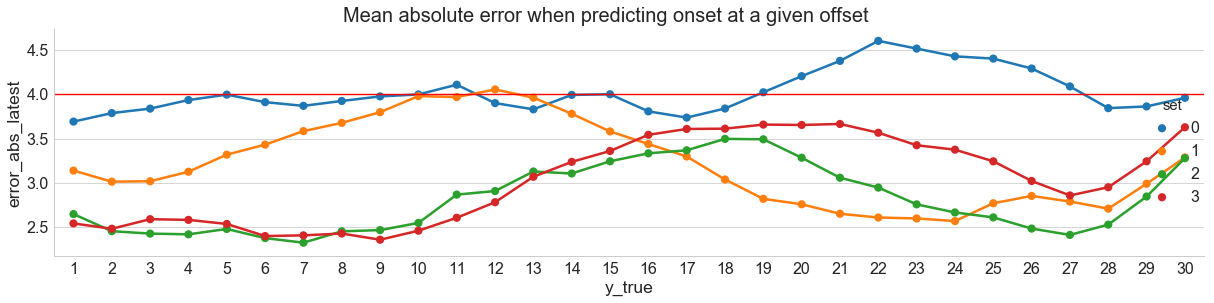
\includegraphics[width=\linewidth]{./99_appendix/img/prediction_accuracy_offset}
  \caption{The prediction accuracy of our final sets of experiments at a distance of 1-30 days from the true onset for the years in the test set (1985, 1995, 2003, 2004, 2005, 2014, 2015, 2017).}
  \label{fig:e4_prediction_accuracy_offset}
\end{figure}

\paragraph{Test accuracy for each test year}
A further interesting metric is the accuracy of the models when compared in-between years of the test set. Looking at the distributions in \cref{fig:e4_prediction_years}, we can see that there seem to be some years that are ``easier to predict'' than others. However, each set of models seems to display its best prediction skills in slightly different years. The year 2015 especially stands out, as the mean over all sets of models (even the two objectively trained ones, 0-EV12 and 4-EV06) is very similar. Further analysis of the accuracy on the test years can be found in \cref{apx:prediction_years_ci}, where we show the accuracy of each set of models subject to a 95\% confidence interval.

\begin{figure}[h!]
  \centering
  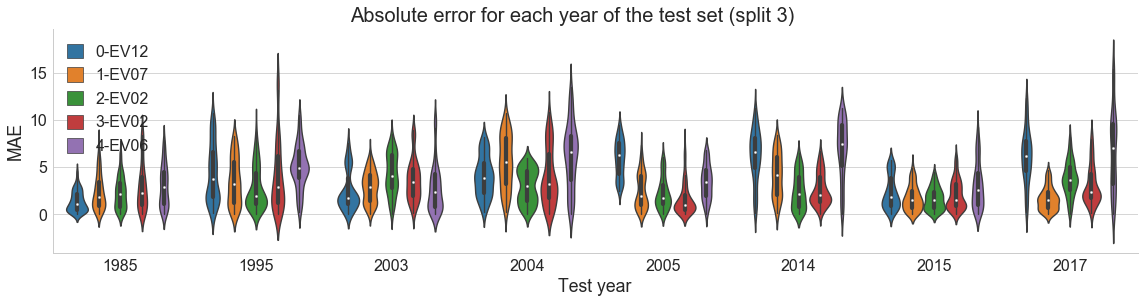
\includegraphics[width=\linewidth]{./99_appendix/img/prediction_years}
  \caption{The prediction accuracy of our final sets of experiments for the years in the test set (1985, 1995, 2003, 2004, 2005, 2014, 2015, 2017).}
  \label{fig:e4_prediction_years}
\end{figure}

\paragraph{Test accuracy with respect to the prediction date}
The results as presented in \cref{fig:e4_prediction_accuracy_offset} can be transformed in an interesting fashion: for each prediction made on the test set, we can assign the date the prediction would have been made according to the true onset date of the corresponding year. For example, given a prediction with a true distance of five days for the year 2017 (where the onset was on the 30th of May), we would end up with the 25th of May as a prediction date. Plotting these transformed results as shown in \cref{fig:e4_prediction_accuracy_dates} allows us to see how accurate we can expect a prediction to be on any given day.

\begin{figure}[h!]
  \centering
  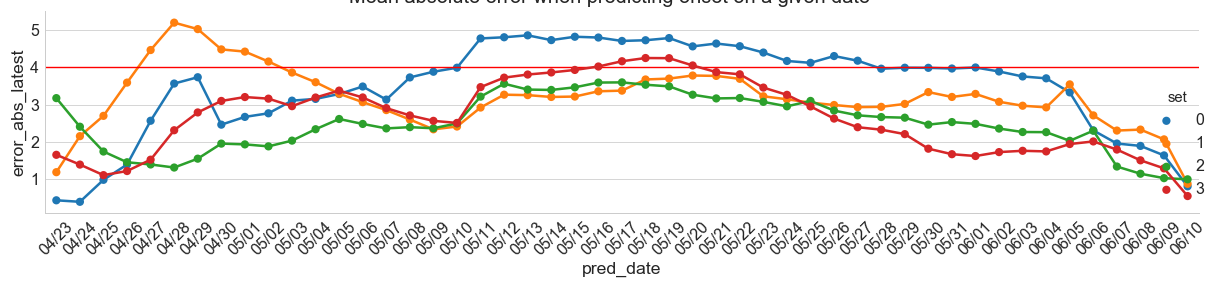
\includegraphics[width=\linewidth]{./99_appendix/img/prediction_accuracy_dates}
  \caption{The prediction accuracy of our final sets of experiments at any given date before the true onset for the years in the test set (1985, 1995, 2003, 2004, 2005, 2014, 2015, 2017).}
  \label{fig:e4_prediction_accuracy_dates}
\end{figure}

It is obviously much more useful to predict the onset earlier rather than later. According to \cref{fig:e4_prediction_accuracy_dates}, we might think that we would get our best predictions if we predicted towards the end of April. However, it has to be taken into account that not all dates in this visualization consist of the same number of predictions. The real onset dates range from dates in the second half of May to dates in mid-June, meaning that the 23d of April will only rarely be included in training or test examples. The same holds for prediction dates in early June, as they would lie after the real onset in some years. As such, predictions performed around or after the 8th of May would most certainly lead to more accurate results than predictions in April, as most training examples would include these dates. The prediction task could also be repeated every day after that, as our model is in its capabilities not restricted to only short- or long-term predictions.

\begin{figure}[h!]
  \centering
  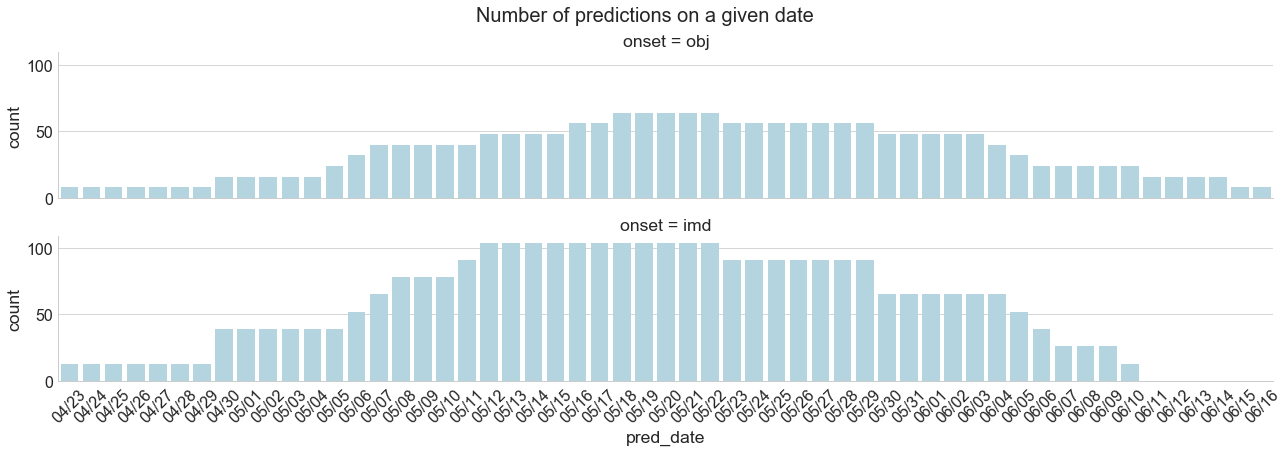
\includegraphics[width=\linewidth]{./99_appendix/img/prediction_accuracy_dates_dist}
  \caption{Number of predictions for any given prediction date for the years in the test set (1985, 1995, 2003, 2004, 2005, 2014, 2015, 2017).}
  \label{fig:e4_prediction_dist}
\end{figure}

\paragraph{Overall accuracy}
When we combine the separate measures shown previously, we get a single accuracy measure over the entire test set. As shown in \cref{tab:overall_average}, 2-EV02 is the overall most accurate model, achieving an accuracy of around 2.8 days MAE (with 2.46 days MAE as the minimum and 3.09 as the maximum over all five repetitions). The other two models that are also based on IMD onset dates (1-EV07 and 3-EV02) follow the first model closely, while the models based on objective onset dates (0-EV12 and 4-EV06) are significantly lagging behind. However, this might look different if objective onset dates were available for the entirety of the training and test years (i.e., 1979-2017).

\begin{table}[h!]
  \centering
  \begin{tabular}{rccccc}
    \toprule
    \textbf{Final evaluation set} & \textbf{0} & \textbf{1} & \textbf{2} & \textbf{3} & \textbf{4} \\
    \midrule
    \textbf{Evaluation scheme} & EV12 & EV07 & EV02 & EV02 & EV06 \\
    \textbf{Onset dates} & Objective & IMD & IMD & IMD & Objective \\
    \midrule
    \textbf{Maximum mean-absolute error} & 4.49 & 3.50 & 3.09 & 3.29 & 5.69 \\
    \textbf{Averaged mean-absolute error} & 4.11 & 3.05 & 2.82 & 3.03 & 4.25 \\
    \textbf{Minimum mean-absolute error} & 4.00 & 2.60 & 2.46 & 2.63 & 3.87 \\
    \bottomrule
  \end{tabular}
  \caption{Overall minimum, averaged and maximum mean-absolute error for the final models.}
  \label{tab:overall_average}
\end{table}

\subsection{T1-T5 and E1-E3: Other model architectures}
\label{sst:other_models}
On the path towards the well-working E4-class of models, there were many other approaches that disappointed with their learning capabilities. However, even though they did not end up to be a working model, each model architecture we have evaluated and subsequently discarded has led to important findings, without which we could not have created a working model at all. In this section, we walk through these different variations of neural network models and shortly summarize the key takeaways of each variation.

The model variations we have evaluated differ in their network structure, in the data and features used to train the models or simply in the tuning of hyperparameters applied. \cref{tab:nn_overall_summary} summarizes the key characteristics of the models we have built and evaluated and shows how the E4-class has come to be. Each model architecture is assigned a unique version identifier that we use when referring to the specific architecture (like we already did with \textit{E4}). The identifiers are based on the type of dataset used to train the model and the variation of the model architecture used (e.g., \textit{T1}: TRMM v1, \textit{E3}: ERA-Interim v3). All of the models presented were built and trained using the latest Keras 2.0 and Tensorflow 1.3/1.4 libraries for Python.

\begin{table}[h!]
  \begin{tabularx}{\linewidth}{c|X}
    \toprule
    \textbf{Model} & \textbf{Architectural Key Points} \\
    \midrule
    T1 & First trials with LSTM and TRMM; No experiments; Discarded \\
    T2 & Each location of each year as a separate example; Sequences of values for single grid cells processed with LSTM; Categorical prediction on the 11th of May (predicted MoK in 1-40 days) \\
    T3 & Each year as a separate example; One sequence of TRMM grids (daily values) per year processed with ConvLSTM2D; Numerical prediction on the 11th of May (predicted MoK in x days) \\
    T4 & Regularization for dense, convolutional and recurrent layers; Based on T3 \\
    T5 & Objective or IMD onset dates from \citet{Singh.2009}; Prediction on the 22nd of May; Based on E2 \\
    \midrule
    E1 & Training on the ERA-Interim dataset and multiple features (temperature, relative humidity); Based on T4 \\
    E2 & Objective or IMD onset dates from \citet{Singh.2009}; Prediction on the 22nd of May; Based on E1 \\
    E3 & Improved structuring of Python classes; Extraction of core model logic into base classes; Same functionality as E2; No experiments \\
    E4 & Multiple examples per year with variable offset to the onset date; Choice of additional input features; Possibility for additional 2D-convolutions before ConvLSTM2D; Switch to the functional Keras API; Based on E3 \\
    \bottomrule
  \end{tabularx}
  \caption{Overview of all neural network models that have been built \& evaluated}
  \label{tab:nn_overall_summary}
\end{table}

\subsubsection{T2: Naive classification models using TRMM}
\label{sst:nn_t2}
The first models we evaluated were classification networks based on the TRMM dataset (see \cref{st:trmm_dataset}) at various spatial resolutions (ranging from a 0.25\degree x 0.25\degree resolution to an aggregated 2.5\degree x 2.5\degree resolution).

\paragraph{Data preprocessing}
\label{ssst:nn_t2_data}
A single TRMM cell (i.e., a single location on the grid) was taken at a time and transformed into a time series for that specific location (from the first of May up to the prediction date). The latitude and longitude indices were appended in front of the time series to allow the network to learn the spatial features of each example. This led to training examples each consisting of a one-dimensional fixed-length sequence containing coordinates and daily rainfall amounts as well as a label corresponding to its category. \cref{tab:nn_t2_data} provides an overview of the structure of the examples used to train and evaluate the model.

The labels were represented as one-hot encoded vectors like $\left[ 0, ..., 1, ..., 0 \right]$. They were calculated based on the difference in days between the fixed prediction date and the monsoon onset date over Kerala. As the earliest onset in the used source \citep{Ordonez.2016} for the relevant period (1998-2017) was found to be on the 12th of May, the prediction date was set to be the 11th of May. With the latest historical onset during the available period (1887-2017) being on the 15th of June, the category labels were naturally restricted to a range of $\left[ 1, 35 \right]$. Some additional padding was added to allow for future late onsets, yielding a range of $\left[ 1, 40 \right]$. Due to the focus on the onset date over Kerala, the examples for each year could all be assigned the label for the respective year.

\begin{table}[h!]
  \centering
  \begin{tabular}{ccrrrr|c}
    \toprule
    \textbf{Latitude} & \textbf{Longitude} & \textbf{01.03.1998} & \textbf{02.03.1998} & \textbf{...} & \textbf{11.05.1998} & \textbf{Label} \\
    \midrule
    6.375 & 63.625 & 0.27 & 0.09 & ... & 3397.29 & [0, ..., 1, ..., 0] \\
    6.375 & 66.125 & 0.03 & 10.08 & ... & 4632.24 & [0, ..., 1, ..., 0] \\
    ... & ... & ... & ... & ... & ... & [0, ..., 1, ..., 0] \\
    36.375 & 91.125 & 0.79 & 0.00 & ... & 68.61 & [0, ..., 1, ..., 0] \\
    36.375 & 93.625 & 11.44 & 0.06 & ... & 40.06 & [0, ..., 1, ..., 0] \\
    \bottomrule
  \end{tabular}
  \caption{Exemplary list of training examples for the T2 architecture for the year 1998 at 2.5\degree aggregation.}
  \label{tab:nn_t2_data}
\end{table}

\paragraph{Modeling}
\label{ssst:nn_t2_model}
To build a model based on the preprocessed examples, a sequence of LSTM and Dense layers was trained on the training set. A final softmax layer allowed the prediction of classes. Losses were thereby calculated using categorical cross-entropy. A percentage of training data was randomly held out in each epoch to validate the intermediary results. \cref{lst:model_t2} shows a simplified exemplary model architecture based on the default parameters.

\begin{listing}[h!]
  \begin{minted}[linenos,
    numbersep=5pt,
    gobble=4,
    frame=lines,
    framesep=2mm]{python}

    # build a new sequential model
    model = Sequential()

    # add an LSTM layer for initial input transformation
    model.add(LSTM(128, return_sequences=False))

    # add several dense layers
    # optionally add dropout after each layer
    model.add(Dense(256, activation='relu'))
    model.add(Dense(512, activation='relu'))
    model.add(Dense(256, activation='relu'))

    # add a softmax layer for classification
    model.add(Dense(40, activation='softmax'))

    # compile the model
    model.compile(
      loss='categorical_crossentropy',
      optimizer='rmsprop',
      metrics=[top_k_categorical_accuracy])

  \end{minted}
  \caption{Simplified Python pseudocode for an exemplary T2 model (default configuration).}
  \label{lst:model_t2}
\end{listing}

\paragraph{Preliminary results}
\label{ssst:nn_t2_results}
The presented classification approach was soon discarded due to poor overall learning capabilities. Firstly, classification was found not to be a suitable approach for prediction of an upcoming onset date. An adequate loss should incorporate the numerical distance in days between the predicted and the true onset date, which is not easily possible when evaluating classification using cross-entropy loss. The implementation of a custom loss function could remediate some of these concerns but was not regarded as useful at the time.

Secondly, using each grid cell as a separate example might have led to a larger number of training examples overall, but rainfall in separate single geographical locations in India probably cannot be seen as a reasonable predictor for a large-scale phenomenon like monsoon onset. It cannot be ensured that the model would be able to learn any spatial relationships based on the inclusion of coordinates as the very first timesteps in each sequence. As we have already explored in \cref{st:ism_factors}, the behavior of Indian Summer Monsoon is influenced by many external factors that are not necessarily restricted to the Indian subcontinent. Thus it is most probably a combination of many places (some of which more important than others) that could lead to successful onset date predictions.

A further disqualifying factor against the use of any such classification approach was the fact that the model would be unable to express any future onset occurring outside the borders of the classification (e.g., more than 40 days after the prediction date). As we have elaborated in \cref{st:ism_trends}, the behavior of the ISM is ever-changing, and it cannot be ruled out that the onset date distribution will change significantly in the time to come.

\subsubsection{T3 \& T4: First convolutional models using TRMM}
\label{sst:nn_t3}
The findings of the first naive classification suggested that the overall model architecture and the data input shape needed to be rethought. To be able to capture temporal as well as spatial relationships between different geographical locations in India, the input time series needed to be changed such that each timestep would contain daily data for the entire Indian subcontinent.

\paragraph{Data preprocessing}
\label{ssst:nn_t3_data}
To extend the dimensionality of the input data, the TRMM dataset was transformed to a fixed-length sequence of coordinate grids (each coordinate grid thereof containing data for all locations). This resulted in only a single training example per year of data. As TRMM data is available from 1998 onwards and with some data that would be held out for validation and testing, the number of training examples shrunk to roughly a dozen.

Furthermore, keeping the outcome calculations the same as for the previous classification task, the classification was changed to numerical regression. Instead of trying to predict one of the classes in the range $\left[ 1, 40 \right]$, the model would thus predict an exact number that could be both higher or lower than numbers in the classification range. However, the prediction would still represent the predicted number of days from the prediction date until the occurrence of monsoon onset over Kerala.

\begin{table}[h!]
  \centering
  \begin{tabular}{rrrrrr}
    \toprule
    \textbf{Lat./Lon.} & \textbf{63.375} & \textbf{64.375} & \textbf{...} & \textbf{95.375} & \textbf{96.375} \\
    \midrule
    6.125 & 849.779974 & 791.189987 & ... & 139.547018 & 430.566095 \\
    7.125 & 323.249996 & 393.899986 & ... & 38.789999 & 172.289993 \\
    ... & ... & ... & ... & ... & ...\\
    38.125 & 0.000000 & 0.000000 & ... & 1.648755 & 7.281448 \\
    39.125 & 0.000000 & 0.000000 & ... & 1.584739 & 1.154755 \\
    \bottomrule
  \end{tabular}
  \caption{An exemplary coordinate grid aggregated to 1.0\degree. A sequence of 72 such matrices and its label correspond to a full training example for the T3/T4 models (one year of data).}
  \label{tab:nn_t3_data}
\end{table}

\paragraph{Modeling}
\label{ssst:nn_t3_model}
To be able to process a sequence of grids (i.e., matrices), the first layers of the model needed to be able to handle multi-dimensional input sequences. Said layers were therefore changed from a regular LSTM layer to Convolutional LSTM layers (see \cref{sst:neural_networks} on ConvLSTM2D layers). These layers can process a sequence of multi-dimensional input matrices and learn complex spatial as well as temporal relationships.

The new model architecture (T3) further included batch normalization to improve training speed. Furthermore, in comparison to the previously used cross-entropy loss, mean-squared or mean-absolute error could now provide a reasonable distance metric. \cref{lst:model_t3} shows an exemplary model configuration using default parameters.

A later extension (T4) added regularization for the convolutional, recurrent and dense layers to improve the models' ability to generalize. Furthermore, the validation set was changed from a random percentage of the training set to a fixed set of years. The validation years were defined to be the latest in the training set such that long-term trends could be captured by the model, which might not have been possible using the previous random validation split.

\begin{listing}[h!]
  \begin{minted}[linenos,
    numbersep=5pt,
    gobble=4,
    frame=lines,
    framesep=2mm]{python}

    # start building a sequential model
    model = Sequential()

    # add a first convolutional LSTM layer
    model.add(ConvLSTM2D(filters=32, kernel_size=(7, 7), activation='relu'))
    model.add(BatchNormalization())
    model.add(Dropout(0.4))

    # add a second convolutional LSTM layer
    model.add(ConvLSTM2D(filters=16, kernel_size=(5, 5), activation='relu'))
    model.add(BatchNormalization())
    model.add(Dropout(0.4))

    # add a third convolutional LSTM layer
    model.add(ConvLSTM2D(filters=8, kernel_size=(3, 3), activation='relu'))
    model.add(BatchNormalization())
    model.add(Dropout(0.4))

    # add max pooling before flattening to reduce the dimensionality
    model.add(MaxPooling2D(pool_size=(4, 4))

    # flatten to make data digestible for dense layers
    model.add(Flatten())
    model.add(BatchNormalization())

    # first dense layer
    model.add(Dense(1024, activation='relu'))
    model.add(BatchNormalization())
    model.add(Dropout(0.6))

    # second dense layer
    model.add(Dense(512, activation='relu'))
    model.add(BatchNormalization())
    model.add(Dropout(0.6))

    # third dense layer
    model.add(Dense(256, activation='relu'))
    model.add(BatchNormalization())
    model.add(Dropout(0.6))

    # single linear neuron for numerical prediction
    model.add(Dense(1))

    # compile the model
    model.compile(
      loss='mean_squared_error',
      optimizer='rmsprop',
      metrics=['mean_squared_error', 'mean_absolute_error'])

  \end{minted}
  \caption{Simplified Python pseudocode for an exemplary T3 model (default configuration).}
  \label{lst:model_t3}
\end{listing}

\paragraph{Preliminary results}
\label{ssst:nn_t3_results}
Many experiments with various hyperparameter tunings showed that the first variation of the model architecture (T3) was unable to fully learn the concepts of the training set and that it did not generalize to the validation set very well.

The results of experiments for the T4 variation were much improved, especially if regularization was used for all types of layers (in addition to dropout). In training, the model converged up to a certain point but tended to plateau afterward, even if run for hundreds of epochs. This would normally suggest that the optimization process has reached either a minimum or is otherwise unable to learn any further, except that in this case, the validation loss plateaued as well (instead of increasing due to a growing tendency to overfit).

\begin{figure}[h!]
  \centering
  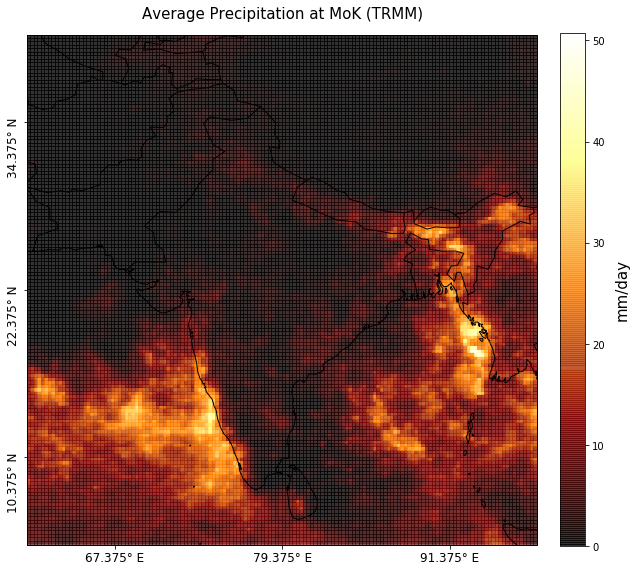
\includegraphics[width=0.5\linewidth]{./99_appendix/img/prec_avg_onset}
  \caption{Average precipitation at monsoon onset over Kerala (TRMM, 1998-2017)}
  \label{fig:trmm_prec_onset}
\end{figure}

We found that, in this case, the models learned a way to get close to the real outcomes without learning anything particularly useful about the patterns in the input data: all the outcomes of the validation and test sets were simply predicted to be the mean value of the outcomes in the training set. There could be several explanations for this behavior, of which most suggest that something is off with the input data. It might be that the sparsity of the TRMM dataset (as visualized in \cref{fig:trmm_prec_onset}) and its many places without any rainfall prevent the neural network from learning any useful patterns. Alternatively, it could be that we are trying to find patterns in the input data that don't exist in the way we would have imagined (i.e., that we are trying to fit a model to noise).

\subsubsection{E1: Convolutional models using ERA-Interim}
\label{sst:nn_e1}
The overall results from T1 up to T4 suggested that the TRMM dataset on its own might not be well suited for the prediction task at hand. An obvious way of improvement was to use another dataset for the prediction tasks, namely the ERA-Interim reanalysis dataset.

Compared to the TRMM dataset, the ERA-Interim dataset brings with it several advantages relevant to our task. Firstly, much more data is available (dating back to 1979 instead of 1998), which can improve the performance of deep neural networks significantly (even though the number of total examples is still comparatively small). Secondly, there are many more features (of which some could prove to be better predictors than solely the amount of daily rainfall). Furthermore, the dataset had already been used for onset prediction tasks in \citep{Stolbova.2015}.

A disadvantage of using the ERA-Interim dataset might be that its spatial resolution is much lower than the one of the TRMM dataset (0.75\degree x 0.75\degree compared to 0.25\degree x 0.25\degree). When training with the ERA-Interim dataset, the input matrices in the sequence would thus be much smaller in the spatial dimensions (latitude and longitude), providing the models with less detailed data to train on. However, many more ERA-Interim features could be added as channels to the model inputs, giving the models the possibility to learn more complex patterns and relationships. The lower resolution of the ERA-Interim dataset further means that each input matrix is up to 9 times smaller than with TRMM, leading to lower overall computational effort and hardware requirements (i.e., memory capacity).

\paragraph{Data preprocessing}
\label{ssst:nn_e1_data}
This first iteration of the ERA-based model (E1) made use of only two features from ERA-Interim: temperature and relative humidity each at a 1000hPa pressure level. \citet{Stolbova.2015} found this combination of features to be a reliable predictor of the monsoon onset date. While this finding should also apply to our problem, the approach used was based on statistical time-series analysis and prediction and as such might not directly transfer to the training of our neural network models.

To feed temperature and relative humidity to the model simultaneously, the features needed to be stacked in a single coordinate grid. Each grid cell would thus contain multiple channels (i.e., features, same as the RGB channels in images) and be represented as a 3D-tensor (i.e., a "3D matrix"). Combining grids to a sequence yielded a sequence of 3D-tensors (a 4D-tensor) that could then be used as input for the neural network models.

\paragraph{Modeling}
\label{ssst:nn_e1_modeling}
Incorporating these findings into a new model structure, we extended the convolutional and regularized T4 model to be able to learn from a sequence of 3D-tensors. The convolutional layers would then process these inputs just like they would process an RGB image with its three channels. The architecture for this is shown in \cref{lst:model_e1}.

\begin{listing}[h!]
  \begin{minted}[linenos,
    numbersep=5pt,
    gobble=4,
    frame=lines,
    framesep=2mm]{python}

    # start building a sequential model
    model = Sequential()

    # add a ConvLSTM2D layer
    model.add(
      ConvLSTM2D(
        filters=16,
        kernel_size=(7, 7),
        activation='tanh',
        recurrent_activation='hard_sigmoid',
        kernel_regularizer=regularizers.l2(0.02),
        recurrent_regularizer=regularizers.l2(0.02)))

    model.add(MaxPooling3D(pool_size=(1, 2, 2)))
    model.add(BatchNormalization())
    model.add(Dropout(0.6))

    # ... repeat with 5x5/8 and 3x3/4

    # flatten to make data digestible for dense layers
    model.add(Flatten())
    model.add(BatchNormalization())

    # add a new dense layer
    model.add(Dense(1024, activation='relu', kernel_regularizer=regularizers.l2(0.02)))
    model.add(BatchNormalization())
    model.add(Dropout(0.6))

    # ... repeat with 512 and 256 nodes

    # final dense layer for numerical prediction
    model.add(Dense(1))

    # compile the model
    model.compile(
      loss='mean_squared_error',
      optimizer=RMSprop(lr=0.01),
      metrics=['mean_squared_error', 'mean_absolute_error'])

  \end{minted}
  \caption{Simplified Python pseudocode for an exemplary E1 model (default configuration).}
  \label{lst:model_e1}
\end{listing}

\paragraph{Preliminary results}
\label{ssst:nn_e1_results}
Running experiments for the E1 model yielded results that displayed similar patterns to the TRMM-based models evaluated before: the models were learning up to a certain point and plateaued at unsatisfactory levels of loss and validation loss. They still seemed to get stuck during the learning process.

As experiments for entirely different datasets (TRMM and ERA) and many hyperparameter tunings for each showed similarly unsatisfactory patterns, it was probable that something was off with the data being fed into the model. Further research showed that the distribution of onset dates used seemed to show some irregularities that had not been regarded as irregular before: many onset dates were set in the first half of May (as early as on the 12th of May), which is highly improbable for typical ISM onsets\footnote{This was brought to light during consultation with V. Stolbova.}. These onset dates might, for example, have been caused by bogus monsoon onsets that were not registered as such at the time.

The labels of the training, validation and test examples were all calculated using the skewed onset dataset. The early outliers in the dataset forced us to predict even earlier, which is why predictions up to this point were always made on the 11th of May, and why the sequences were restricted to the 72 days in between 01.03-11.05 of each year.

\subsubsection{E2, E3 \& T5: Convolutional models with objective onset dates}
\label{sst:nn_e2t5}
After further analysis of onset distributions for different onset datasets, the objective definition of monsoon onset proposed by \citet{Singh.2009} seemed to be the most adequate for our training at the time. The distribution seemed to be much less skewed overall, with more similarities to a uniform distribution than to a Gaussian normal distribution, at least when data was restricted to the relevant area between 1979-2017 (see \cref{apx:onset_dates} for the full analysis). Notice that we found out only during the final evaluation of the E4 models that the IMD onsets calculated by \citet{Singh.2009} work even better, especially as they need to be combined with official IMD dates after 2007 (yielding one ``single'' distribution).

While it might be counterintuitive that the ISM onset would not follow a normal distribution (as many natural processes do), a more balanced distribution of labels can improve the performance of machine learning models. Many models work better if input data is preprocessed with stratification methods (i.e., classes are rebalanced), as the model might otherwise tend to predict the label that occurs most often in the training set.

Building on these findings, we then created the E2, E3 and T5 model versions, i.e., new models for both ERA-Interim and TRMM (as well as a combination of them) that were primarily a repetition of the best previous experiments with updated labels for the new onset dates.

\paragraph{Data preprocessing}
\label{ssst:nn_e2t5_data}
Due to the new distribution of onset dates, the prediction date was newly set on the 22nd of May, increasing the available sequence length by 11 days (up to 83 days). The preprocessing otherwise didn't change much, as the TRMM dataset could simply be regarded as a one-channel version of the stacked ERA-Interim features.

\paragraph{Modeling}
\label{ssst:nn_e2t5_modeling}
The models were not much changed either, as they were already flexible enough to accept arbitrary sequence lengths and an arbitrary number of stacked features (channels). The main changes were mostly refactorings and optimizations in the order of layers. As such, we do not explicitly show the source for these kinds of models.

\paragraph{Preliminary results}
\label{ssst:nn_e2t5_results}
Running the experiments for E2 and T5 yielded much better final losses. The validation loss could get as close as 2.5 days (TRMM) and 4.7 days (ERA) of mean-absolute error, which would suggest that T5 could predict the monsoon onset on the 22nd of May and do so with an accuracy of +- 2.5 days, which would have been a good result.

However, close examination of the actual predictions of the model was not as reassuring, as the model still seemed to predict only one single number for any validation or test example that was fed into the model. Furthermore, a combination of the TRMM and ERA dataset by stacking the three features yielded comparable results: the model again seemed to resort to predicting the mean of onsets based on the TRMM dataset. Additionally, stacking the TRMM and the ERA-Interim dataset necessitated that we excluded years before 1998 from the ERA-Interim dataset, causing a hefty loss of available training data.

\subsubsection{The development of the E4-models}
\label{sst:nn_e4}
Following the bad generalization capabilities of all models up to their latest versions, an improvement to the overall training approach was sought. Up to versions E3 and T5, the dates of prediction were always fixed to a single date during the pre-monsoon period (22nd of May). This meant that for each year of data, only a single sequence could be extracted and used as a training example.

The patterns during the pre-monsoon period might not be conclusive enough to allow a model to predict future onsets reliably. Some patterns might be closely tied to a temporal distance to the monsoon onset, i.e., some event might always happen approximately two weeks before onset. This would have been captured by the model at different steps in the sequence, which could, in turn, have been suitable for prediction. On the other hand, the model might have missed many of these events because the data was cut off at a fixed prediction date, possibly multiple weeks before the real onset date.

To allow a model to capture all the events leading up to the onset of each respective year, the approach to training the model thus needed to be changed. Firstly, the model needed to be fed sequences with equal distances to the respective real onset date. For example, with an onset on the 10th of June, the sequence to be fed to the model could include data from the 9th of May to the 9th of June. Repeating this for each year in the training set while keeping a one-day distance to the real onset date and the length of the sequences fixed, the model should learn to predict that the onset will take place in exactly one day.

This would not be that useful by itself, as the model would then only be able to predict the onset one day in advance. However, this approach to training allows feeding the model multiple sequences per year, each with a different offset to the onset date and a correspondingly different label. The amount of available examples is as such greatly increased: generating three such sequences per year would triple the overall number of examples available for training. Furthermore, the prediction capabilities of the model could then be evaluated separately for each offset, yielding results on how well the model can predict one day in advance, one week in advance or even multiple weeks in advance.

The detailed architecture and evaluation of this final model architecture have already been described in depth in previous sections (\cref{sst:final_model}, especially). Having described all the models that we used during the creation of this work, we now conclude this chapter in the next section, and our work in the section after that.

\section{Conclusion}
In this second part of our work, we have described the different approaches to monsoon onset prediction that we have evaluated, along with their results. Next to many experiments that we would consider failures based simply on their prediction results, we have found a model architecture that can learn from the ERA-Interim dataset and accurately predicts the ISM onset from up to a one month lead. The architecture is based on the ConvLSTM network layers we have introduced early on and combines several of these layers with a sequence of fully-connected layers for further learning. A prediction is finally performed by a single-neuron output layer with linear activation.

While we have evaluated models based on different datasets for both input features and monsoon onset dates, we have found the ERA-Interim dataset to work best, especially when used in combination with IMD onset dates from \citet{Singh.2009} and the IMD. The TRMM dataset was also evaluated but led to models that were unable to learn any useful patterns, which might have been caused by the natural sparsity of precipitation.

The accuracy achieved by our final model outperforms comparable methods like the official IMD prediction model (four days RMSE) or the approach presented in \citet{Stolbova.2015} with an accuracy of $\pm$ seven days. Over repeated evaluation of our overall best-performing model, the maximum mean absolute error of a repetition was 3.09 days, while the minimum was 2.46 days and the mean absolute error over all repetitions was 2.82 days.


\chapter{Conclusion}
\label{c:conclusion}
The Indian Summer Monsoon is one of the most influential meteorological phenomena on earth. Even though the ISM occurs every year, the exact timing and strength of its occurrence are subject to great variability and a primary factor for the welfare of the population in countries all over the Indian subcontinent. In a first part of this work, we have sought to provide insight into the strength of monsoon rainfalls by analyzing the spatial distribution of extreme rainfall events. The second part was then dedicated to the problem of predicting the timing of ISM onset over Kerala. With both of these parts, we have tried to reduce the uncertainty that is caused by the variability of ISM behavior. This chapter serves as a final conclusion to our work, with the main findings and results summarized in \cref{st:conclusion_summary} and possible extensions of our work described in \cref{st:conclusion_outlook}.

\section{Summary \& Final Conclusions}
\label{st:conclusion_summary}
Trying to provide more insight into the strength of the ISM, we have analyzed extreme monsoon rainfall using event synchronization methods and produced climate networks representing the spatial distribution of extreme rainfall events. We have then analyzed these climate networks with network measures like degree, betweenness centrality and PageRank, resulting in an intuition about the importance of locations concerning extreme rainfall. When compared to the foundational work of \citet{Stolbova.2015}, we have identified similar key regions for the pre-monsoon and monsoon seasons: while the Indian Ocean and the Tibetan Plateau are the most influential regions before the onset of the ISM, North Pakistan dominates the climate networks during the monsoon season. Our results for the post-monsoon season differ from the results in the foundational work, as the important locations in our network are concentrated over central India and the Tibetan Plateau, while the results from \citet{Stolbova.2015} primarily focus on the Tibetan Plateau.

For all of our climate network results, we have tried to link the previously described patterns to well-known phenomena that drive the yearly development of the ISM. The pre-monsoon season corresponds to the Indian summer, in which the country regularly experiences temperatures of more than 40\degree Celsius. Additionally, most rainfall is concentrated over the oceans in this season. The monsoon season is characterized by a reversal of the land-ocean temperature gradient, leading to a sea-breeze that brings moisture from the oceans onto the land. While it is non-trivial to interpret a distinct pattern like the one over North Pakistan, we proposed that the region could serve as a pivot between other key regions during this season. The final monsoon season we have analyzed, the post-monsoon season, is the season where the ISM fully withdraws from the subcontinent, and the following north-east monsoon starts to build up. We have proposed that this might cause patterns like the one seen over central India and the Tibetan Plateau.

While our first results were based mostly on the work of \citet{Stolbova.2015}, we have extended her climate network analysis by the PageRank measure as well as weighted and directed climate networks and networks thresholded at different percentiles. The PageRank of directed networks shows some new patterns when compared to the degree, as the intuition of importance is different in its ranking procedure. Further, we have found that a weighting of network edges with their synchronization coefficient makes little difference in the overall patterns and only changes minimal details. While the results of \citet{Stolbova.2015} are based on the TRMM dataset at its full resolution (0.25\degree), we have reduced the dimensionality and thus the computational requirements of the dataset by aggregating the resolution to 0.75\degree. While this could also be a reason for some of the differences in our results, they largely seem to match for two out of three seasons, with only the third season displaying bigger differences.

The second main research question in this work was the prediction of ISM onset, for which we have built prediction models based on recent neural network methods. After a long process of parameter tuning and model building, we finally got to a model architecture that manages to predict ISM onset better than comparable methods and does so from up to a one month lead. Official IMD predictions achieve a root-mean-squared error of around four days, meaning that the monsoon onset prediction can be interpreted as accurate if the real onset occurs up to four days earlier or later than the predicted date. \citet{Stolbova.2015} even counts predictions as accurate if the real onset is up to seven days early or late. In comparison, repeated evaluation of our best model yields an overall mean absolute error of 2.82 days when predicting between one and thirty days before the monsoon onset. The mentioned model tends to predict best during the week leading up to the monsoon onset, as well as more than three weeks before the onset, but performance is still good in between these periods.

Our overall best-performing model architecture takes several features of the ERA-Interim reanalysis dataset as input (mean sea-level pressure, temperature and relative humidity). Based on these inputs, a sequence of ConvLSTM and fully-connected layers manages to perform an accurate numerical prediction. On any day during the month leading up to the ISM onset, we can use our model to predict the number of days that remain until the monsoon arrives. Predictions could even be performed every day, resulting in updated predictions as more data gets available.

Even though the predictions are quite accurate, an important shortcoming in this model architecture is the practicality of the prediction approach. We trained the majority of our neural network models based on the ERA-Interim dataset, which is a meteorological reanalysis computed from both observations and simulations. The data assimilation and quality control procedures of such reanalysis datasets take their time, which is why the ERA-Interim dataset is only published with a two-month delay (not in real-time). This means that the ERA-Interim dataset cannot practically be used to predict the ISM onset, as the data for the full pre-monsoon season is only released in July. However, our architecture still can still serve as a proof that onset prediction can be performed by applying neural networks to spatiotemporal meteorological datasets and could further be used as a foundation for future models.

\newpage
\section{Future Work}
\label{st:conclusion_outlook}
The work we have presented so far could be extended in several ways, of which some would require more effort than others. In this final part of our work, we introduce the possible future extensions we could imagine and state some of our ideas for their implementation.

\paragraph{Prediction of extreme rainfall events}
The analysis of climate networks as shown in this work is only a starting point, after which a next logical step could be the prediction of extreme rainfall events. For example, one could try to predict future extreme events at a location basing on extreme events in strongly synchronous locations (that tend to lead said location).  This approach could probably only be used for short-term prediction, as the lead-time of synchronous events tends to lie within only a few days. However, even short-term predictions could potentially make a big difference concerning the safety of people affected by the predicted event.

\paragraph{Usage of different datasets}
Our final prediction model is fully focused on the ERA-Interim dataset and several of its features. While the predictions based thereon seem to be accurate and manage to outperform other comparable models, the practicality of a model based on such a reanalysis dataset is not as high as one would wish. Reanalysis datasets like ERA-Interim are only released after a certain delay (i.e., two months for ERA-Interim), which is needed for the producers to be able to perform data assimilation and quality control procedures. However, this also means that most pre-monsoon data is only fully available once the monsoon has most certainly already arrived. We suggest that the models we proposed could serve as a foundation for models that directly base on real-time datasets or purely observational datasets, and possibly multiple of them.

\paragraph{Usage of climate network results for onset prediction}
As of now, the two parts of this work, the evaluation of climate networks and the prediction of ISM onset, are strictly separate. However, a combination of the two could be imaginable, where a network measure like PageRank could be used as an additional input feature for neural network models. Such an additional feature might provide weights for the locations on the grid, which could help a neural network identify ``important'' locations that might work well as a predictor of monsoon onset.

\paragraph{Dense prediction}
Our work is solely focused on the prediction of the monsoon onset over Kerala, as it marks the arrival of monsoon on the Indian subcontinent. However, as we have described early on, an accurate estimate of monsoon arrival is of high importance for people all over India. Therefore, it would be much more useful if accurate predictions were available for all regions of India.

As a future improvement of the general applicability of our neural network models, we suggest the evaluation of an approach using ``dense prediction'' methods. Dense prediction models predict a label for each unit of the input, where a unit could be a single pixel or a region of the input image. A similar approach has been successfully applied to problems like video frame prediction, where, based on the past few frames, the next frame is to be predicted. The original work describing the ConvLSTM neural network architecture has in a sense also performed a dense prediction task, as future radar maps have been predicted based on past radar maps.

When applied to the problem of monsoon onset prediction, we could imagine that a future model would be trained to predict matrices containing the days until ISM onset for different patches of the Indian subcontinent. As we have successfully used the IMD onset dates as extracted from \citet{Singh.2009}, we would suggest a matrix with predictions based on the subregions described therein (as shown in \cref{fig:singh_subregions}). A suitable approach for handling patches of the input that are not part of any of the subregions would still need to be found, as the output dimensions of dense prediction tasks are typically equal to the input dimensions.

\begin{figure}[h!]
  \centering
  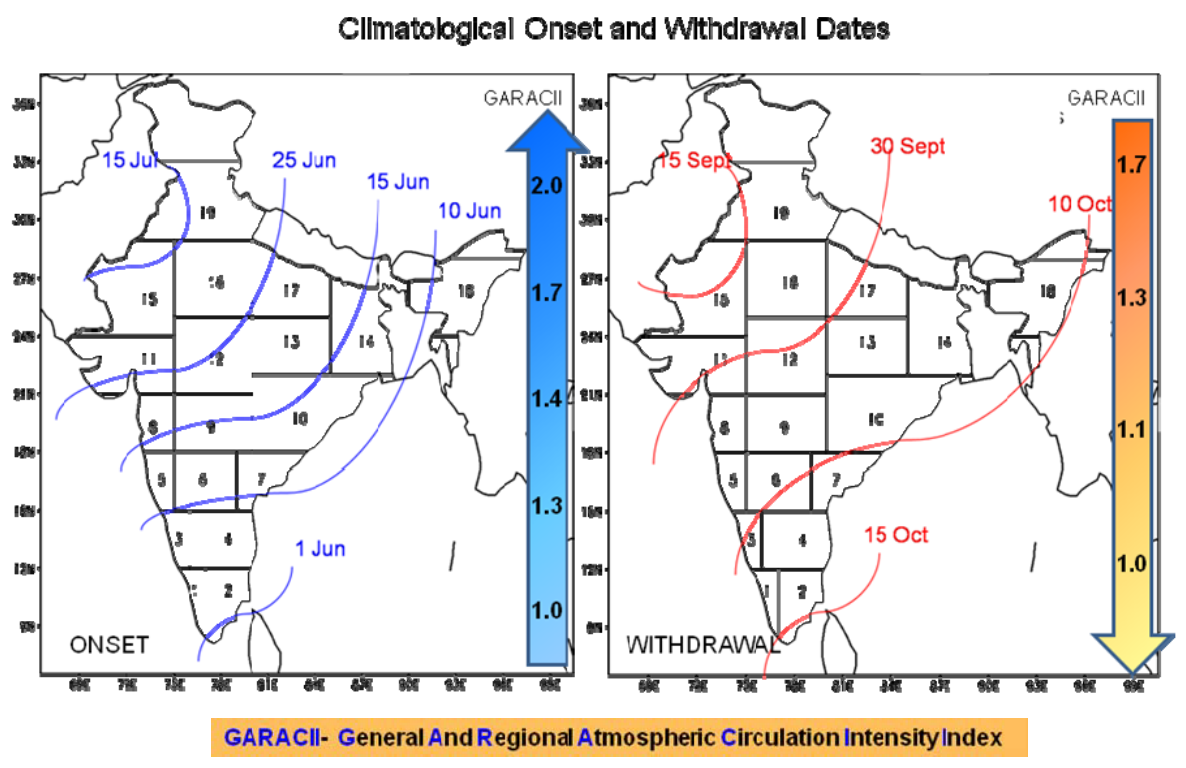
\includegraphics[width=0.6\textwidth]{./99_appendix/img/singh_subregions.png}
  \caption{Regular monsoon onset and withdrawal dates for the 19 subregions of the Indian subcontinent as depicted in \citet{Singh.2009}.}
  \label{fig:singh_subregions}
\end{figure}

\paragraph{Prediction of monsoon withdrawal}
While we have focused on predicting the monsoon onset, the withdrawal of monsoon is of similarly high importance to the Indian population, as it marks the transition from the rainy season to the winter months. Basing on our final model architecture, the withdrawal dates of the ISM could be predicted without necessitating any large changes. Using data for the monsoon season as extracted from ERA-Interim and onset dates from the IMD and \citet{Singh.2009}, a well-tuned model should be able to predict monsoon withdrawal with reasonable accuracy.


% *************** Bibliography ***************
\bibliographystyle{apalike}
\bibliography{99_references/thesisbib}

% *************** Appendixes ***************
\appendix
\chapter{Appendix}
\label{apx:appendix}

\clearpage
\section{Monsoon Onset Dates}
\label{apx:onset_dates}

\begin{figure}[h]
  \centering
  \begin{tabular}{cc}
    \subfloat{
      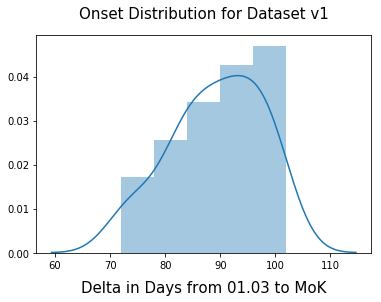
\includegraphics[width = 0.35\linewidth]{./99_appendix/img/onset_hist_v1}} &
    \subfloat{
      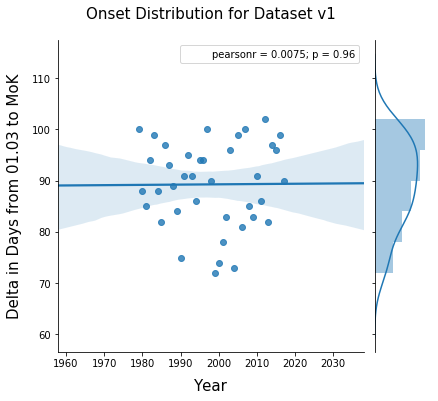
\includegraphics[width = 0.4\linewidth]{./99_appendix/img/onset_joint_v1}} \\
    \subfloat{
      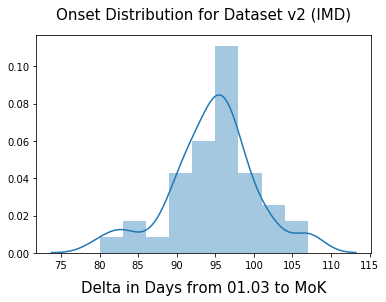
\includegraphics[width = 0.35\linewidth]{./99_appendix/img/onset_hist_v2_imd}} &
    \subfloat{
      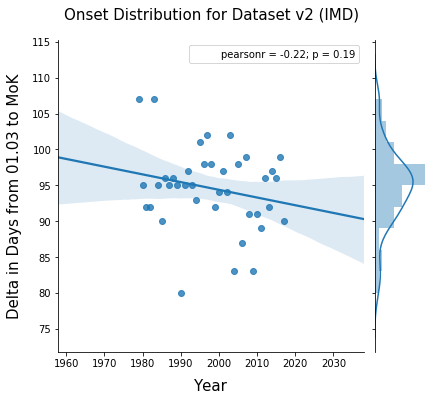
\includegraphics[width = 0.4\linewidth]{./99_appendix/img/onset_joint_v2_imd}} \\
    \subfloat{
      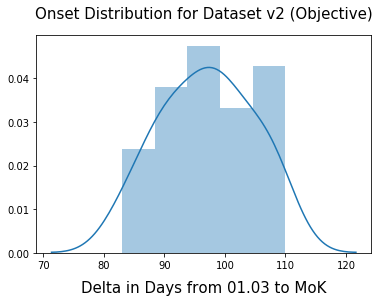
\includegraphics[width = 0.35\linewidth]{./99_appendix/img/onset_hist_v2_obj}} &
    \subfloat{
      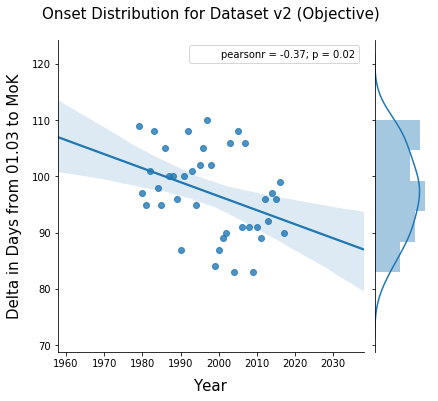
\includegraphics[width = 0.4\linewidth]{./99_appendix/img/onset_joint_v2_obj}} \\
  \end{tabular}
  \caption{Overview of Onset Distributions (1979-2017, v1: \citet{Ordonez.2016, IndiaMeteorologicalDepartment.2017b}, v2: \citet{Singh.2009, IndiaMeteorologicalDepartment.2017b}}
  \label{apx:onset_distributions}
\end{figure}

\begin{figure}[h]
  \centering
  \begin{tabular}{cc}
    \subfloat{
      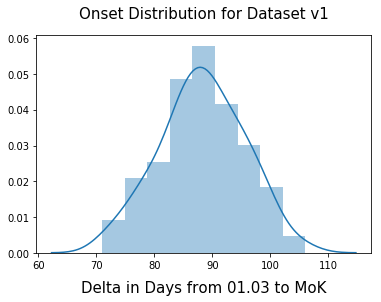
\includegraphics[width = 0.35\linewidth]{./99_appendix/img/onset_hist_v1_uncut}} &
    \subfloat{
      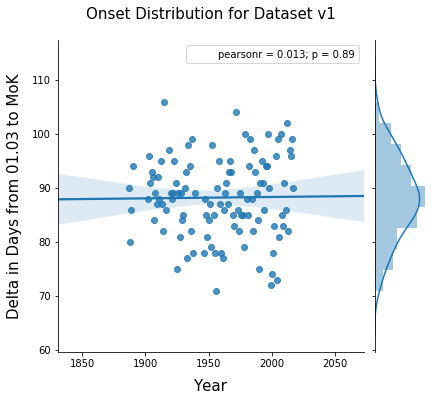
\includegraphics[width = 0.4\linewidth]{./99_appendix/img/onset_joint_v1_uncut}} \\
    \subfloat{
      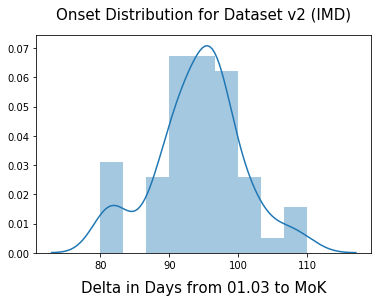
\includegraphics[width = 0.35\linewidth]{./99_appendix/img/onset_hist_v2_imd_uncut}} &
    \subfloat{
      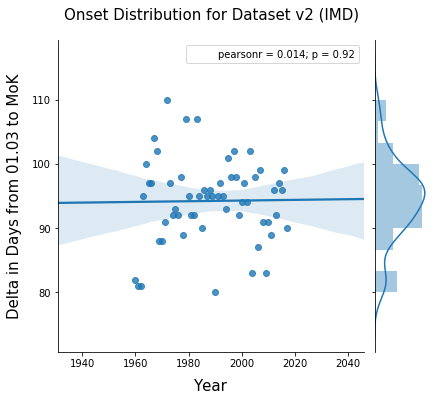
\includegraphics[width = 0.4\linewidth]{./99_appendix/img/onset_joint_v2_imd_uncut}} \\
    \subfloat{
      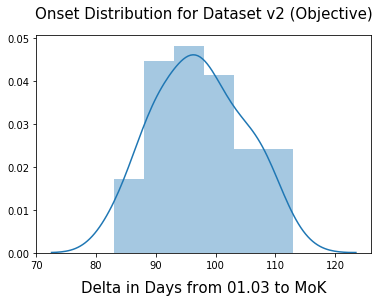
\includegraphics[width = 0.35\linewidth]{./99_appendix/img/onset_hist_v2_obj_uncut}} &
    \subfloat{
      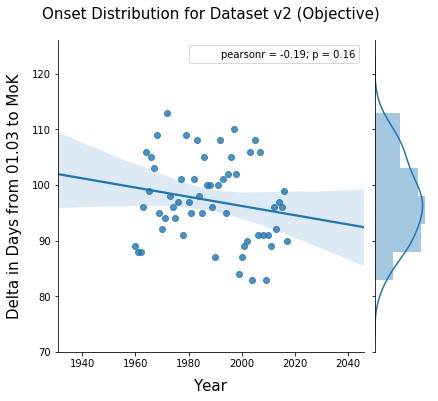
\includegraphics[width = 0.4\linewidth]{./99_appendix/img/onset_joint_v2_obj_uncut}} \\
  \end{tabular}
  \caption{Overview of Onset Distributions (v1: 1887-2017, \citet{Ordonez.2016, IndiaMeteorologicalDepartment.2017b}, v2: 1960-2017, \citet{Singh.2009, IndiaMeteorologicalDepartment.2017b})}
  \label{apx:onset_distributions_uncut}
\end{figure}

\clearpage
\section{TRMM \& ERA}
\label{apx:trmm_era}

\subsection{Getting the Datasets}
\label{apx:download}
\begin{itemize}
  \item TODO: Subsetting and Downloading (with Giovanni etc.)
\end{itemize}

\subsection{Usage with Python}
\begin{itemize}
  \item TODO: NetCDF4 vs. GRIB
  \item TODO: Python Libraries for handling NetCDF4
  \item TODO: Pseudocode for import
\end{itemize}

\clearpage
\subsection{Feature Analysis}

The visualizations in this section show the development of different ERA and TRMM features over the duration of an average monsoon. To calculate the visualizations, the data for each feature has been averaged over all years of available data (1998-2017 for TRMM, 1979-2017 for ERA).

\textbf{Example:} The temperature grids 10 days previous to the objective onset dates (Monsoon over Kerala, MoK; \ref{apx:era_t}) for all available years are extracted and then averaged to yield an averaged grid representation. The visualization is then simply calculated based on the averaged grid.

\begin{figure}[h]
  \centering
  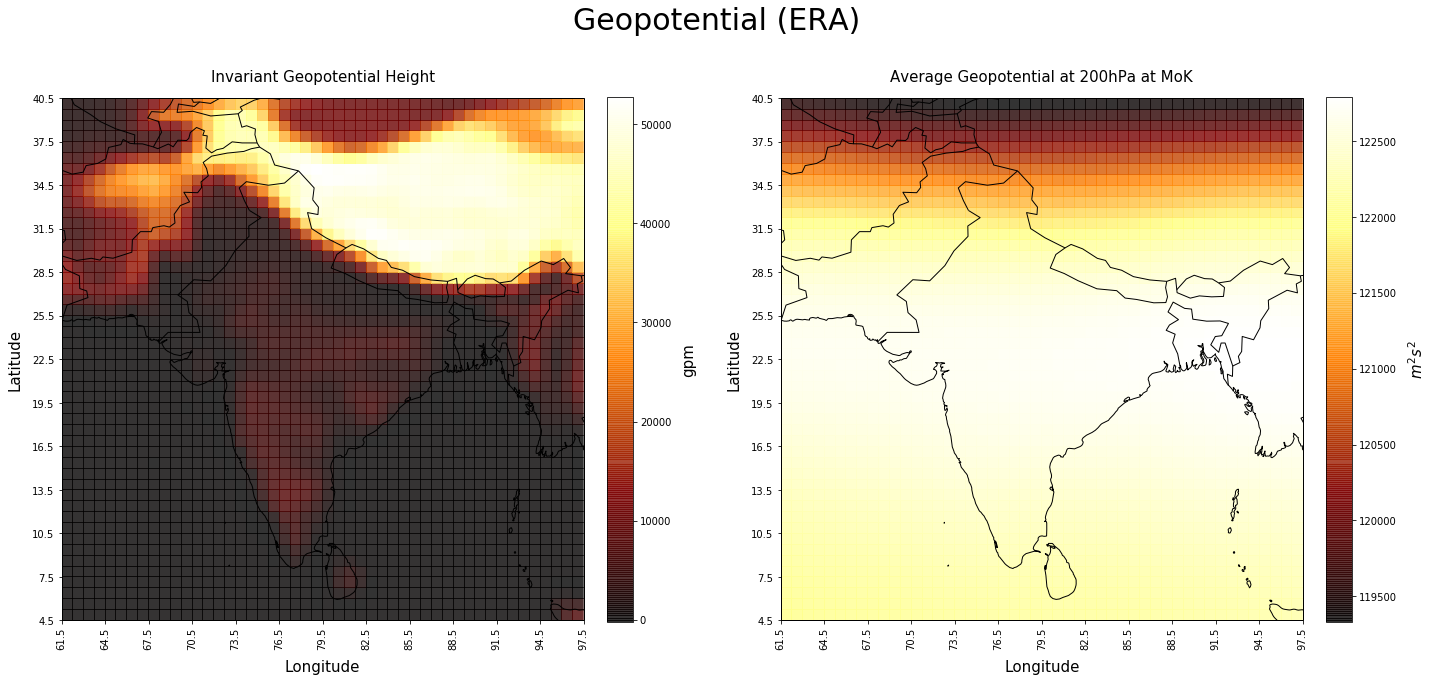
\includegraphics[width=\linewidth]{./99_appendix/img/geopotential}
  \caption{Geopotential Height and Geopotential at 200hPa (ERA-Interim, 1979-2017)}
  \label{apx:era_geopotential}
\end{figure}

\begin{figure}[h]
  \centering
  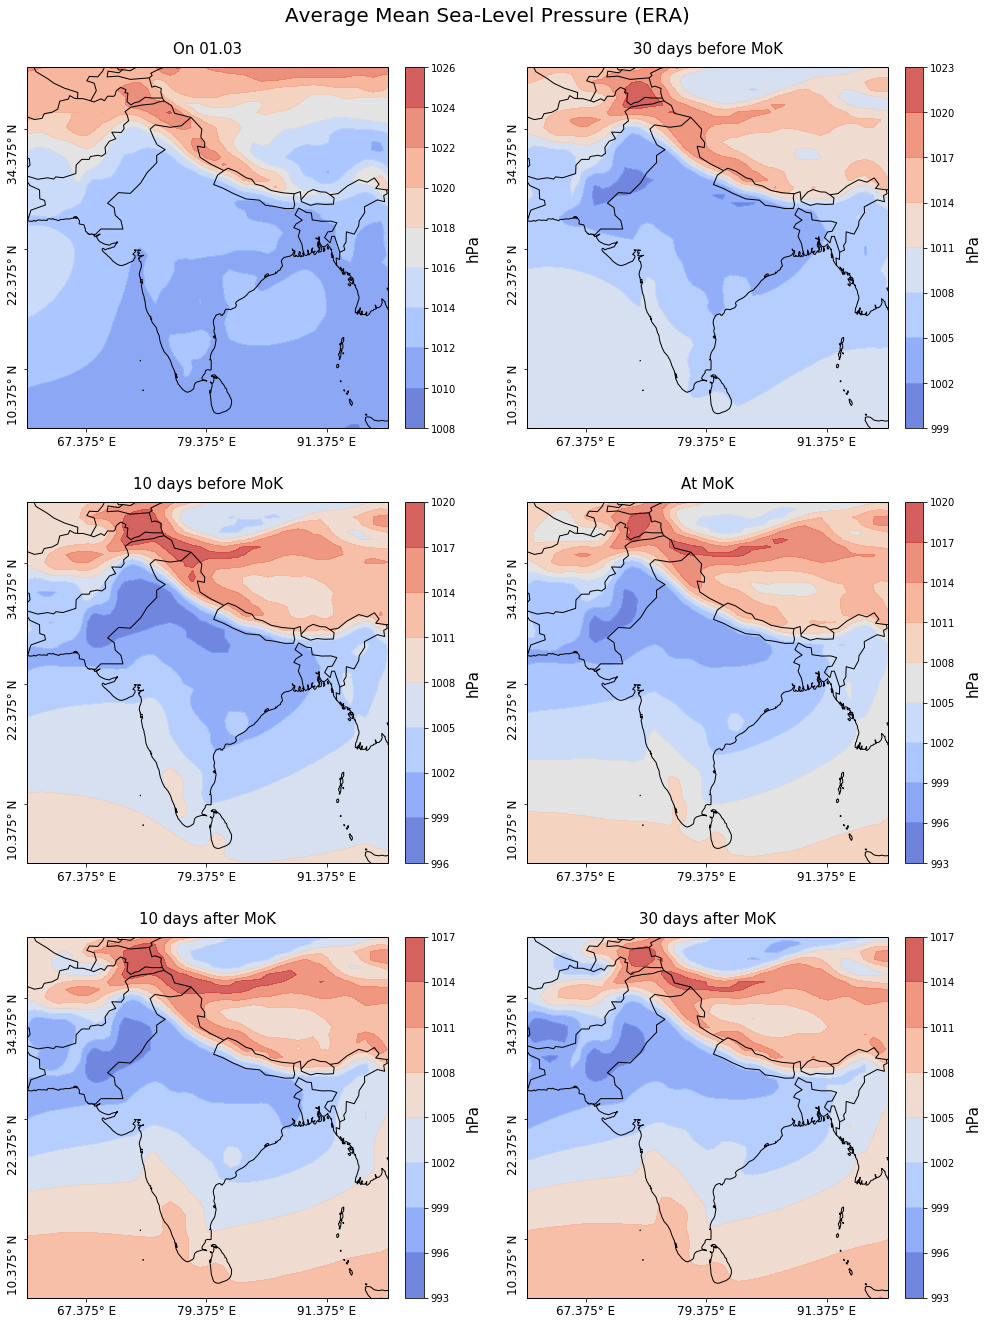
\includegraphics[width=\linewidth]{./99_appendix/img/msl_avg}
  \caption{Average Mean Sea-Level Pressure (ERA-Interim, 1979-2017)}
  \label{apx:era_msl}
\end{figure}

\begin{figure}[h]
  \centering
  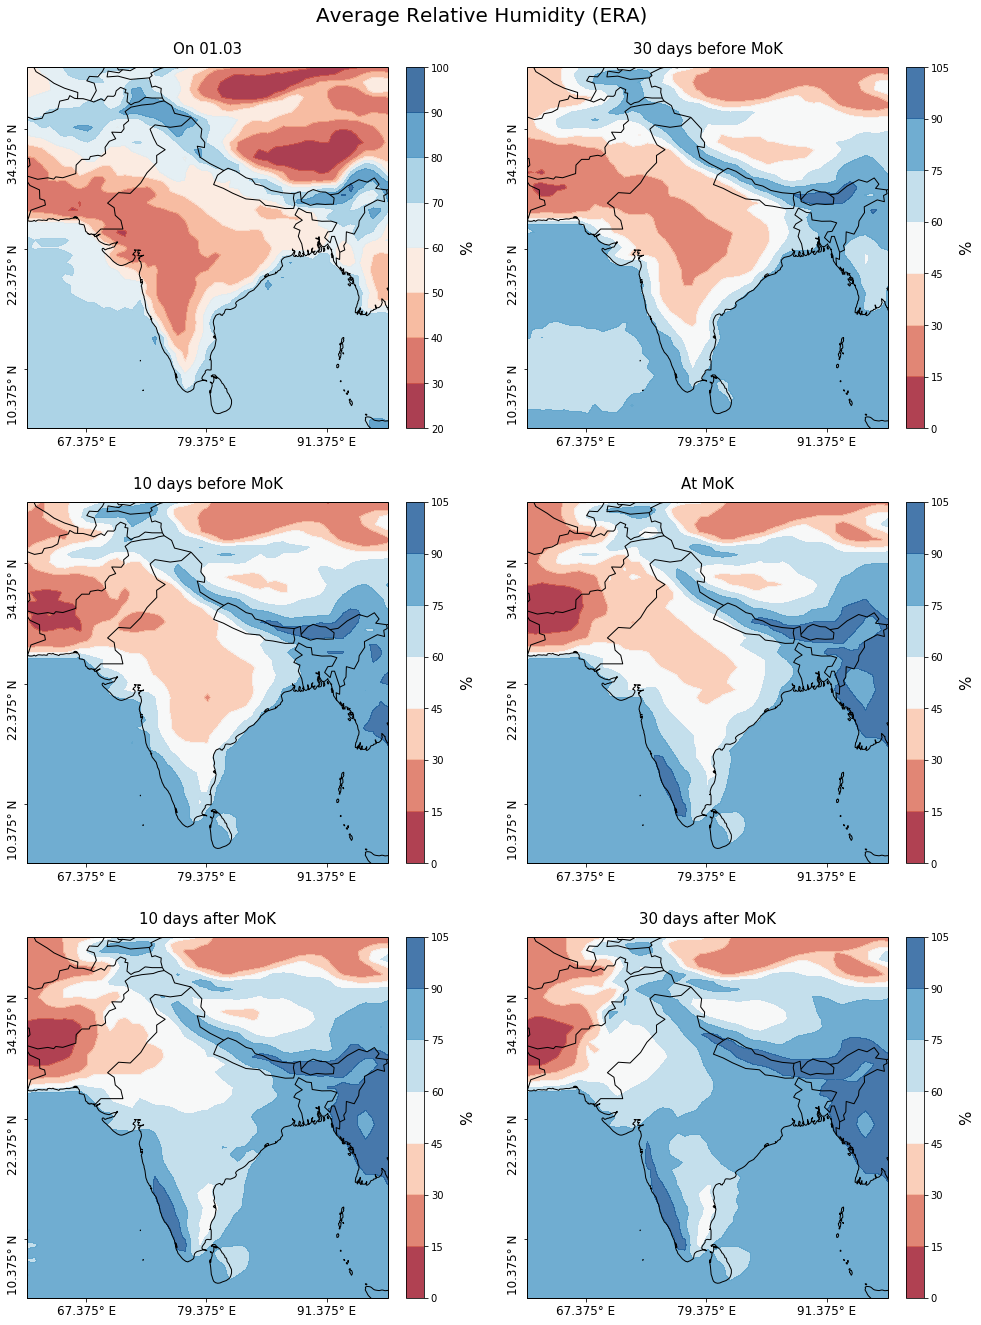
\includegraphics[width=\linewidth]{./99_appendix/img/r_avg}
  \caption{Average Relative Humidity at 1000hPa (ERA-Interim, 1979-2017)}
  \label{apx:era_r}
\end{figure}

\begin{figure}[h]
  \centering
  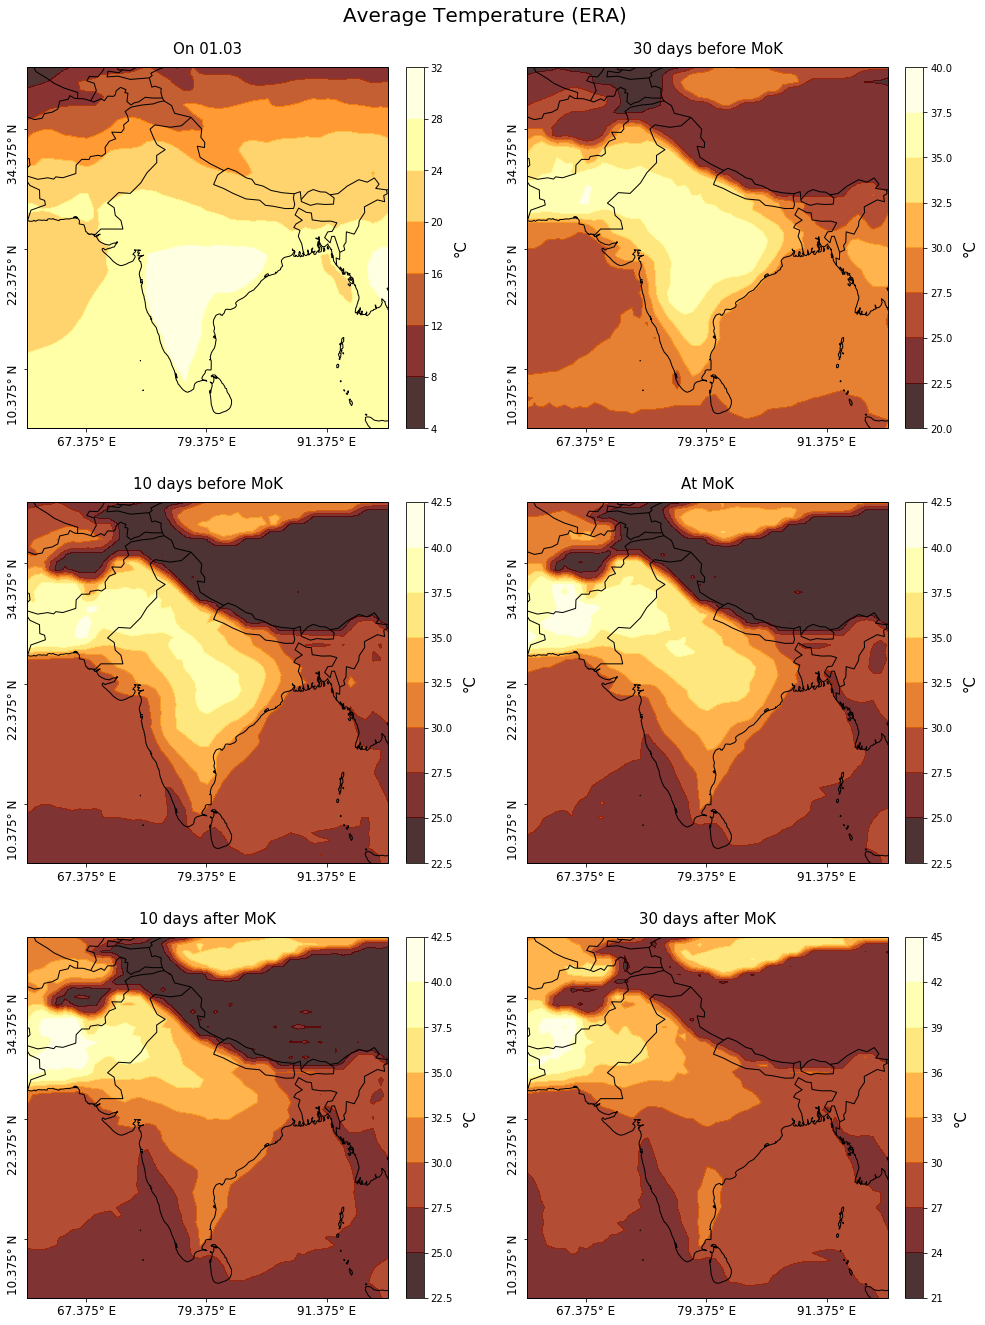
\includegraphics[width=\linewidth]{./99_appendix/img/t_avg}
  \caption{Average Temperature at 1000hPa (ERA-Interim, 1979-2017)}
  \label{apx:era_t}
\end{figure}

\begin{figure}[h]
  \centering
  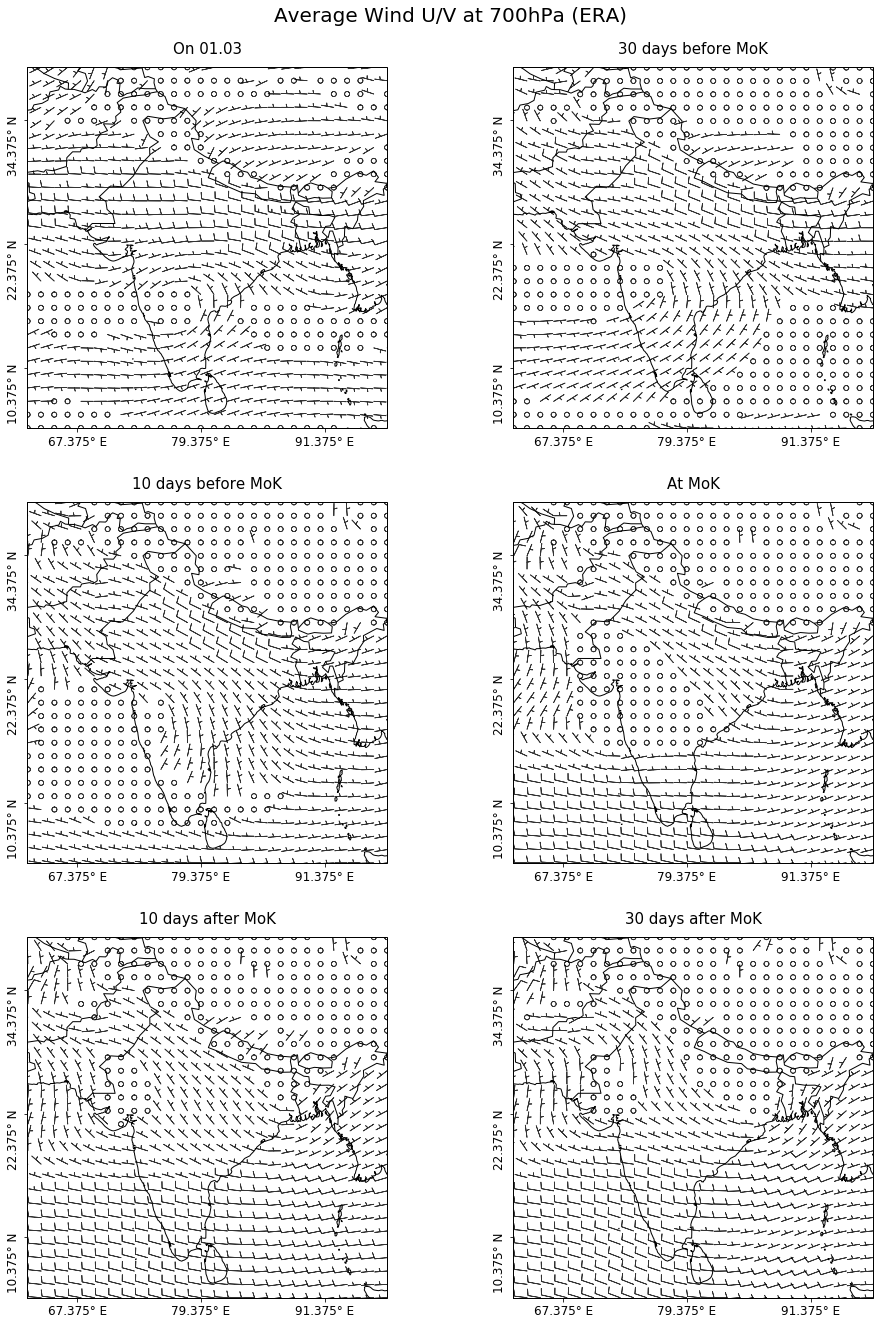
\includegraphics[width=\linewidth]{./99_appendix/img/wind_avg}
  \caption{Average Wind (U/V) at 700hPa (ERA-Interim, 1979-2017)}
  \label{apx:era_wind}
\end{figure}

\begin{figure}[h]
  \centering
  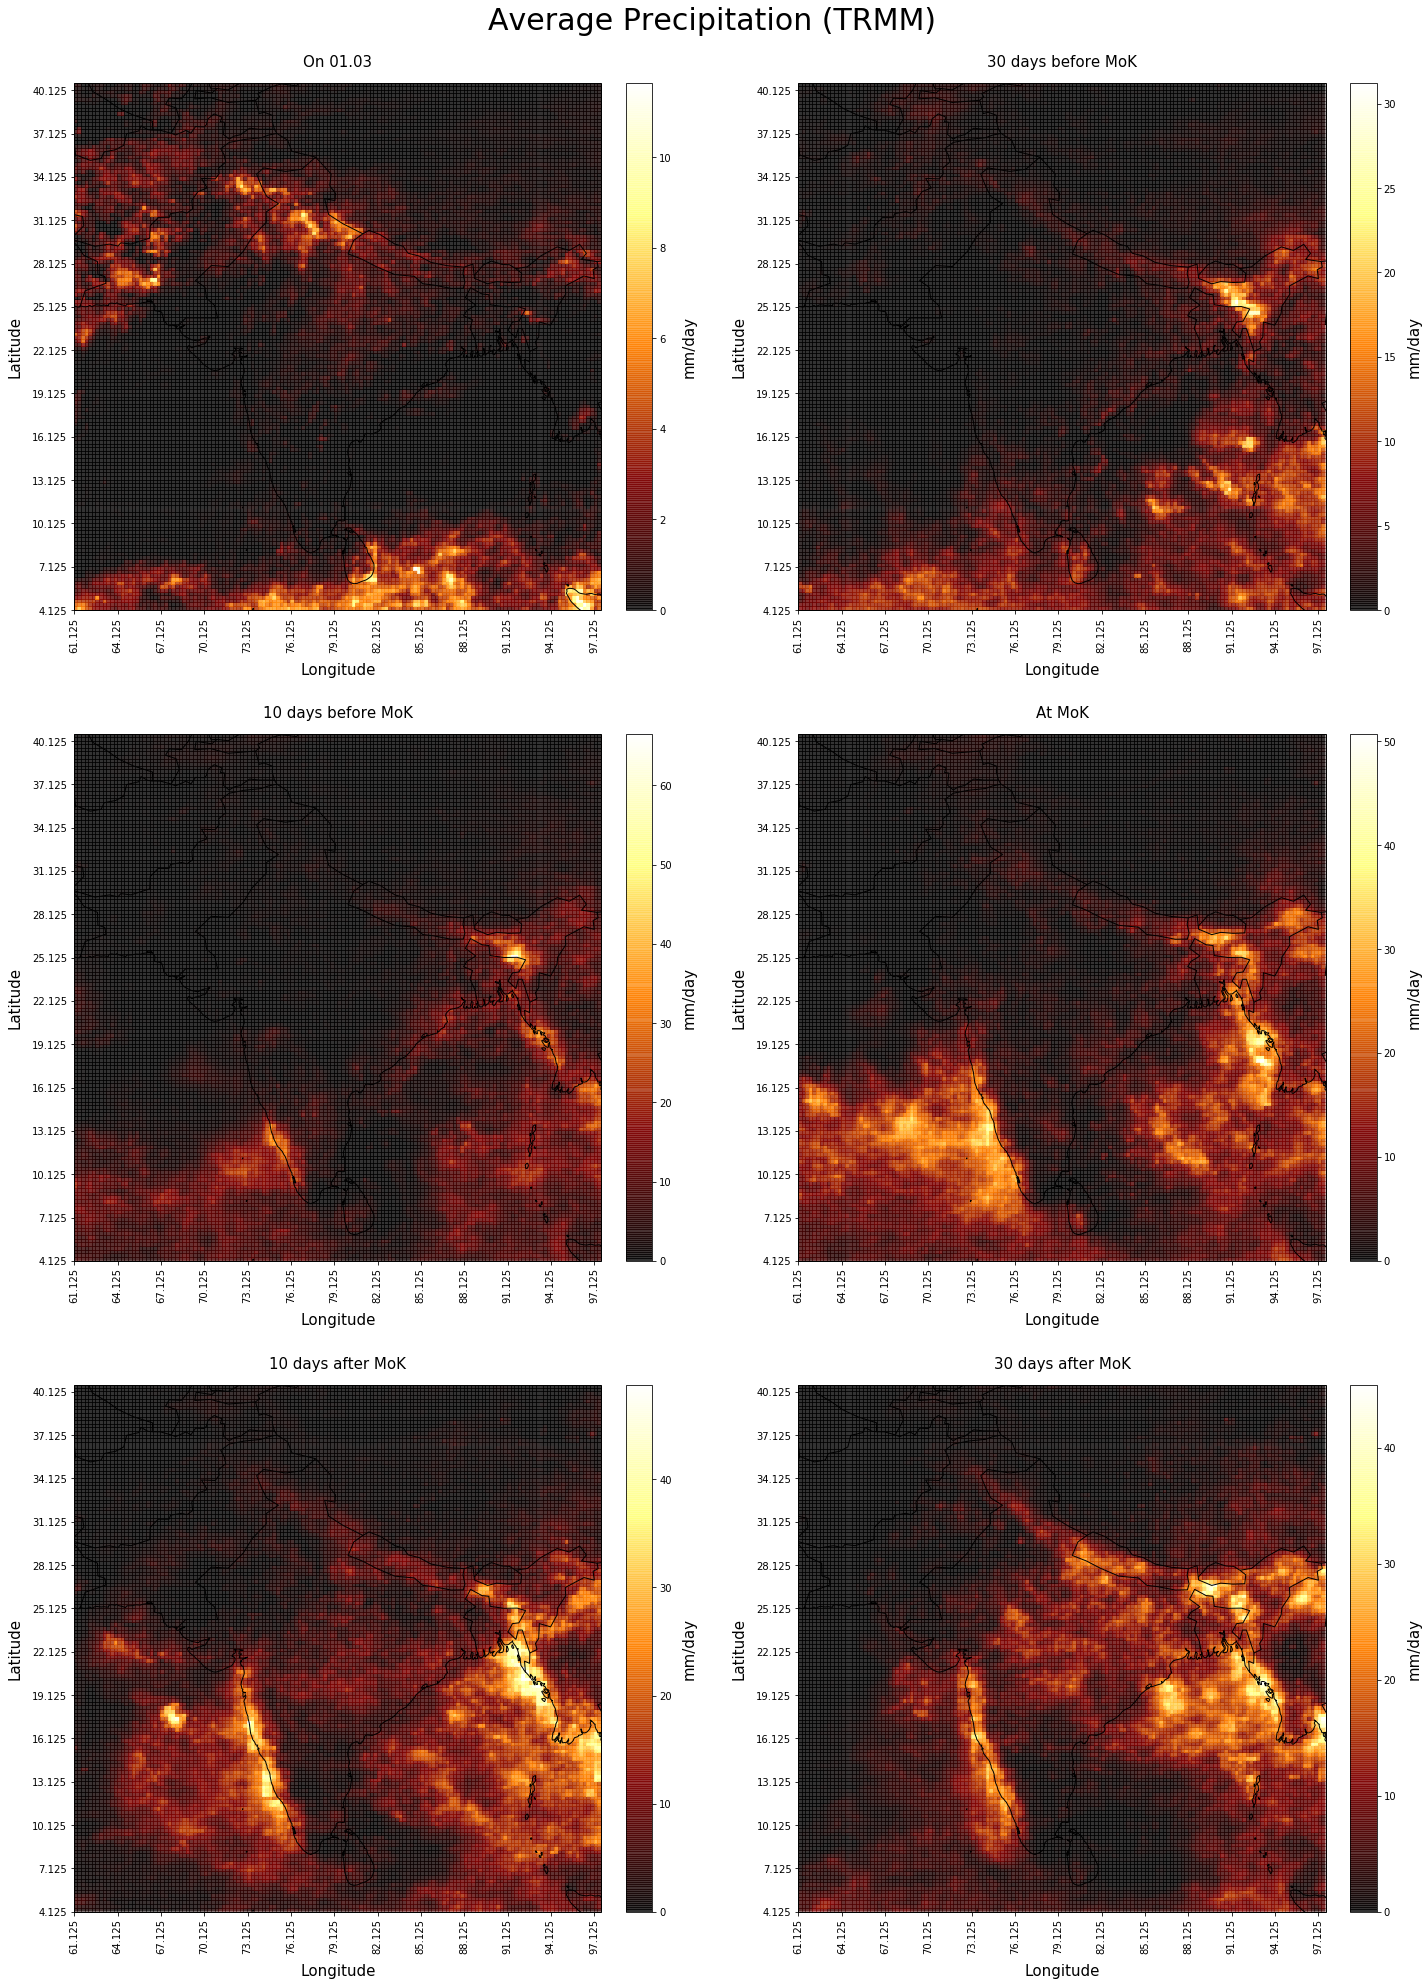
\includegraphics[width=\linewidth]{./99_appendix/img/prec_avg}
  \caption{Average Precipitation (TRMM, 1998-2017)}
  \label{apx:trmm_prec}
\end{figure}

\clearpage
\section{Event Synchronization}
\label{apx:event_sync}

[TODO: labels for rows (degree, betweenness, PageRank)]

\begin{figure}[h]
  \centering
  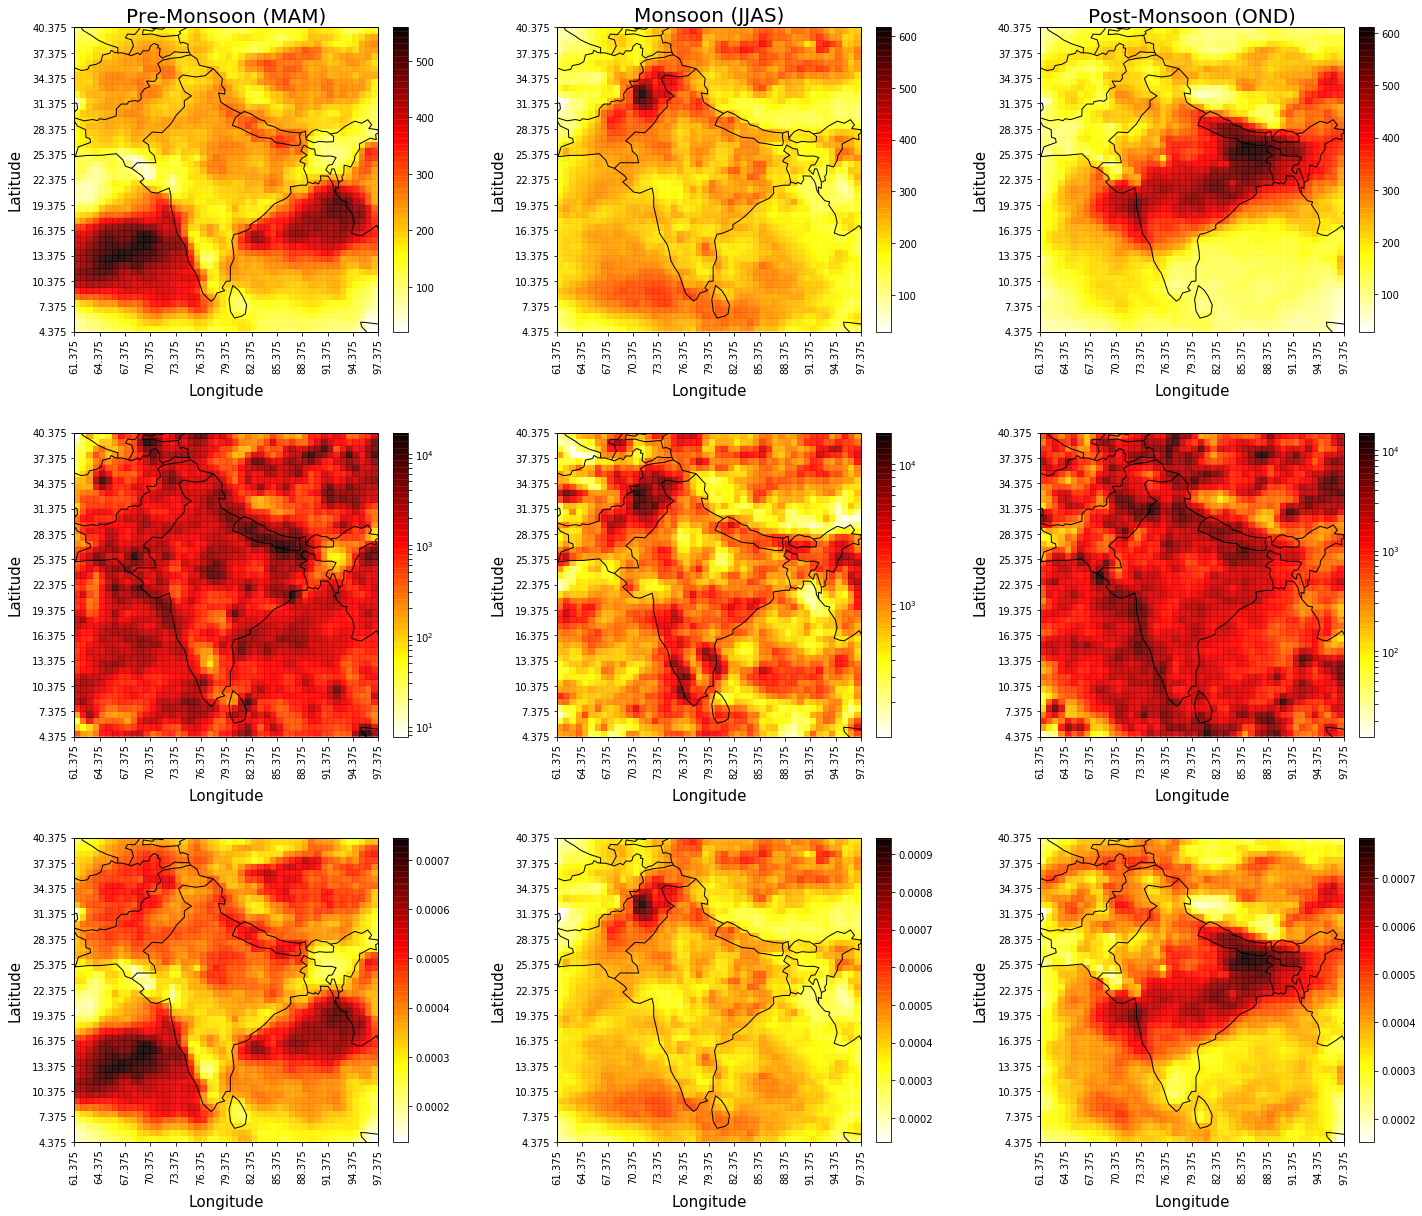
\includegraphics[width=\linewidth]{./99_appendix/img/event_sync_0-75_0-9.png}
  \caption{Event synchronization for unweighted climate networks}
  \label{apx:trmm_prec}
\end{figure}

\begin{figure}[h]
  \centering
  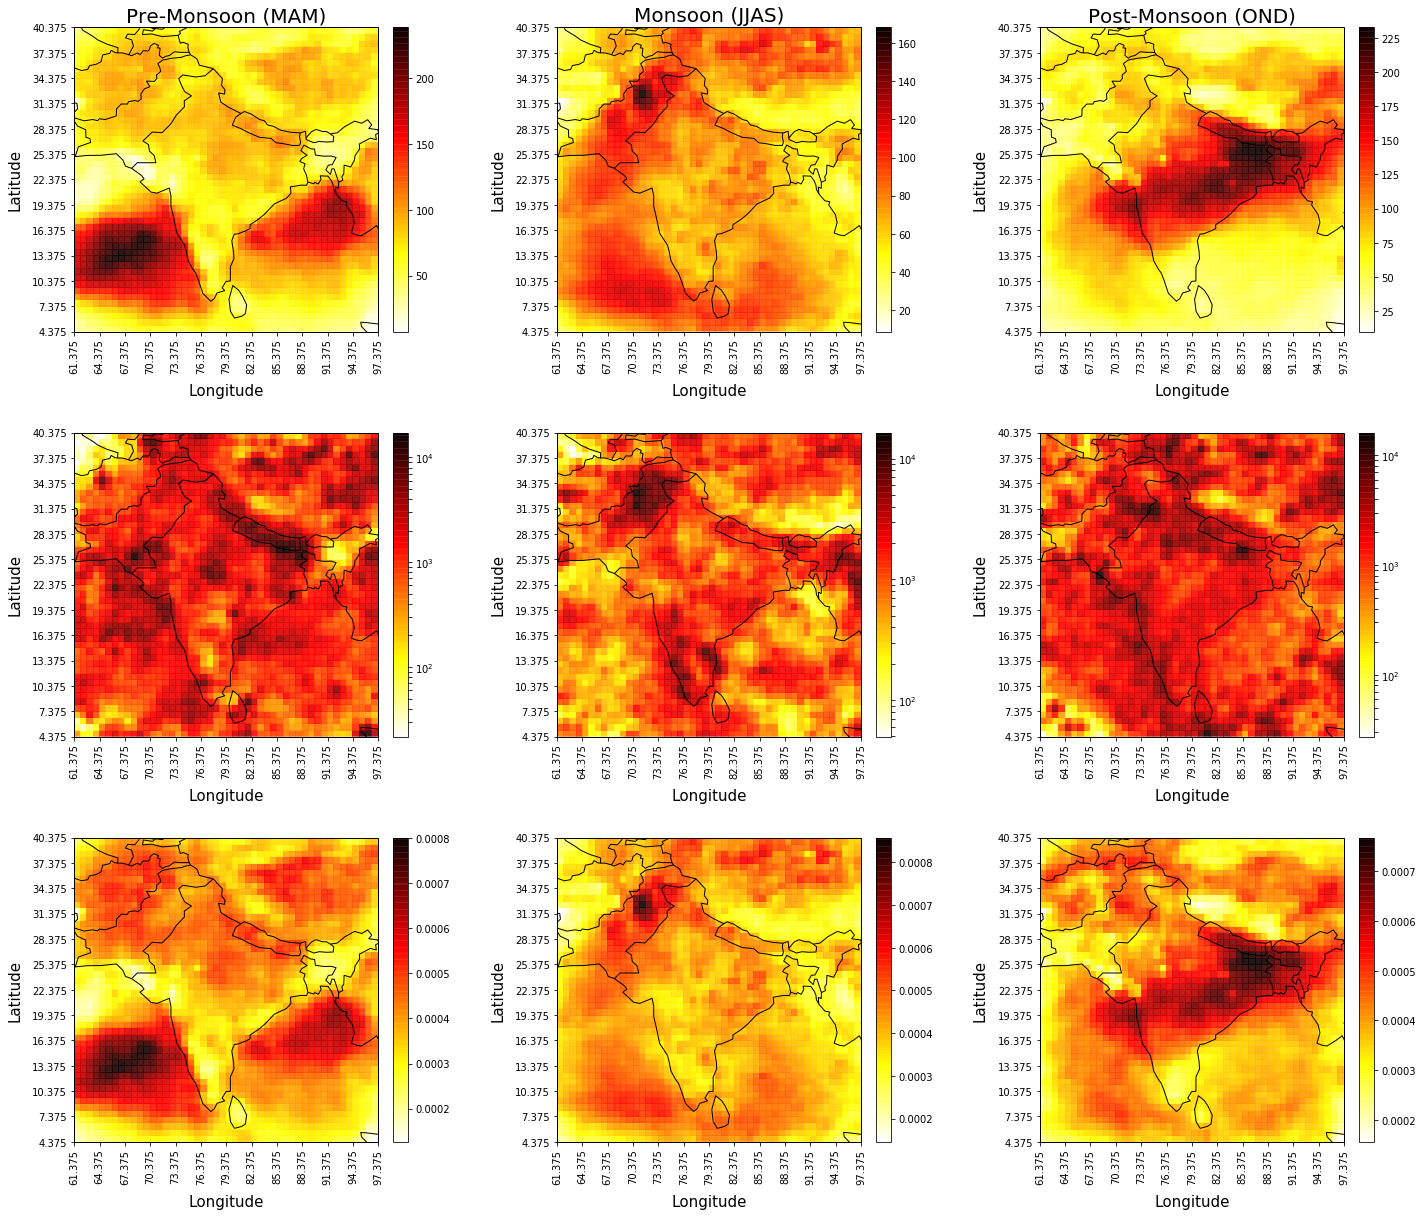
\includegraphics[width=\linewidth]{./99_appendix/img/event_sync_0-75_0-9_weighted.png}
  \caption{Event synchronization for weighted climate networks}
  \label{apx:trmm_prec}
\end{figure}


% *************** Back matter ***************
\backmatter

\normalfont
\clearpage
\listoffigures

\clearpage
\listoftables

\clearpage
\renewcommand\listoflistingscaption{List of source codes}
\listoflistings

\end{document}
